\documentclass[12pt]{article}       % 設定文件類型為 article,字體大小為 12pt
\usepackage[T1]{fontenc}            % 設定 T1 字型編碼,確保特殊字元的正確顯示
\usepackage{lmodern}                % 強制使用 Latin Modern 字型,提高可讀性和相容性
\usepackage{fontspec}               % 允許使用 OpenType 和 TrueType 字型
\usepackage{graphicx}               % 支援插入圖片
\usepackage{amsmath}                % 提供數學環境和公式支持
\usepackage{csquotes}               % 提供引用格式支援
\usepackage{comment}                % 提供多行註解
\usepackage{ragged2e}
\usepackage{float}
\usepackage{diagbox}  % 加入這行來載入 diagbox 套件
\usepackage{booktabs} % 專業表格格式
\usepackage{siunitx}  % 數值對齊
\usepackage{pgfgantt}


%biber Practice_of_Mechanical_Engineering

%=================================================={{{參考文獻設定}}}==================================================

\usepackage[style=ieee, maxnames=99]{biblatex}          % 設定參考文獻格式為 IEEE,最多顯示 99 個作者
\addbibresource{Practice_of_Mechanical_Engineering.bib}                       % 添加參考文獻檔案 references.bib
\renewcommand{\bibfont}{\fontspec{Times New Roman}}     % 設定參考文獻字體為 Times New Roman
\renewcommand{\UrlFont}{\fontspec{Times New Roman}}     % 設定 URL 連結字體為 Times New Roman
\DeclareFieldFormat{url}{\url{#1}}                      % 格式化 URL                          % 引用你的 .bib 文件

%=================================================={{{目錄設定}}}==================================================

\usepackage{tocloft} % 自訂目錄格式

% 設定目錄的點線填充樣式
\renewcommand{\cftsecleader}{\cftdotfill{\cftdotsep}}           % 章節(section)
\renewcommand{\cftsubsecleader}{\cftdotfill{\cftdotsep}}        % 小節(subsection)
\renewcommand{\cftsubsubsecleader}{\cftdotfill{\cftdotsep}}     % 子小節(subsubsection)

% 設定圖目錄與表目錄的點線
\renewcommand{\cftdotsep}{1}  % 設定點的間距,使其在所有目錄(含圖、表)中都有效

% 設定目錄標題格式,使目錄、圖目錄、表目錄標題一致
\renewcommand{\contentsname}{\centering \LARGE \textbf{目錄}}    % 目錄標題置中,加粗
\renewcommand{\listfigurename}{\centering \LARGE \textbf{圖目錄}} % 圖目錄標題置中,加粗
\renewcommand{\listtablename}{\centering \LARGE \textbf{表目錄}} % 表目錄標題置中,加粗


%=================================================={{{字體設定}}}==================================================

% 設定英文字體
\newfontface\englishfont{Times New Roman}               % 自訂英文字體命令 \englishfont,使用 Times New Roman

\setmainfont[
    ItalicFont={Times New Roman Italic},                % 設定斜體
    BoldFont={Times New Roman Bold},                    % 設定粗體
    BoldItalicFont={Times New Roman Bold Italic}        % 設定粗斜體
]{Times New Roman}                                      % 設定主要英文字體為 Times New Roman

% 設定中文字體

\usepackage{xeCJK}                                      % 使用 xeCJK 宏包以支援中文
\renewcommand{\figurename}{圖}                           % 設定圖表名稱
\renewcommand{\tablename}{表}                            % 修改表格標題為「表」
\setCJKmainfont[BoldFont={標楷體-繁}, ItalicFont={標楷體-繁}] {標楷體-繁}

%=================================================={{{版面設定}}}==================================================

% 設定頁面邊界,適用 A4 紙張
\usepackage[top=2.54cm, bottom=2.54cm, left=3.18cm, right=3.18cm, a4paper]{geometry}

% 設定行距與段落格式
\usepackage{setspace}
\onehalfspacing % 設定 1.5 倍行距
\setlength{\parskip}{6pt} % 設定段落間距 6pt
\setlength{\parindent}{2em} % 設定段落首行縮排 2 個字元

%=============================================================================================================================
%=============================================================================================================================
%=============================================================================================================================

\begin{document}
%=================================================={{{封面}}}==================================================
\begin{titlepage}
    \centering
    \vspace*{1cm} % 增加上方間距

    {\LARGE \textbf{元智大學工程學院機械工程學系}} \\[0.5cm] % 標題較大且加粗
    {\LARGE {Department of Mechanical Engineering}} \\[0.5cm] % 標題較大且加粗
    {\LARGE {College of Engineering}} \\[0.5cm]
    {\LARGE {Yuan Ze University}}

    \vfill % 這一行讓前面的資訊靠上排列

    {\LARGE{孤輪阿罵的飆速輪椅}} \\[0.5cm]% 這行會上下左右完全置中
    {\LARGE{機械工程實務進度報告1}} % 這行會上下左右完全置中

    \vfill % 這一行讓後面的資訊靠下排列

    {\LARGE {1100826 王子晨}}\\[0.5cm]
    {\LARGE {1100854 蘇威全}}\\[0.5cm]
    {\LARGE {1100862 施廷翰}}\\[0.5cm]
    {\LARGE {1100812 魏羽暘}}\\[0.5cm]
    {\LARGE {1100861 盧昀序}}\\[2.5cm]
    {\LARGE {指導教授:江右君、翁芳柏、余念一、吳昌暉}}\\[0.5cm]

\end{titlepage}
\newpage
%=================================================={{{封面}}}==================================================

\pagenumbering{roman}  
\setcounter{page}{1}  % 從 I 開始

%=================================================={{{中文摘要}}}==================================================

\section*{\centering 摘要}  % 只讓標題置中
\addcontentsline{toc}{section}{摘要}  % 手動加入摘要到目錄

%==============================摘要內容==============================

\hspace{2em}

\vspace{1.5em}
\noindent 關鍵字:
%==============================摘要內容==============================
\newpage  % 插入換頁命令,將目錄和後續內容分開

%=================================================={{{英文摘要}}}==================================================
\section*{\centering Abstract}  % 只讓標題置中
\addcontentsline{toc}{section}{Abstract}  % 手動加入摘要到目錄
%==============================摘要內容==============================
\hspace{2em}

\vspace{1.5em}
\noindent Keyword: 
%==============================摘要內容==============================
\newpage  % 插入換頁命令,將目錄和後續內容分開

%=================================================={{{目錄}}}==================================================

\begin{center}
    \tableofcontents    % 生成目錄
%========================={{{可有可無}}}=========================
    \newpage 

    \addtocontents{toc}{\protect\setcounter{tocdepth}{0}} % 暫時關閉目錄深度,讓圖目錄不顯示在目錄中
    \listoffigures      % 生成圖目錄
    \addtocontents{toc}{\protect\setcounter{tocdepth}{2}} % 恢復目錄深度(如果你的章節結構需要更深層級,請調整數值)
    \newpage  
    \listoftables       % 生成表目錄

%========================={{{可有可無}}}=========================
\end{center} 
%=================================================={{{內容開始}}}==================================================
\newpage  % 插入換頁命令,將目錄和後續內容分開
\pagenumbering{arabic}  % 開始使用阿拉伯數字頁碼
\setcounter{page}{1}  % 設定頁碼從 1 開始

%\englishfont{this is an example of mixed English and Chinese.}

\section{\centering 緒論}

\subsection{問題敘述} 
%==============================內文==============================
\hspace{2em}
\begin{itemize}
    \item 測試開始前車輛需整車放置於起跑區中,感測器可與框線 
    對齊。
    \item 車輛完全自主循跡,以自主風力驅動,不得以遙控或遠端 
    修改程式控制車輛。
    \item 測試時間內可隨時返回起跑區重新測試,取單趟最短完成 
    時間為期末展現分數依據。測試時間為5分鐘。
    \item 測試過程中有下述違規事項者,返回起跑區域重新開始, 
    期間不停錶
    \item 未照循跡行進:
    \begin{enumerate}
        \item 行進過程中,車體有部分離開賽道範圍(以區域框線外緣 
        為準)
        \item 於暫停區和終點區時,車體全部投影面積需靜止於區內 
        至少3秒
        \item 以外力碰觸或影響車體
    \end{enumerate}
\end{itemize}

競賽跑道規格如下圖所示。
\begin{figure}[H]
    \centering
    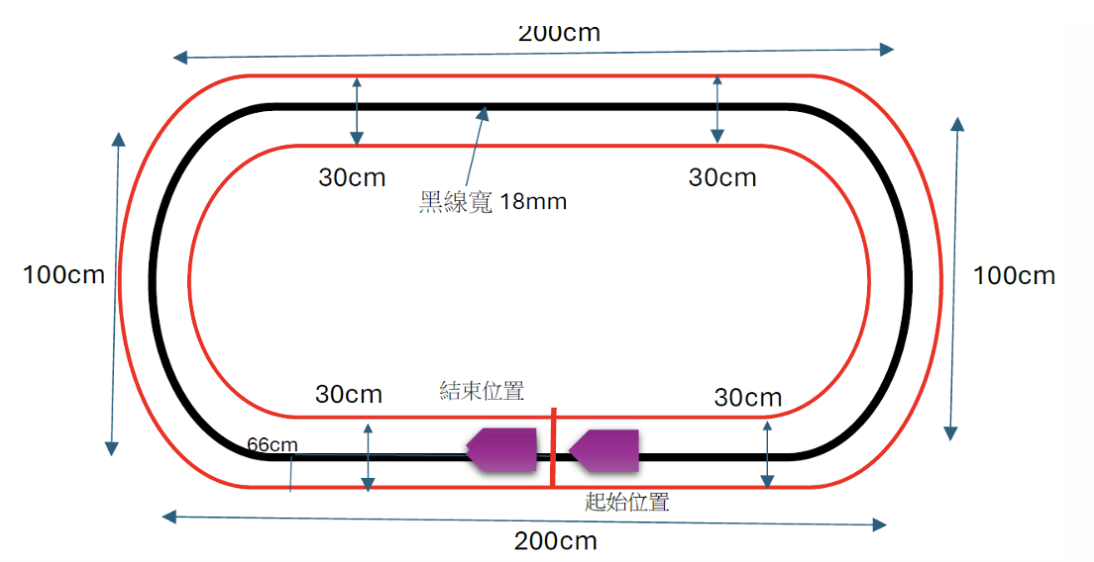
\includegraphics[width=0.7\textwidth]{1.jpg}     %圖片檔案名稱
    \caption{競賽跑道}    %圖片檔案名稱
    \label{fig:1}    %為圖片添加標籤
    %如\ref{fig:example1}所示
\end{figure}
%==============================內文==============================

\subsection{設計規範} 
%==============================內文==============================
\hspace{2em}
\begin{enumerate}
    \item 車體大小不超過A4(21.0 cm $\times$ 29.7 cm)。 
    \item 車輛僅用風力驅動,不得有其他動力來源。 
    至少3秒
    \item 扇葉需自行設計製造,且須帶有保護裝置以防扇葉 
    飛出造成傷害。 
    \item 車體載重設計須外加負載250g,模擬車手重量。 
    \item 最終總成本不得超過3000 元新台幣,且所有元件皆 
    需發票或加工證明,不可外包。 
    \item 機電系統需自行組裝與測試,可購買市售相關零組件。 
\end{enumerate}
%==============================內文==============================

\subsection{任務分工} 
%==============================內文==============================


\begin{itemize}
    \item 1100826 王子晨:演算法設計、期末報告撰寫
    \item 1100854 蘇威全:風扇設計、流力分析
    \item 1100862 施廷翰:車體設計
    \item 1100812 魏羽暘:簡報製作
    \item 1100861 盧昀序:製作阿罵
\end{itemize}

%==============================內文==============================

\section{\centering 設計理念}

\subsection{車體設計} 

\subsubsection{車體結構}
%==============================內文==============================
\hspace{2em}
\begin{figure}[H]
    \centering
    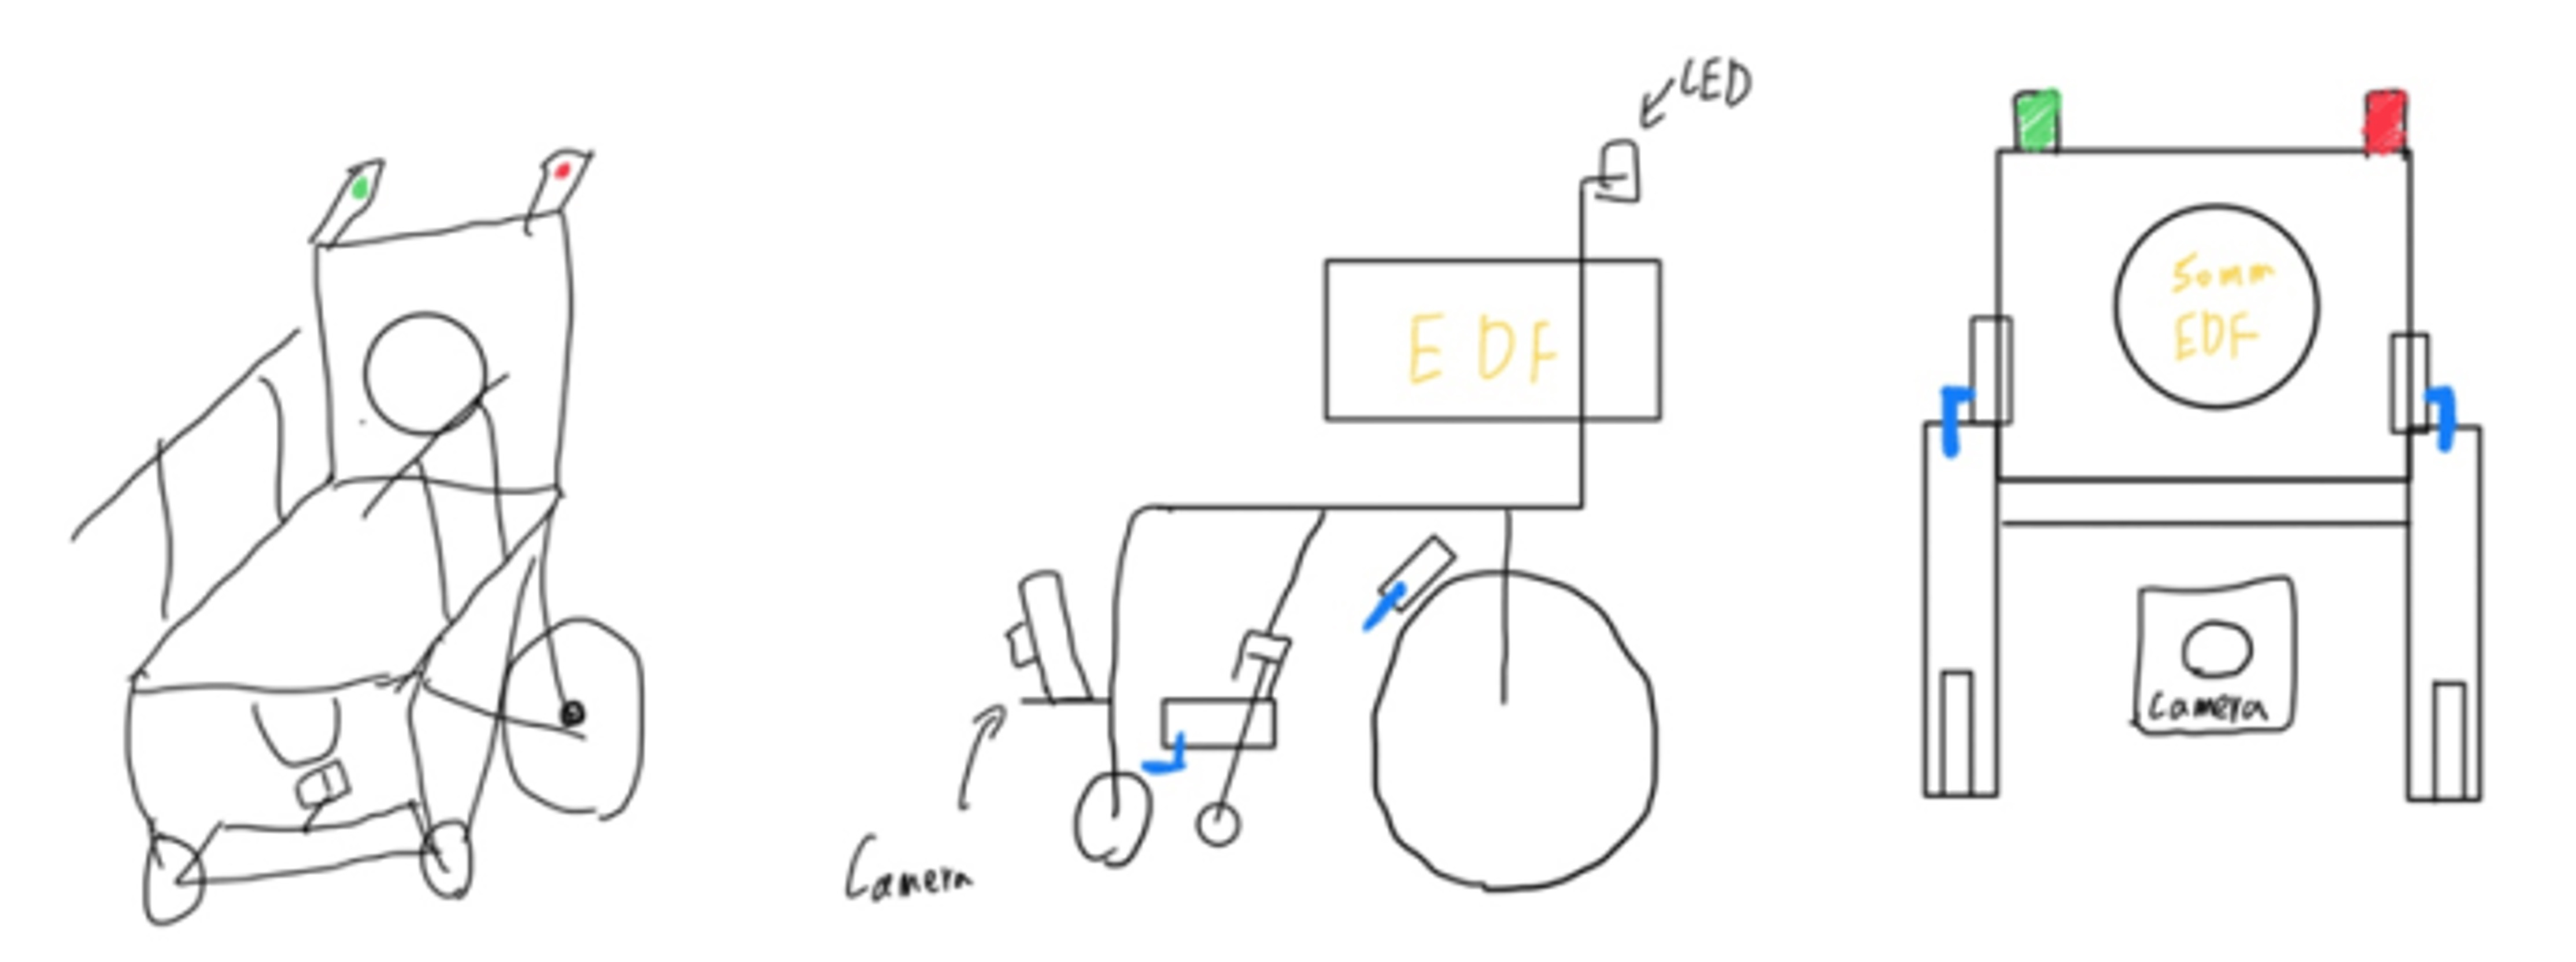
\includegraphics[width=0.7\textwidth]{2.jpg}     %圖片檔案名稱
    \caption{車體結構草圖}    %圖片檔案名稱
    \label{fig:2}    %為圖片添加標籤
    %如\ref{fig:example1}所示
\end{figure}
%==============================內文==============================

\subsubsection{影像辨識系統}
%==============================內文==============================
\hspace{2em}
\begin{figure}[H]
    \centering
    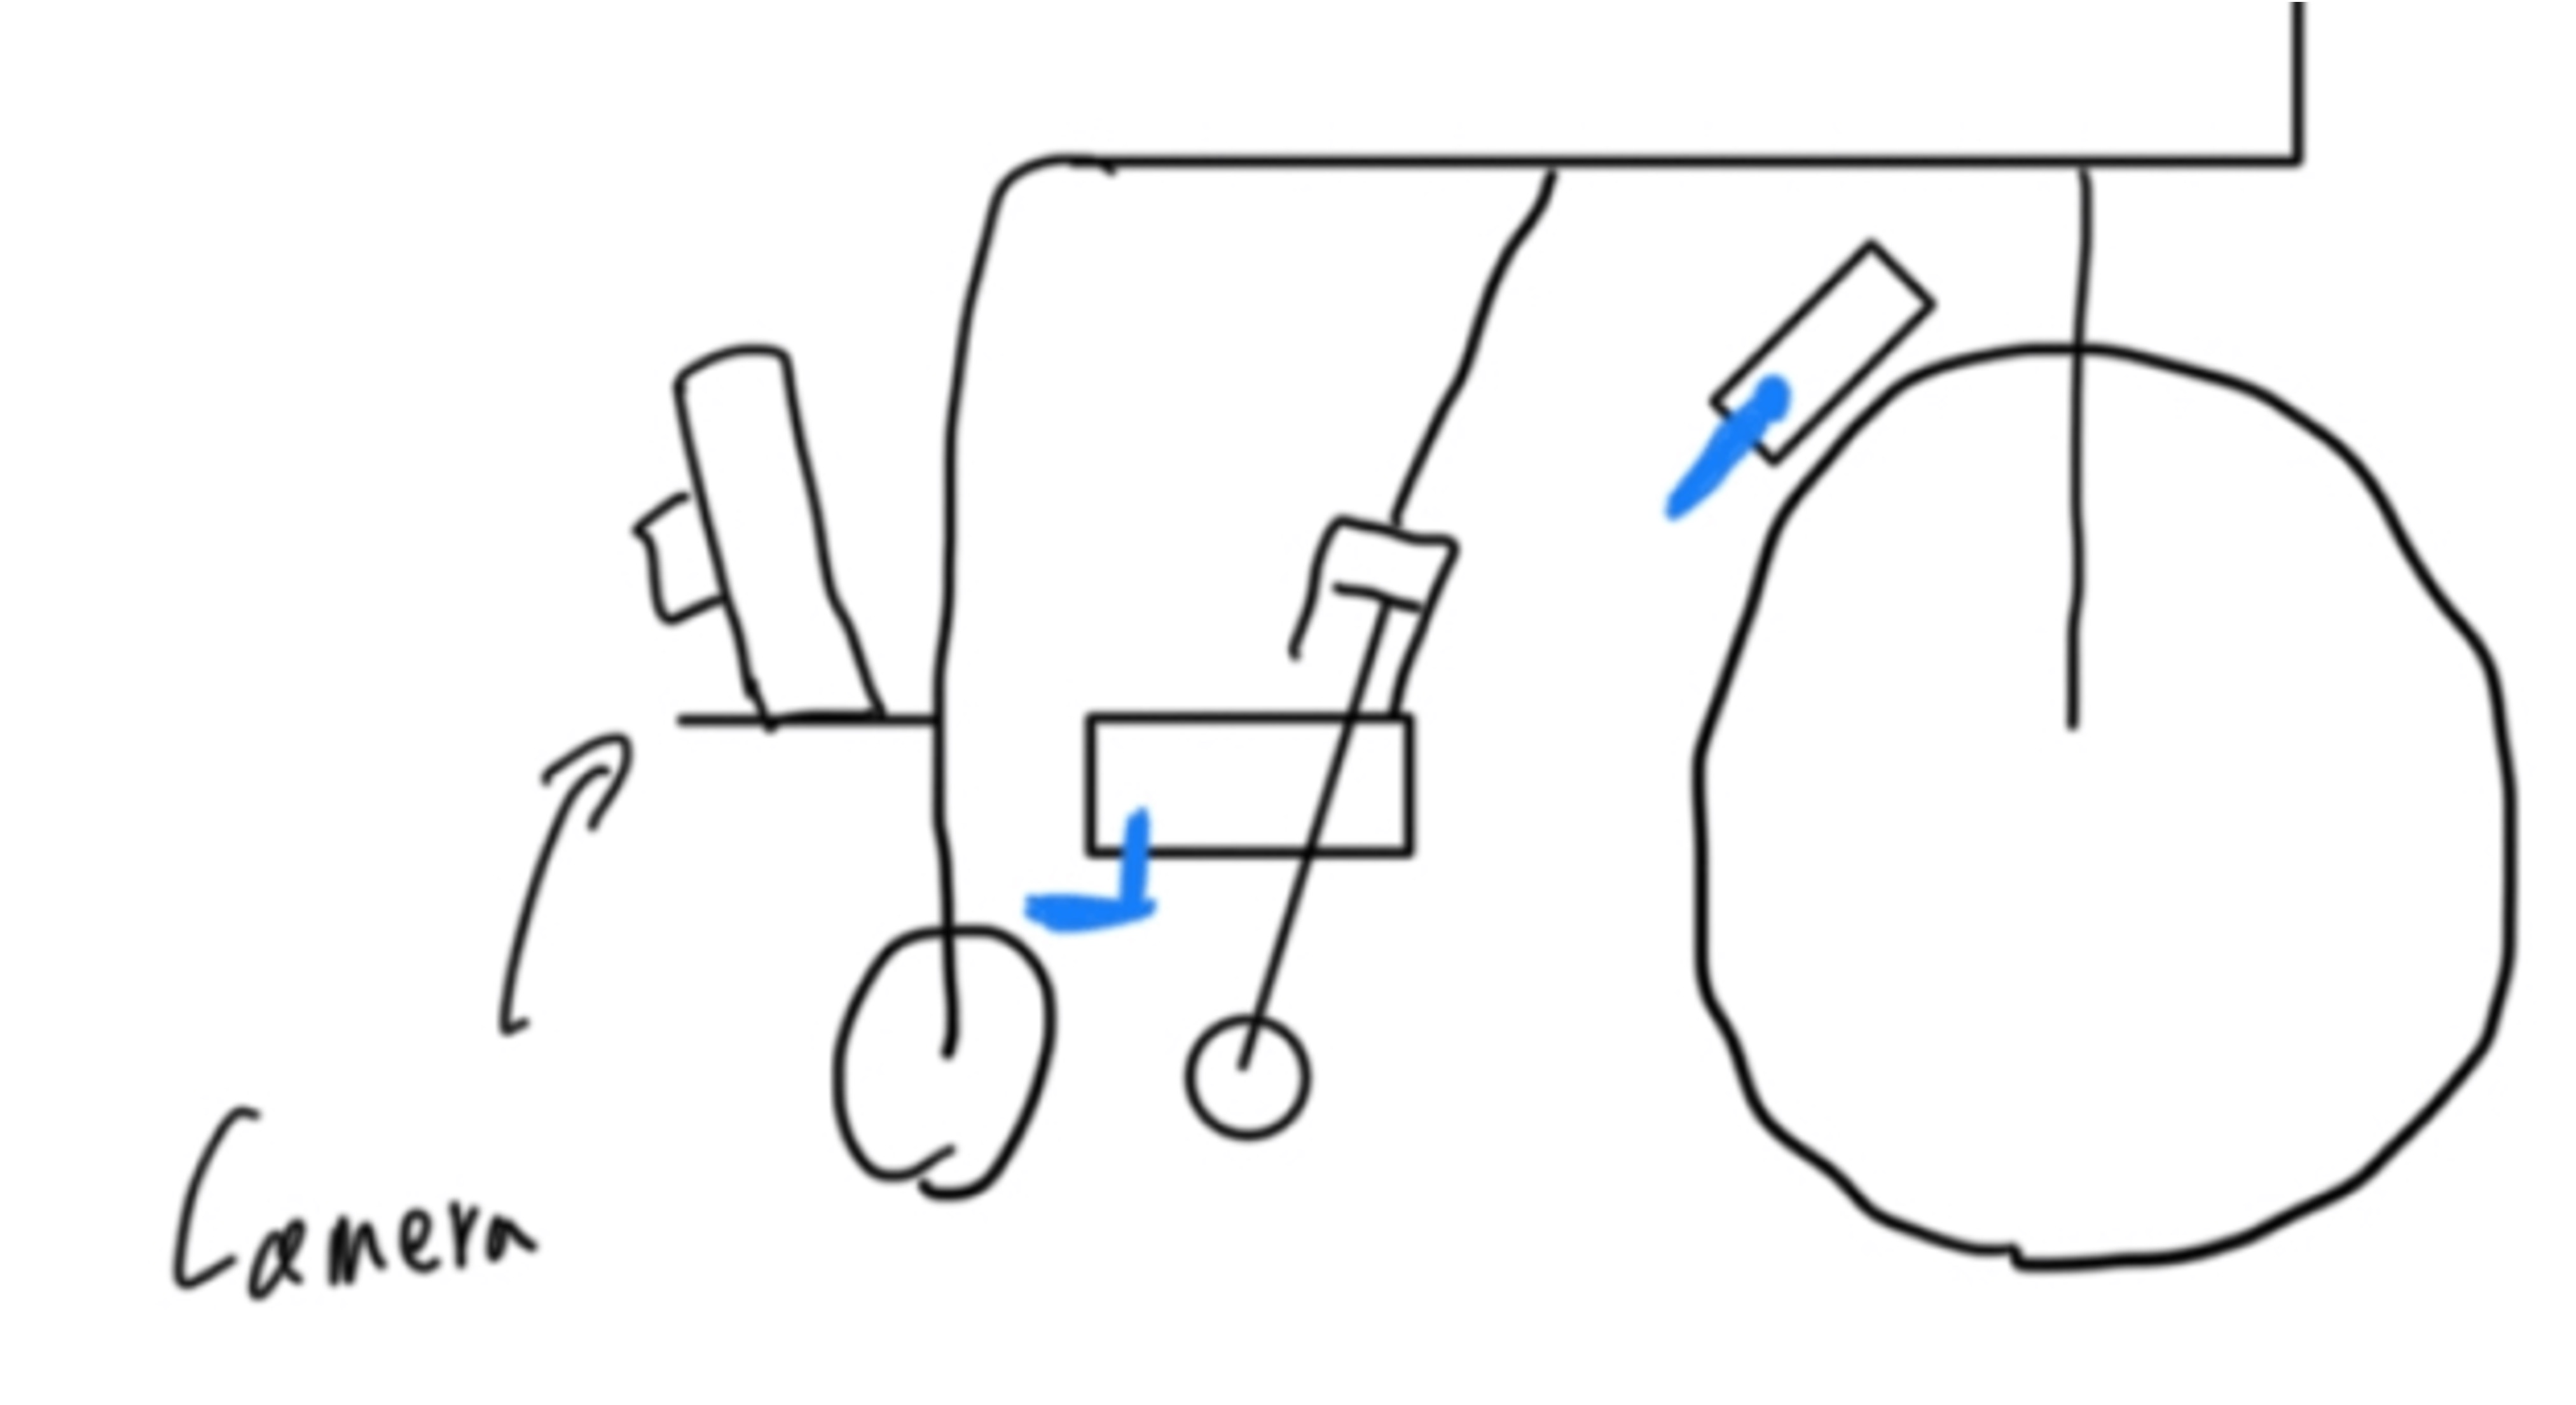
\includegraphics[width=0.7\textwidth]{3.jpg}     %圖片檔案名稱
    \caption{影像辨識系統草圖}    %圖片檔案名稱
    \label{fig:3}    %為圖片添加標籤
    %如\ref{fig:example1}所示
\end{figure}
%==============================內文==============================

\subsubsection{轉向、燈光系統}
%==============================內文==============================
\hspace{2em}
\begin{figure}[H]
    \centering
    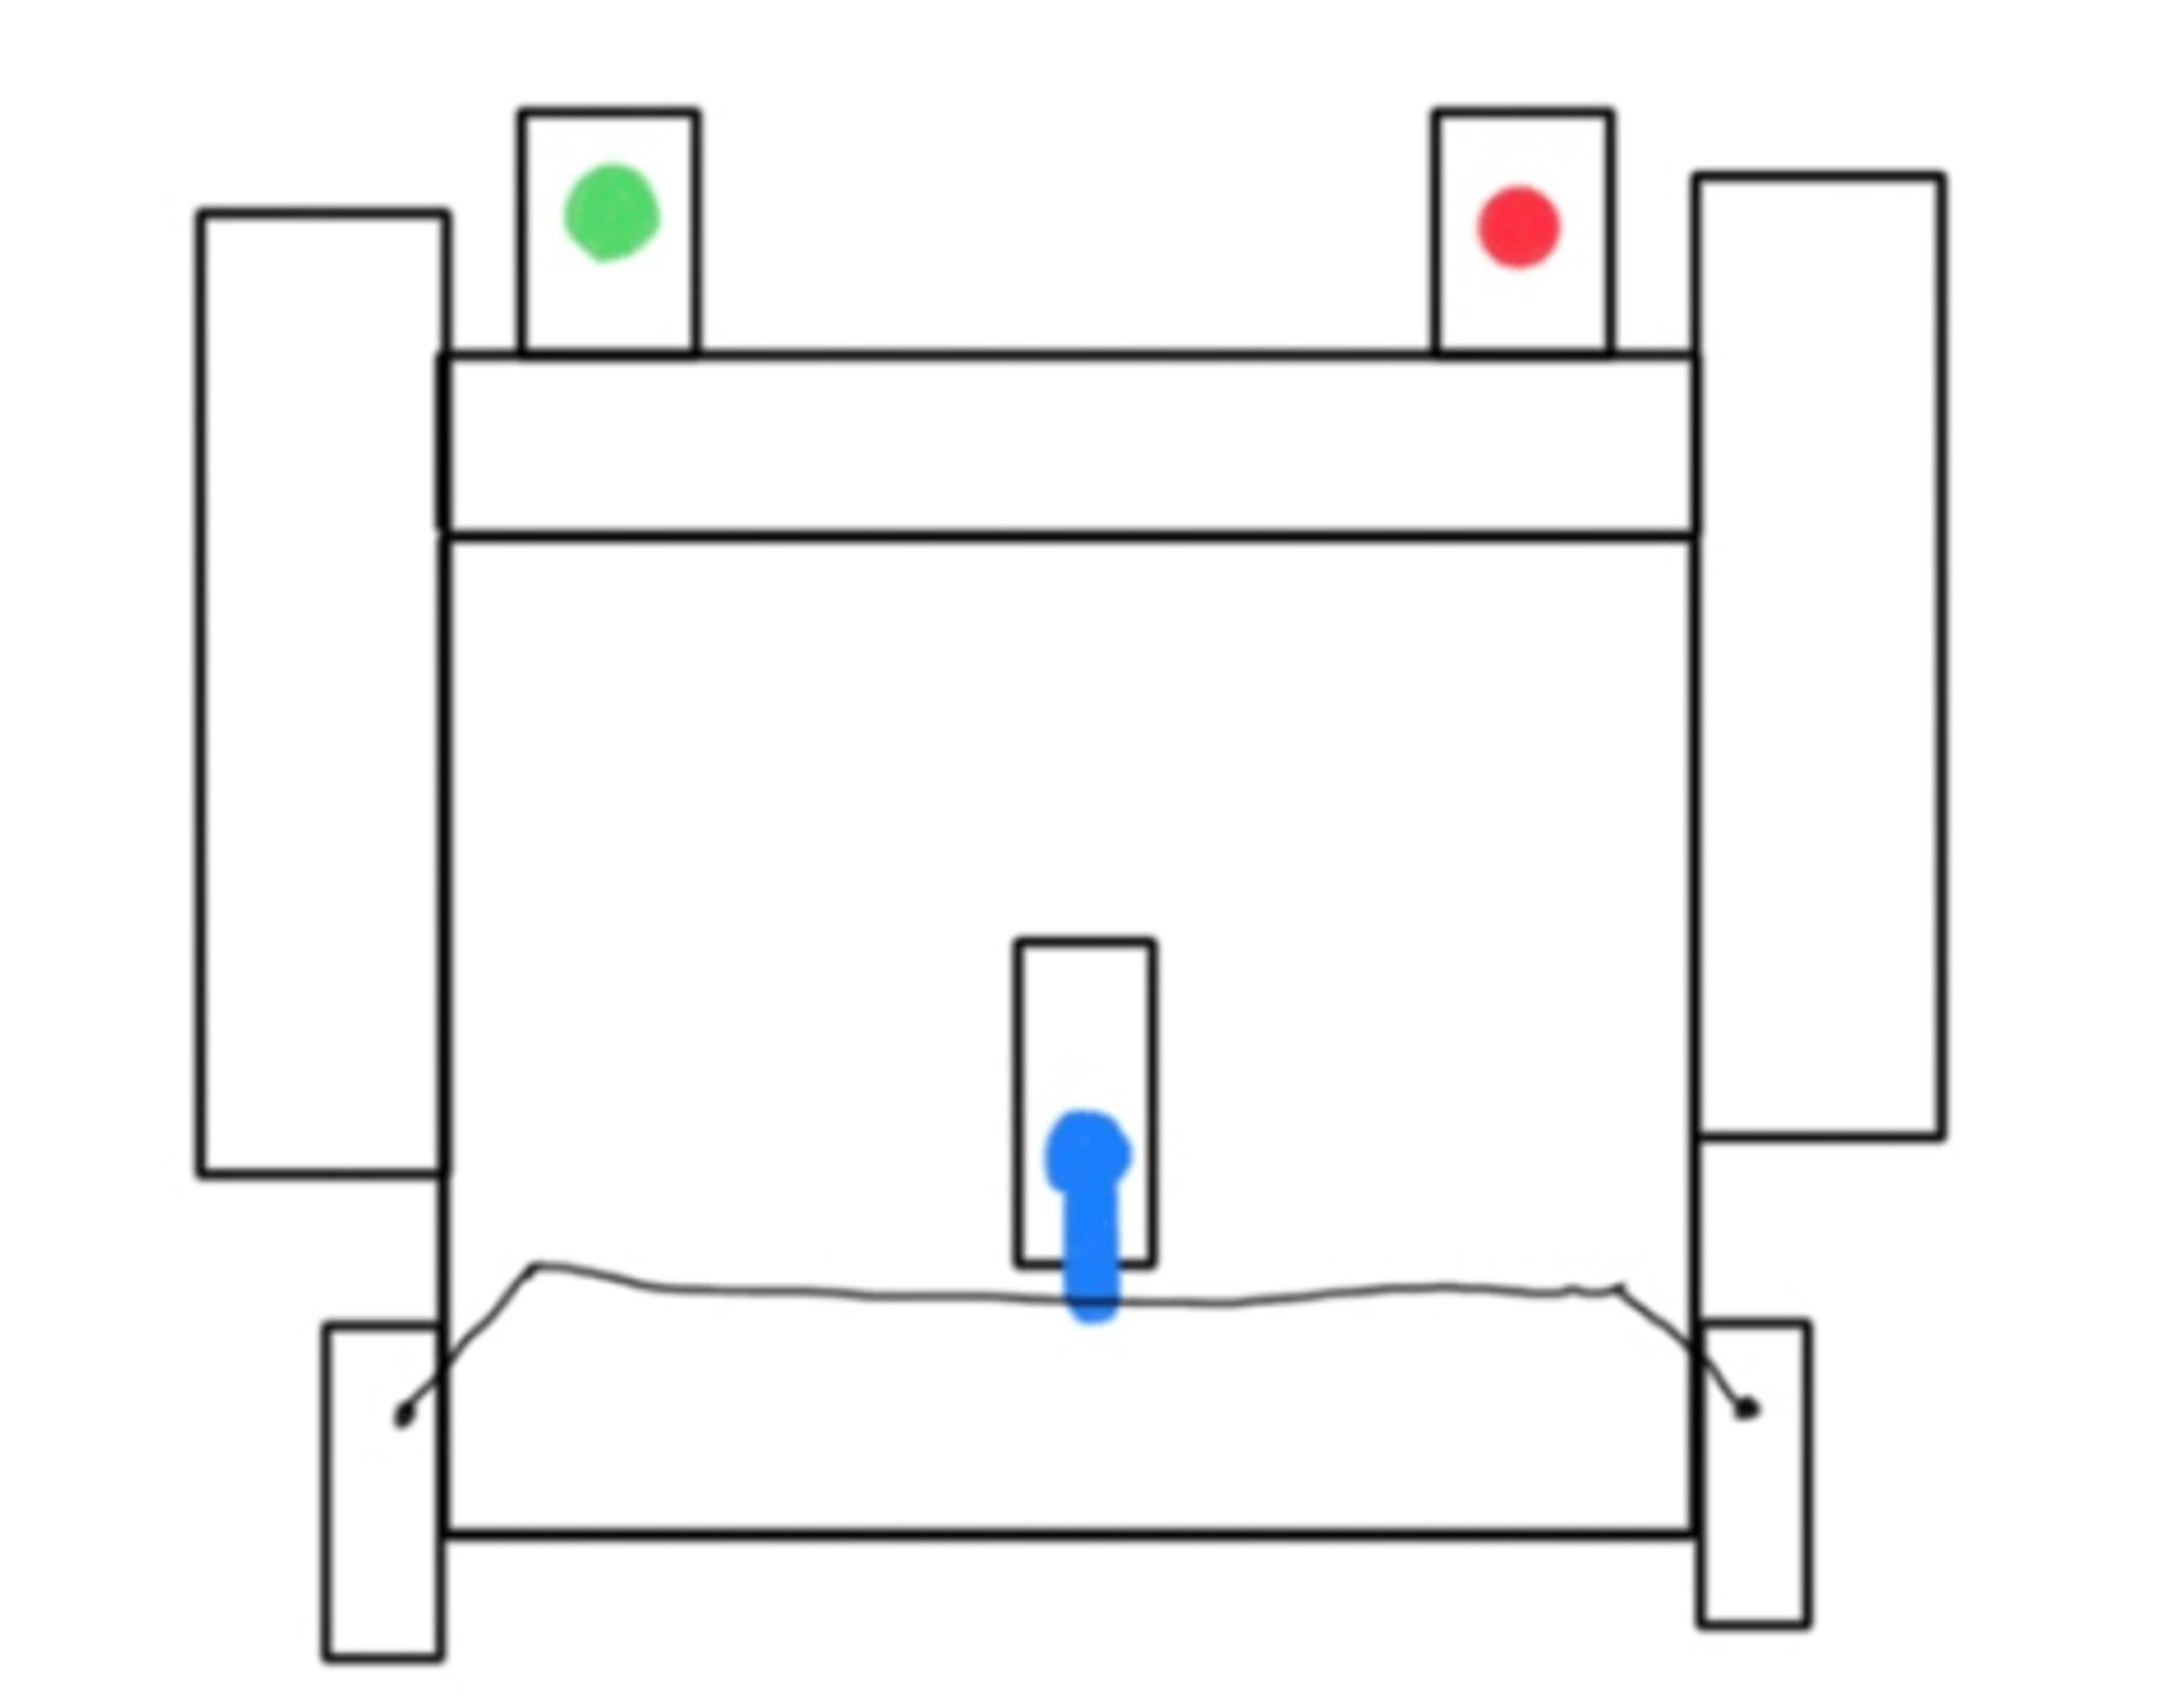
\includegraphics[width=0.7\textwidth]{4.jpg}     %圖片檔案名稱
    \caption{轉向、燈光系統草圖}    %圖片檔案名稱
    \label{fig:4}    %為圖片添加標籤
    %如\ref{fig:example1}所示
\end{figure}
%==============================內文==============================

\subsubsection{自動控制系統}
%==============================內文==============================
\hspace{2em}
\begin{figure}[H]
    \centering
    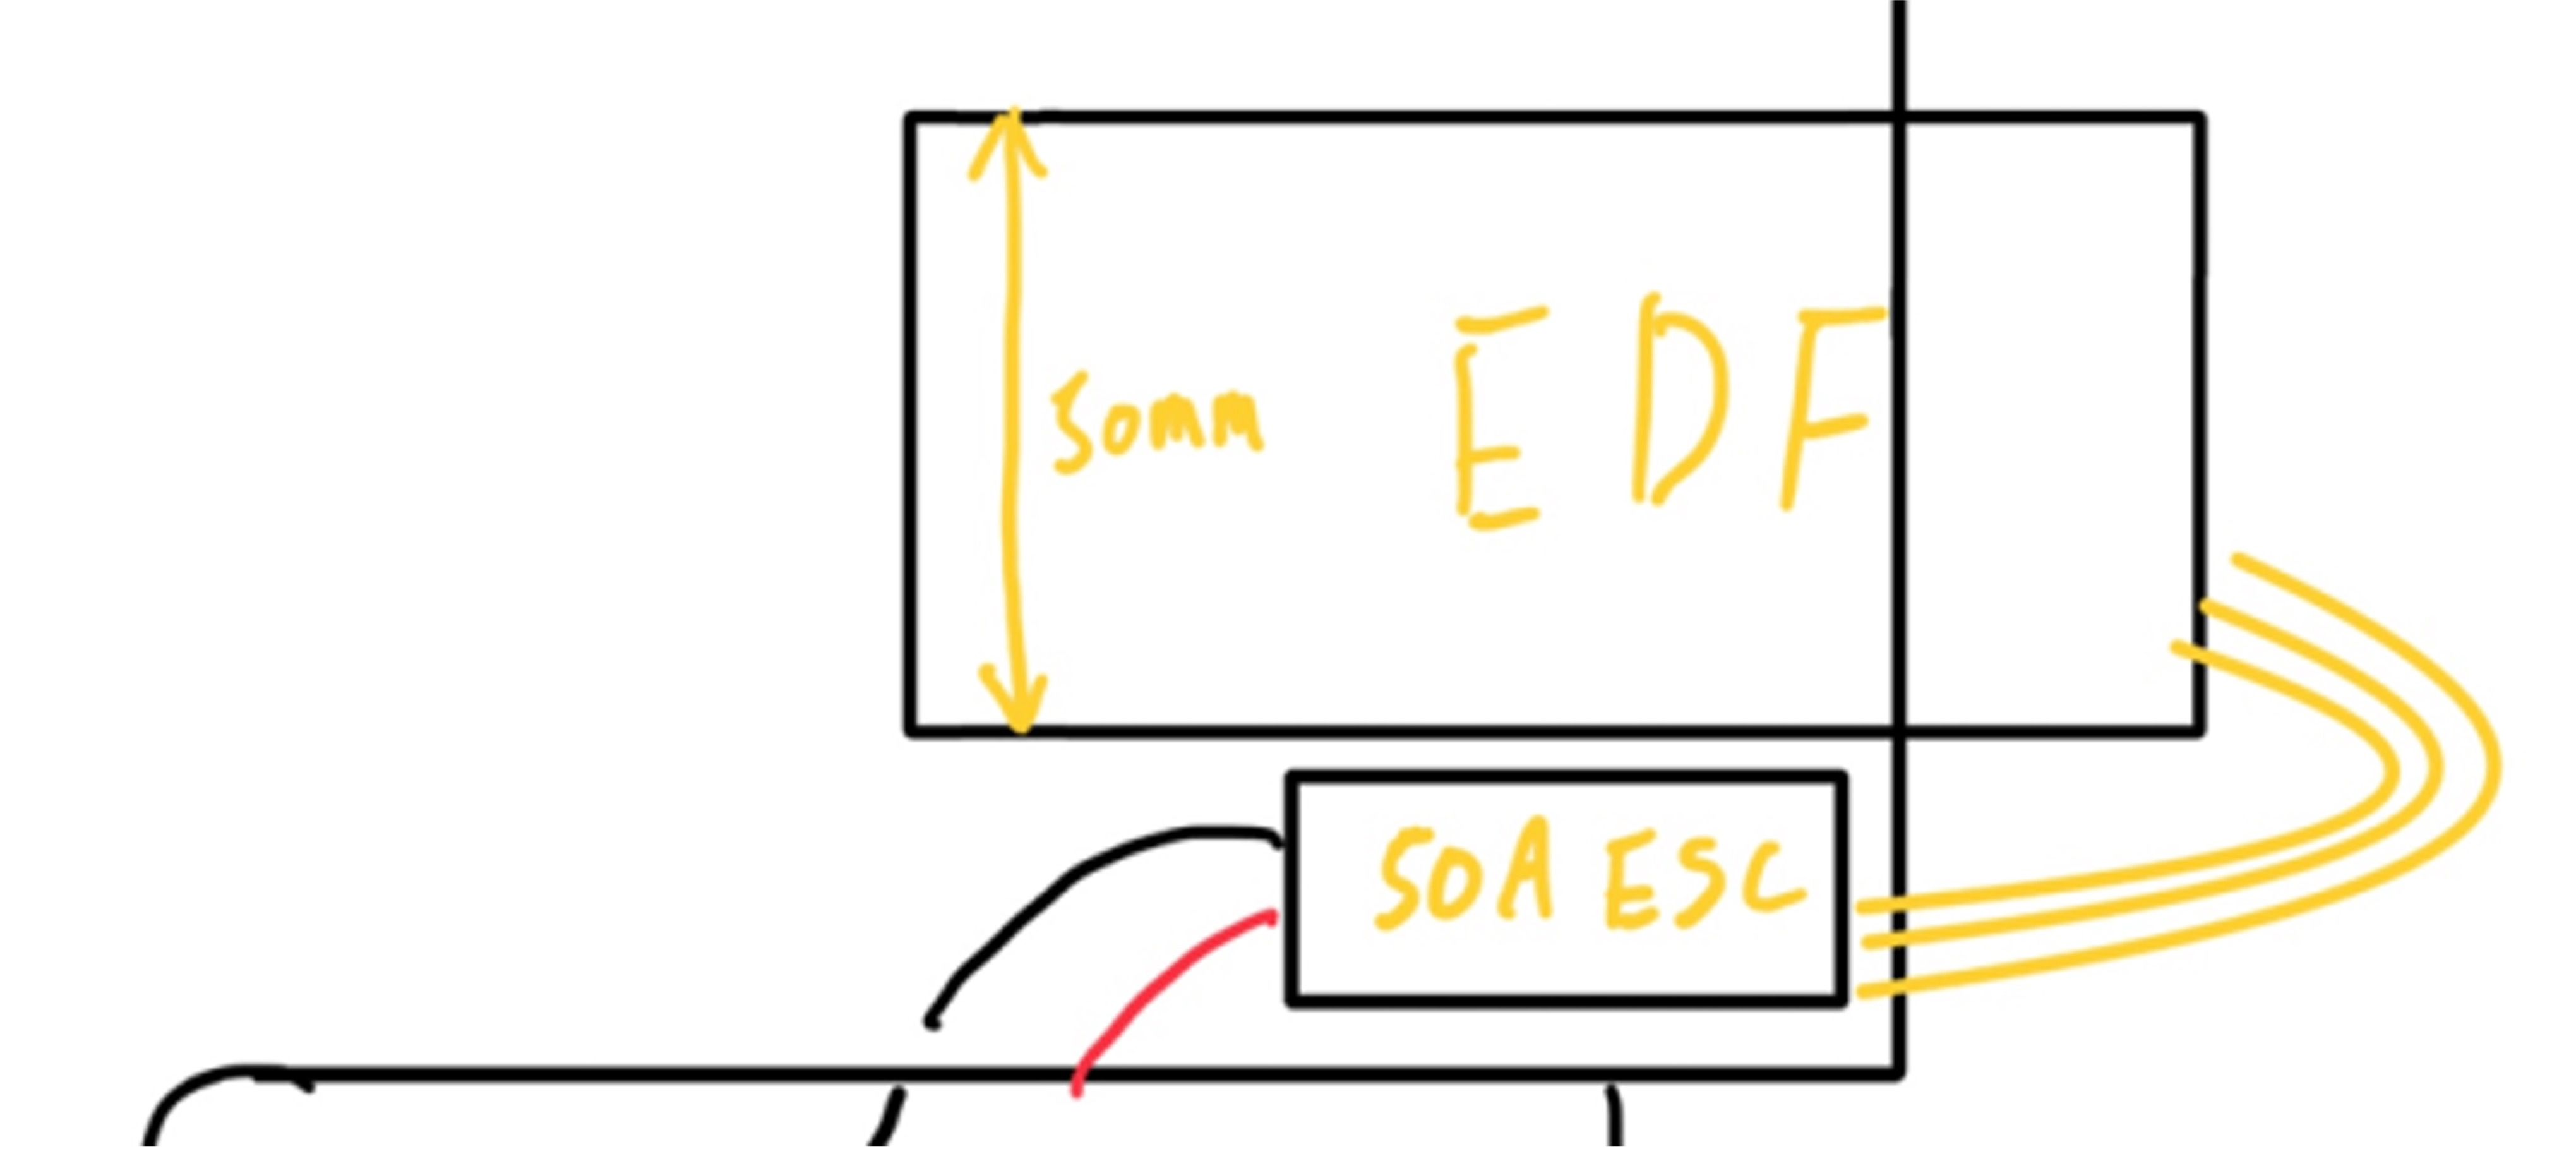
\includegraphics[width=0.7\textwidth]{5.jpg}     %圖片檔案名稱
    \caption{自動控制系統草圖}    %圖片檔案名稱
    \label{fig:5}    %為圖片添加標籤
    %如\ref{fig:example1}所示
\end{figure}
%==============================內文==============================

\subsubsection{輪椅草圖}
%==============================內文==============================
\hspace{2em}
\begin{figure}[H]
    \centering
    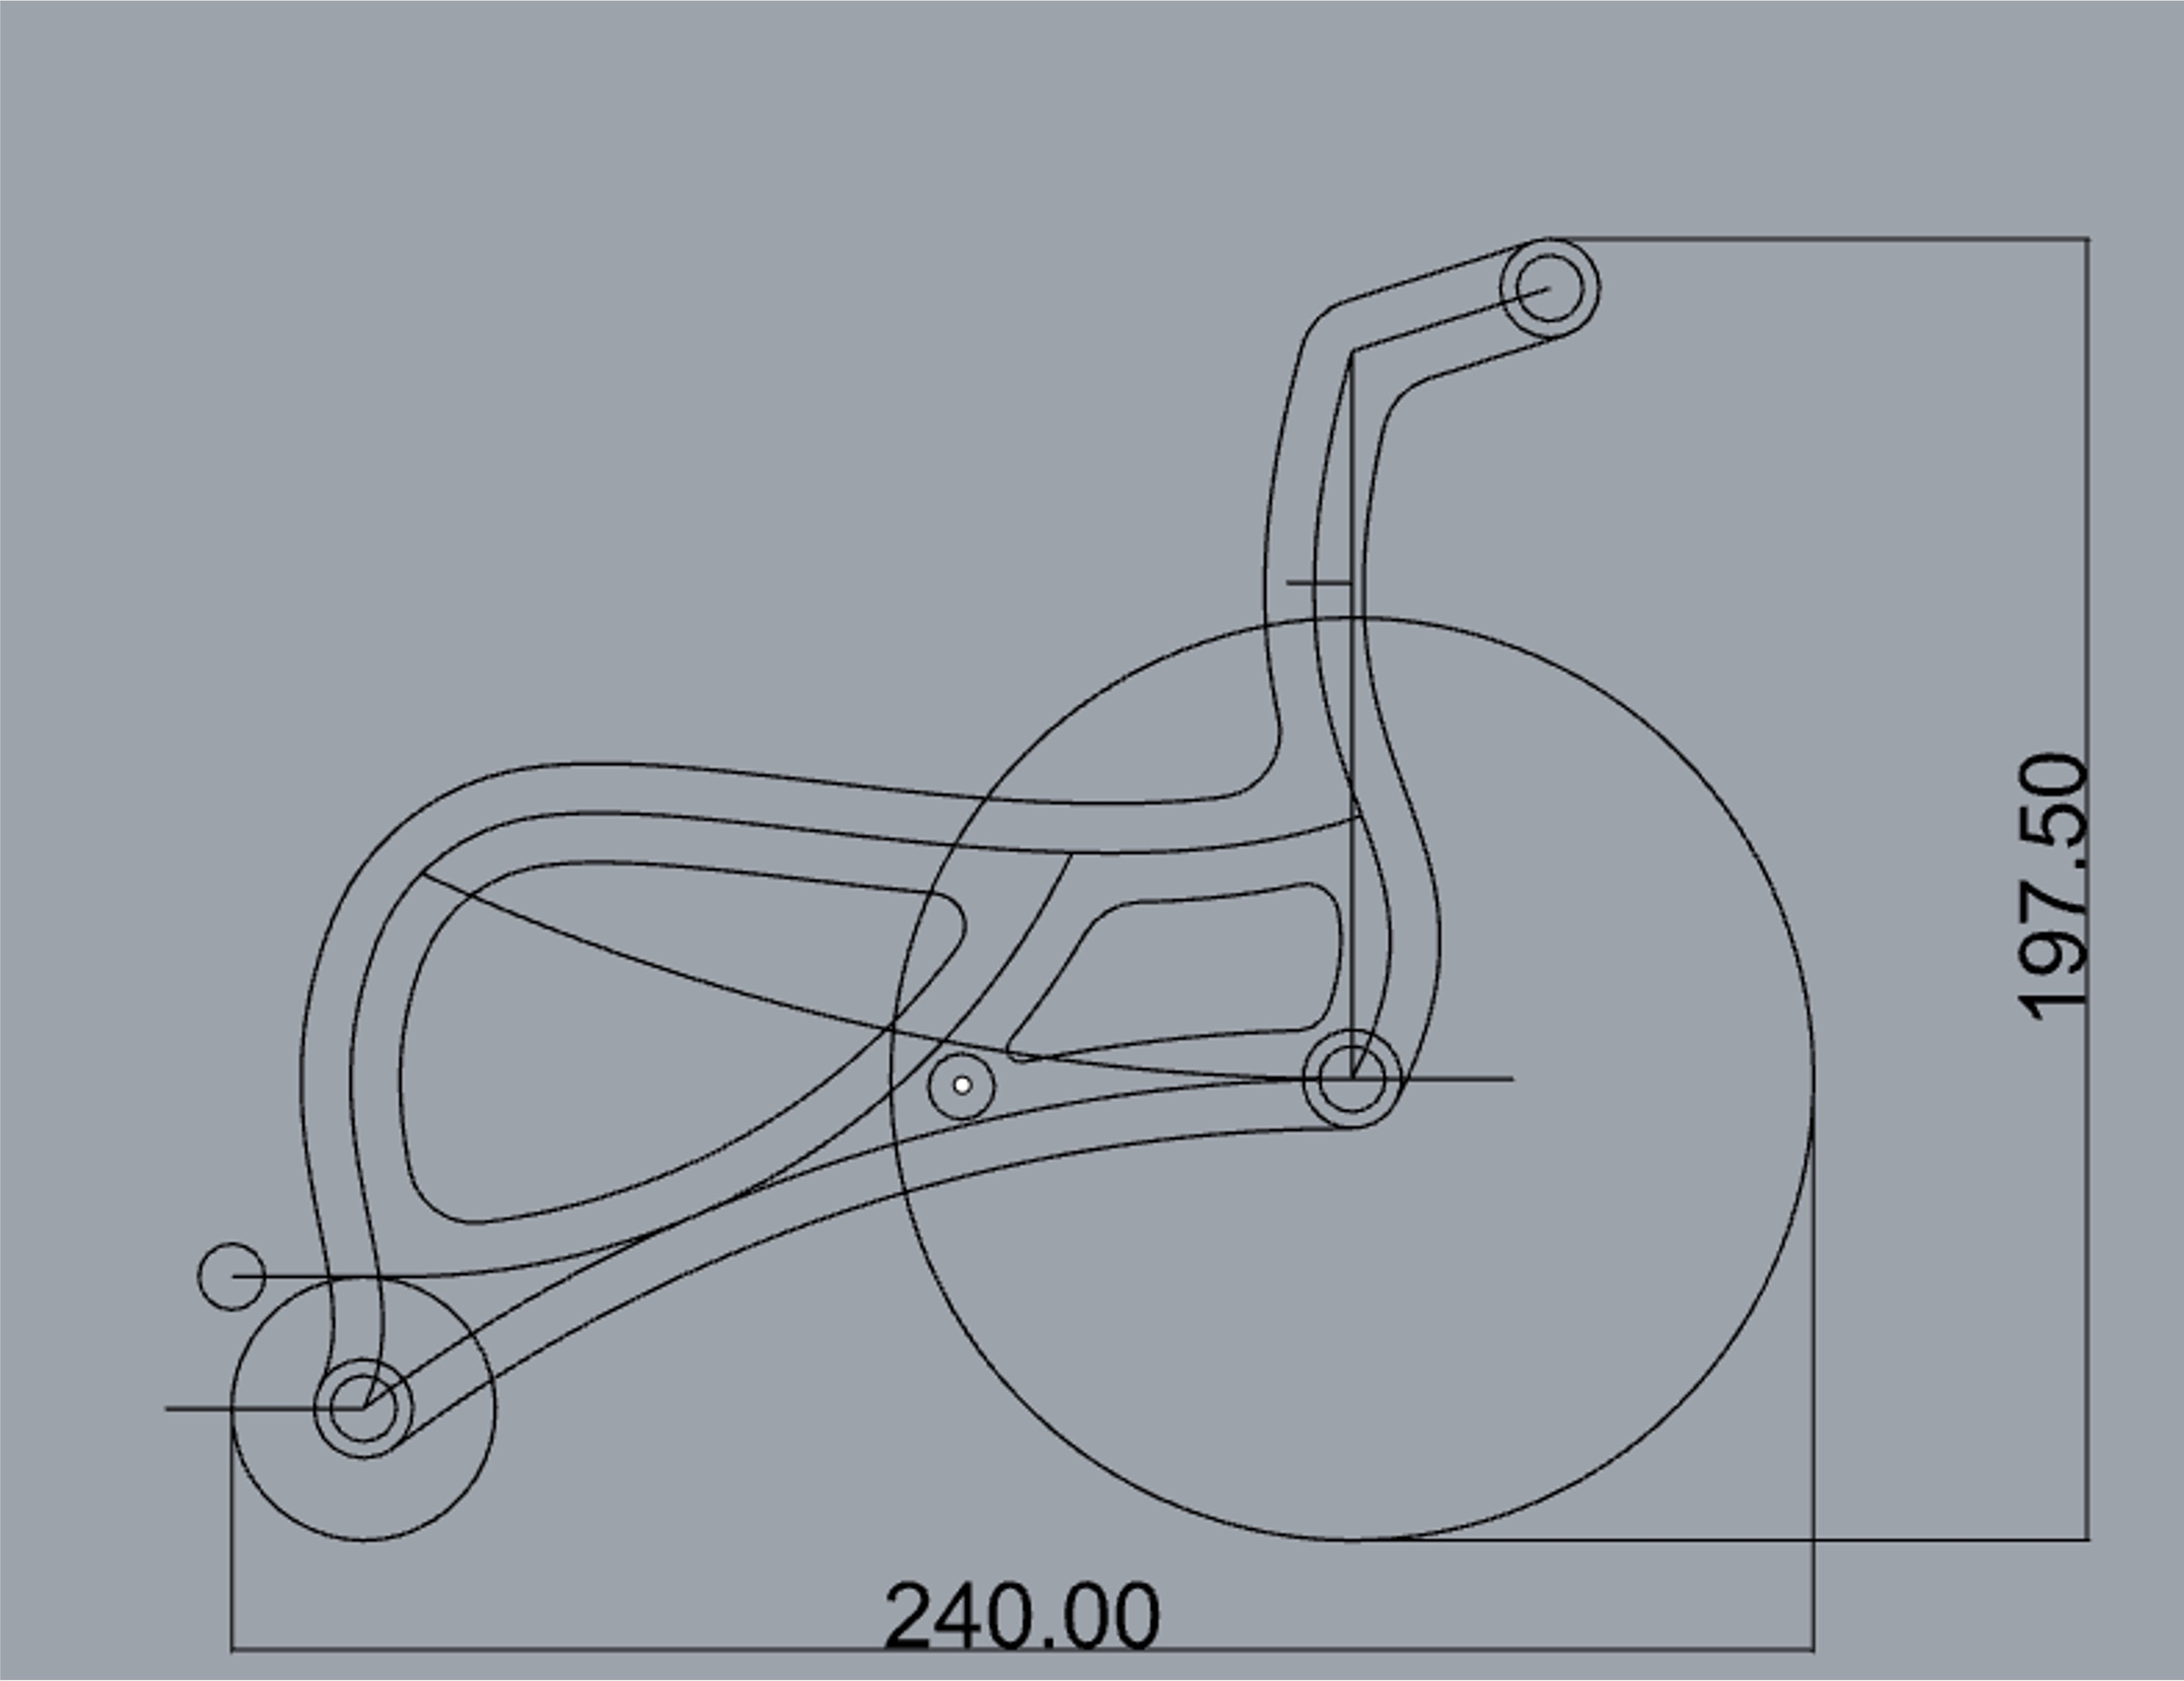
\includegraphics[width=0.6\textwidth]{6.jpg}     %圖片檔案名稱
    \caption{輪椅草圖}    %圖片檔案名稱
    \label{fig:6}    %為圖片添加標籤
    %如\ref{fig:example1}所示
\end{figure}
%==============================內文==============================

\subsubsection{硬體架構}
%==============================內文==============================
\hspace{2em}本系統以 Raspberry Pi 3B+ 作為核心控制器,負責影像處理、邏輯判斷與用戶介面等高層運算任務。考量到 Raspberry Pi 使用 3.3V TTL 電平,而 Arduino 採用 5V TTL,因此選擇透過 UART 通訊介面 進行資料交換,可有效簡化接線、降低相容性問題,並避免馬達啟停時瞬間電流對主控板造成干擾。

在系統架構中,所有感測元件(如攝影機、IMU、按鍵等)皆直接連接至 Raspberry Pi,由其統一進行資料擷取與分析;而 Arduino 則專職負責執行層控制任務,包括:
控制 EDF 風扇啟動與停止與控制伺服馬達與四連桿機構實現轉向動作。
此種分層架構不僅有助於程式模組化管理,也能提升系統穩定性與維護彈性。

\begin{figure}[H]
    \centering
    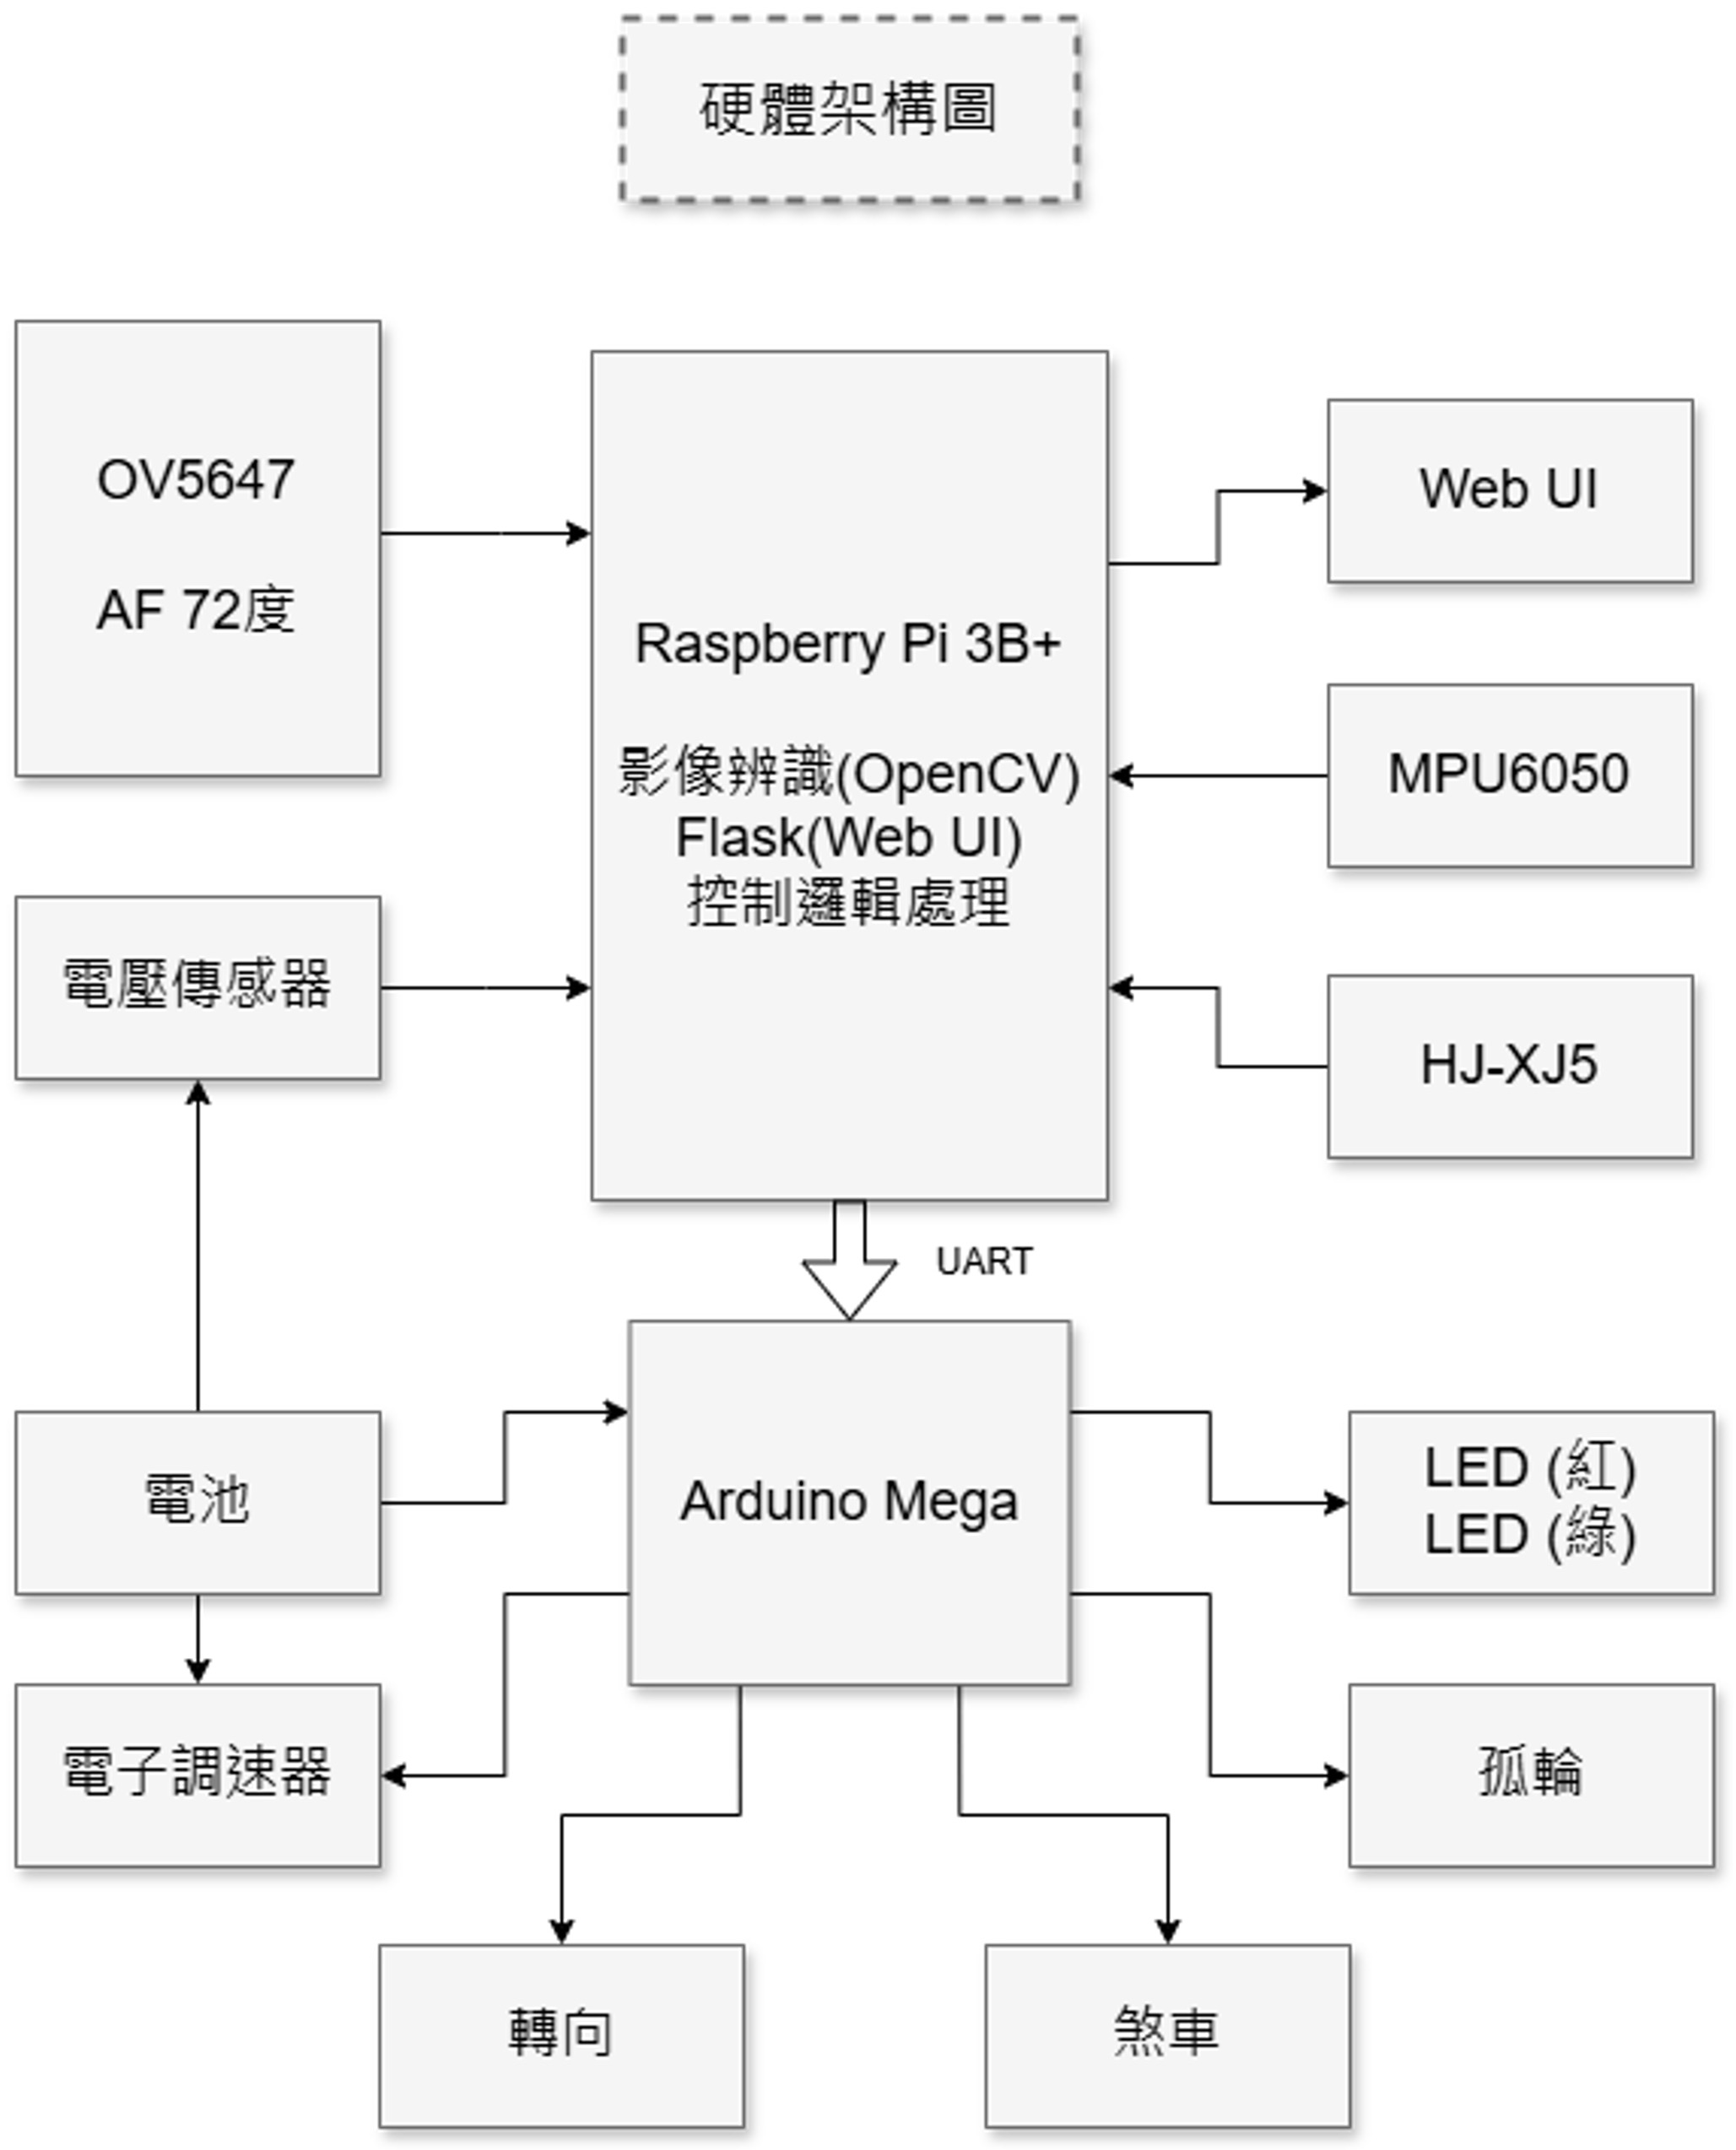
\includegraphics[width=0.6\textwidth]{7.jpg}     %圖片檔案名稱
    \caption{硬體架構圖}    %圖片檔案名稱
    \label{fig:7}    %為圖片添加標籤
    %如\ref{fig:example1}所示
\end{figure}
%==============================內文==============================
\subsection{風扇與葉片設計} 

\subsubsection{動力來源}
%==============================內文==============================
\hspace{2em}風扇通常由電動機(馬達)驅動,將電能轉換為機械能,使葉片旋轉。
%==============================內文==============================

\subsubsection{風扇設計}
%==============================內文==============================
\hspace{2em}葉片的形狀與角度(攻角)決定了風扇的效率與風量。
葉片旋轉時,根據伯努利原理與動量守恆,空氣從低壓區流向高壓區,形成風流。
葉片數量、長度與彎曲度也影響氣流模式(軸流、離心或混合流)。
%==============================內文==============================

\subsubsection{葉片設計}
%==============================內文==============================
\hspace{2em}葉片設計包含三部分,葉片數量、葉片形狀和角度、葉片長度與寬度。
葉片數量方面,少葉片(3~5片)適合高速旋轉,風速快,但風壓較低。多葉片(7片以上):提供較高的風壓,適合對抗阻力的應用(如散熱器、空調)。

葉片形狀與角度這方面葉片的攻角(Blade Angle)影響空氣推動力。較大攻角(20~45°)提供較高風壓,但阻力增加,可能降低轉速。較小攻角(10~20°)提升風速,適合低阻力環境。
扭曲葉片,可減少渦流,提高效率。仿生學設計(如模仿鯨魚胸鰭、鷹翼)可減少空氣阻力,提高流動效率。

葉片長度與寬度方面加長葉片可提高風量,但需注意馬達負載。加寬葉片有助於提升風壓,適用於高阻力場景。

我們的設計策略是根據應用需求選擇葉片數量,確保風壓與風量的平衡。
%==============================內文==============================

\subsection{電機與轉速} 
%==============================內文==============================
\hspace{2em}風力大小與轉速成正比需選擇高效能電機,如:無刷直流電機(BLDC):效率高、壽命長,適合高速風扇。感應電機(Induction Motor):適用於大功率風扇。

我們使用的風扇規格如表\ref{tab:fan}所示:
    \begin{table}[H]
        \centering
        \caption{風扇規格}
        \vspace{6pt} % 增加空格
        \label{tab:fan}
        \begin{tabular}{ll}
            \toprule
            \textbf{項目} & \textbf{規格} \\
            \midrule
            風扇直徑 \(D\) & \(50\,\mathrm{mm} = 0.05\,\mathrm{m}\) \\
            葉片數 & 11 \\
            EDF 型號 & \(50\,\mathrm{mm}\,EDF\) \\
            馬達 KV 值 & \(4500\,\mathrm{KV}\)\\
            電池電壓 & \(3S = 11.1\,\mathrm{V}\)\\
            \bottomrule
        \end{tabular}
        %如\ref{tab:TT2}所示
    \end{table}

    理論轉速計算如下:
    \begin{align}
        \text{RPM} &= KV \times V = 4500 \times 11.1  \label{eq:1}
        \\
        &= 49950\text{RPM} \nonumber
        %式\ref{eq:2}
    \end{align}

    風扇出口速度計算式\ref{eq:2},$V_e$為出口速度,$\text{RPM}$為馬達轉速,$\text{D}$為風扇直徑,$K_e$為出口速度係數(通常介於0.1至0.2)。
    \begin{align}
        V_e &= K_e \cdot \text{RPM} \cdot D  \label{eq:2}
        \\
        &= 0.1 \cdot 49950 \cdot 0.05  \nonumber
        \\
        &= 249.75 m/s \nonumber
        %式\ref{eq:2}
    \end{align}
%==============================內文==============================

\subsection{風道與結構設計} 
\subsubsection{風扇外框與導流設計}
%==============================內文==============================
\begin{itemize}
    \item 加裝導風罩(Shroud)可集中氣流,提高風速與效率。
    \item 收縮式進風口(如噴嘴設計)可增加流速,提高出風動能。
    \item 擾流板(Guide Vanes)可減少渦流,提升氣流穩定度。
\end{itemize}
%==============================內文==============================

\subsubsection{風扇類型選擇}
%==============================內文==============================
\begin{itemize}
    \item 軸流風扇(Axial Fan)適合長距離送風(如電腦散熱、風扇塔)。
    \item 離心風扇(Centrifugal Fan)適合高風壓應用(如空調、渦輪增壓器)。

    \item 混流風扇(Mixed Flow Fan)結合兩者優勢,提高風壓與風量。
\end{itemize}
%==============================內文==============================

\subsubsection{風扇導流罩}
%==============================內文==============================
\hspace{2em}主要作用是提升風扇的推力與效率,其原理涉及氣流控制、減少渦流、提高風壓與風速。
導流罩的幾個關鍵機制為增加氣流速度(噴射效應)與減少渦流與能量損失。
風扇在運轉時,葉片末端(特別是無外框的風扇)會產生強烈的端部渦流(Tip Vortex)會導致氣流擾動降低風壓與能量損耗使推力下降。

導流罩可封閉葉片端部,減少氣流洩漏,進而提高風扇效率。目前打算設計變截面導流罩(Converging Nozzle),入口與出口皆有變化,可提升氣流效率,減少能量損耗。
%==============================內文==============================

\subsection{空氣動力學設計} 
%==============================內文==============================
\begin{itemize}
    \item 降低車身阻力(Drag Reduction)
    \item 流線型設計,避免平直表面,減少風阻
    \item 使用導流罩(Shroud)引導風扇氣流,提高推進效率
    \item 穩定性
    \item 風扇的反作用力可能影響車輛平衡,需要考慮重心設計
    \item 若車輛速度高,可加裝尾翼,減少側風影響
\end{itemize}

推力計算如下所示,$\rho = 1.225(kg/m^3)$、$V_i =0$、$D=0.05(m)$:
\begin{align}
    T &= \dot{m} \cdot (V_e - V_i) \label{eq:thrust_formula} 
    \\
    &= \rho \cdot A \cdot V_e \cdot (V_e - V_i)   \nonumber
    \\
    &= \rho \cdot \frac{1}{4} \cdot D^2\cdot \pi \cdot V_e \cdot (V_e - V_i)   \nonumber
    \\
     &=1.225\times \frac{\pi}{4}\times 0.05^2 \times249.75\times(249.75-0) \nonumber
    \\
    T &= 150.0296(N)    \nonumber
\end{align}

當汽車行駛時,會受到空氣阻力,$CD$為阻力係數,$\rho$為空氣密度,$A$車體迎風面,$v$為車速,其公式如式\ref{eq:3}。
\begin{align}
    FD=\frac{1}{2}CDv^{2}\rho A  \label{eq:3}
    %式\ref{eq:2}
\end{align}
降低空氣阻力的方法包含流線型車身設計(減少迎風面積)、降低車輛高度(減少底部亂流)、使用導流板(減少渦流與尾流)。

汽車在高速行駛時,車身可能會產生升力(Lift),導致車輛不穩定而F1賽車則透過空氣動力學產生下壓力(Downforce)來增加抓地力。升力公式如式\ref{eq:3}。
\begin{align}
    FL=\frac{1}{2}CLv^{2}\rho A  \label{eq:4}
    %式\ref{eq:2}
\end{align}
減少升力的方法包含加裝尾翼(Spoiler)、底部擴散器(Diffuser)、前擾流板(Front Splitter)。
加裝尾翼可改變氣流方向,增加下壓力。底部擴散器,增加地面效應,減少氣流擾動。前擾流板可提升車頭穩定性。

風扇驅動車是靠風扇推進,需要考慮:

\begin{enumerate}
    \item 風扇的推力與效率 : 使用導流(Shroud)來提高推力。
    \item 車身形狀 : 流線型設計可減少阻力,讓風扇推動更有效。
    \item 尾流管理 : 避免車後氣流分離,降低拖曳力,提高速度。
\end{enumerate}
%==============================內文==============================

\subsection{演算法設計} 
%==============================內文==============================
\hspace{2em}循線演算法將結合影像偵測與模糊控制實現,並包含預處理、偵測、模糊控制三部分。演算法流程圖如\ref{fig:9}圖所示。
\begin{figure}[H]
    \centering
    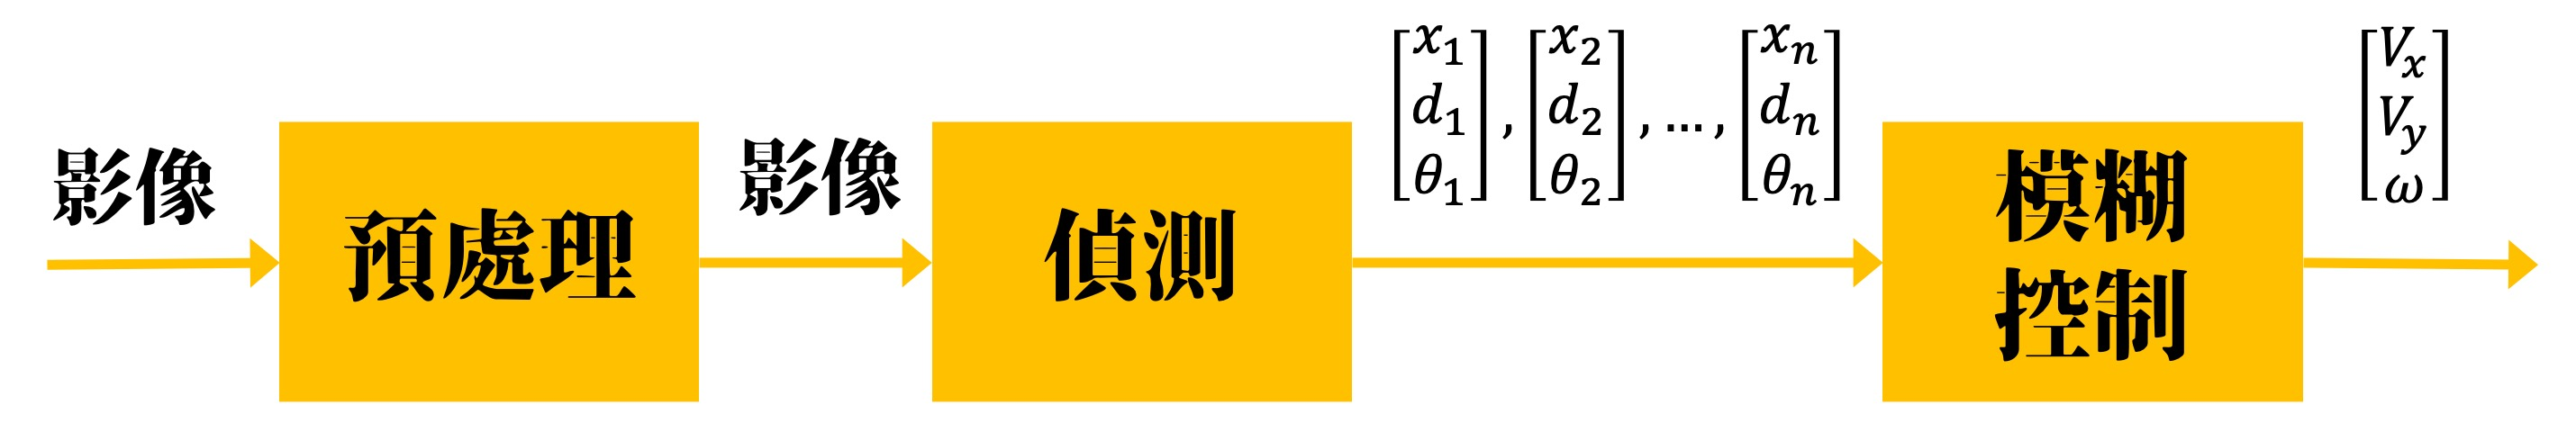
\includegraphics[width=0.9\textwidth]{9.jpg}     %圖片檔案名稱
    \caption{影像循線演算法流程圖}    %圖片檔案名稱
    \label{fig:9}    %為圖片添加標籤
    %如\ref{fig:example1}所示
\end{figure}

演算法的輸入為影像,演算法的輸出為車輛為$V_{x}$、$V_{y}$與$\omega$,定義如下圖\ref{fig:10}所示。
\begin{figure}[H]
    \centering
    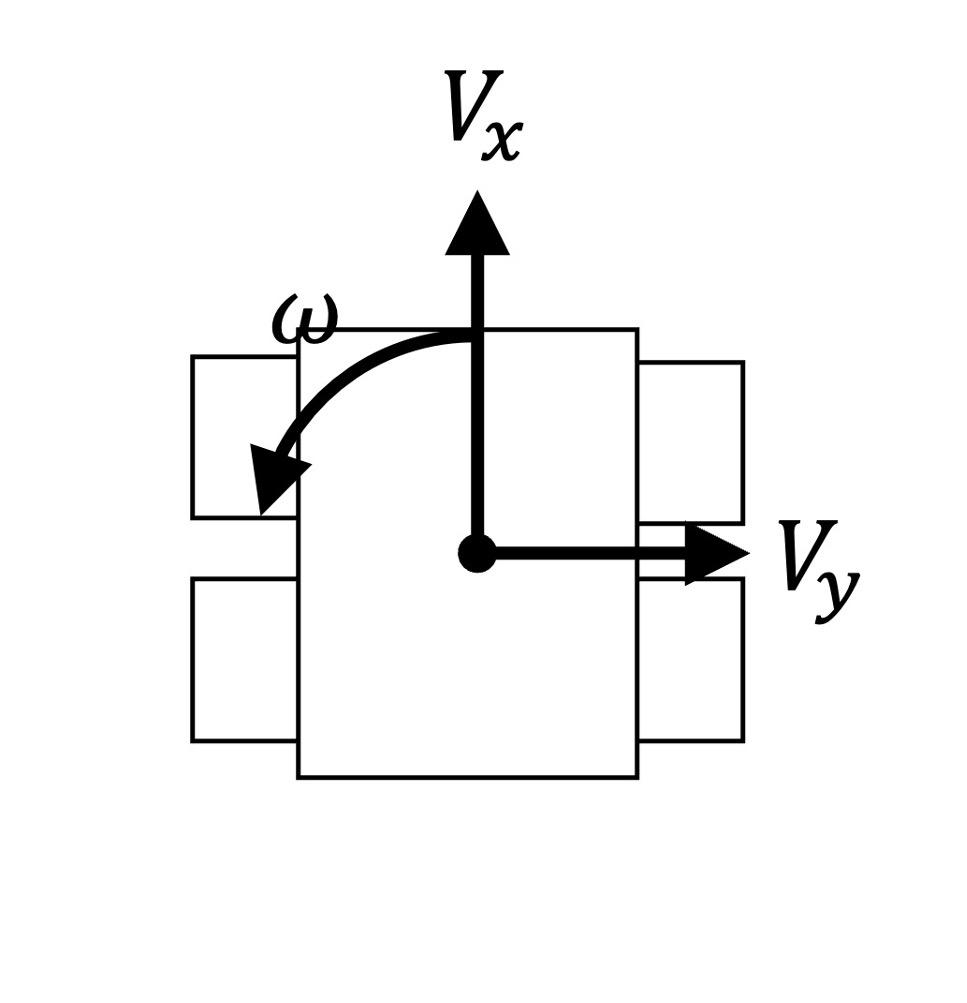
\includegraphics[width=0.5\textwidth]{10.jpg}     %圖片檔案名稱
    \caption{車輛速度定義}    %圖片檔案名稱
    \label{fig:10}    %為圖片添加標籤
    %如\ref{fig:example1}所示
\end{figure}
%==============================內文==============================

\subsubsection{預處理}
%==============================內文==============================
\hspace{2em} 此部分要將影像拍攝影像處理成可供影像偵測之影像,包括透視變換、灰階處理、高斯模糊、二值化、Canny邊緣偵測五步驟,將接收到的影像進行處理,提供後續偵測使用。

\begin{figure}[H]
    \centering
    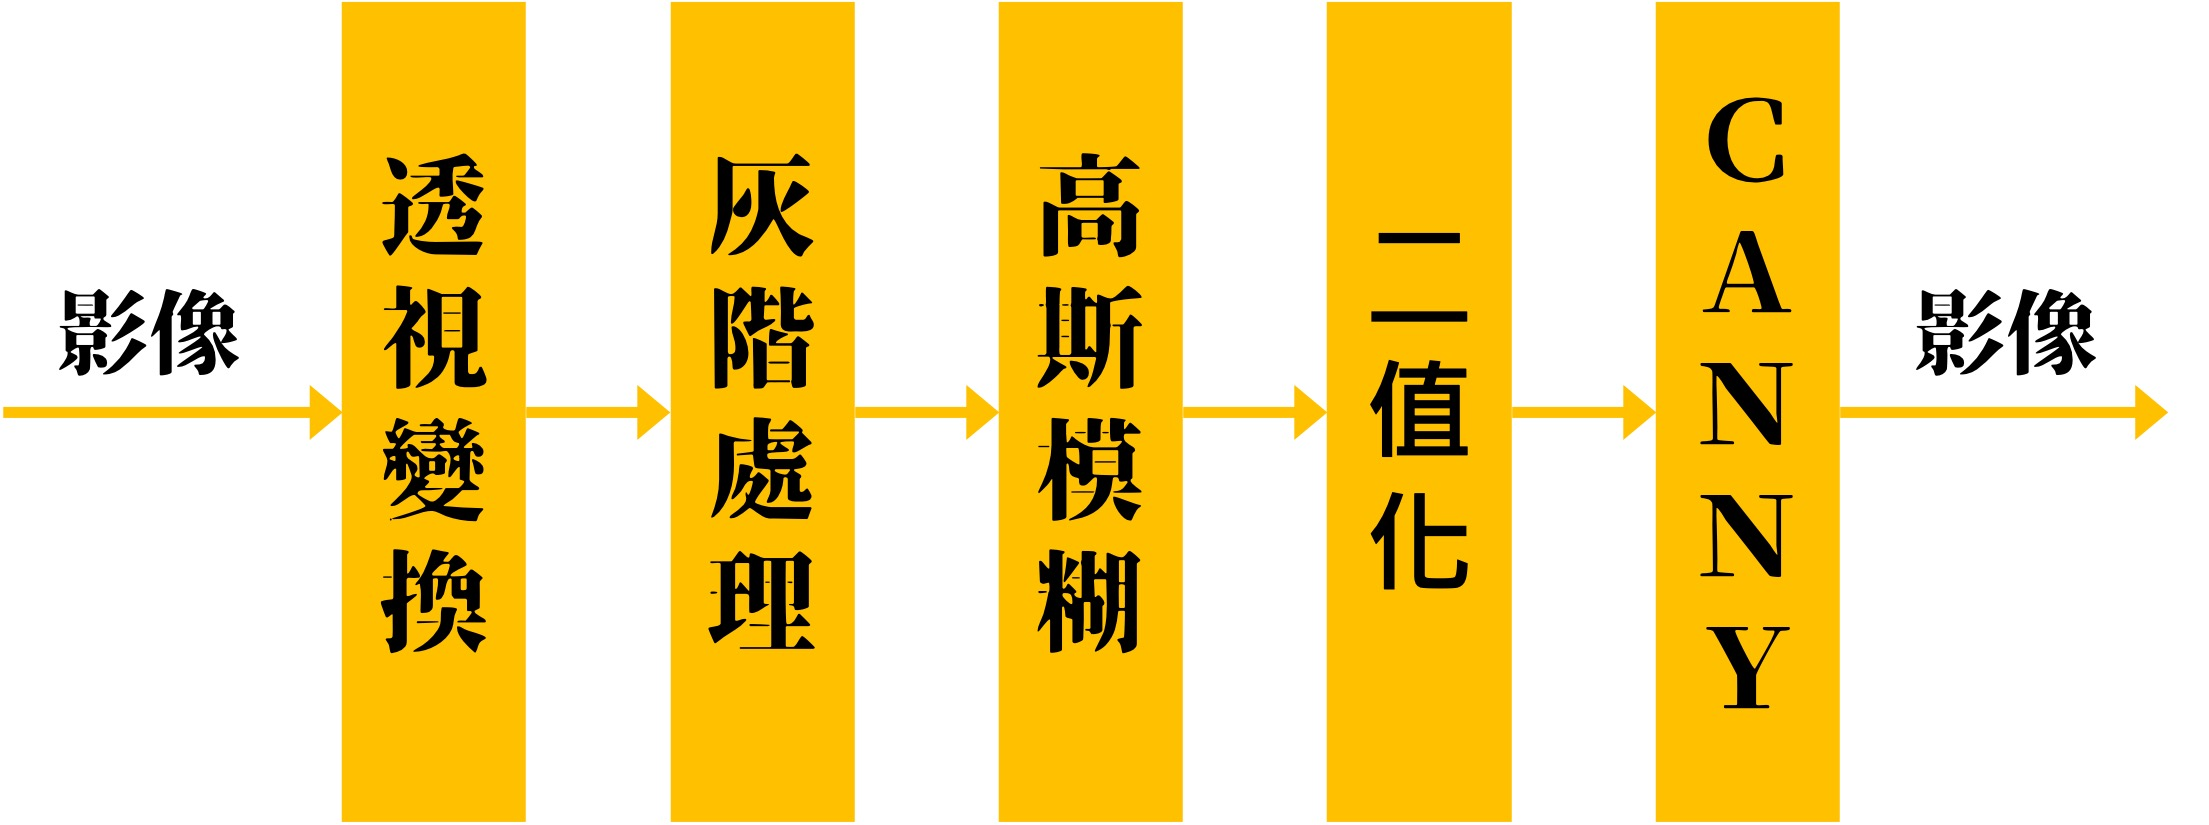
\includegraphics[width=0.7\textwidth]{11.jpg}     %圖片檔案名稱
    \caption{影像預處理流程圖}    %圖片檔案名稱
    \label{fig:11}    %為圖片添加標籤
    %如\ref{fig:example1}所示
\end{figure}

首先,對捕獲的影像進行透視變換,將影像轉換為以車輛為原點的二維座標系統,這樣有助於確定車輛與道路的相對位置,並為後續的計算提供準確的基準。公式\ref{eq:fy}及示意圖(如圖\ref{fig:15}、圖\ref{fig:14}所示)如下:
\begin{align}
    \begin{bmatrix}
        x_{car}   \\
        y_{car}   
    \end{bmatrix} 
     &=f(
     \begin{bmatrix}
        x       \\
        y       
    \end{bmatrix} 
    ,W,H,\theta_{camera},HFOV,WFOV)
    \label{eq:xcarycar}
\end{align}
\begin{figure}[H]
    \centering
    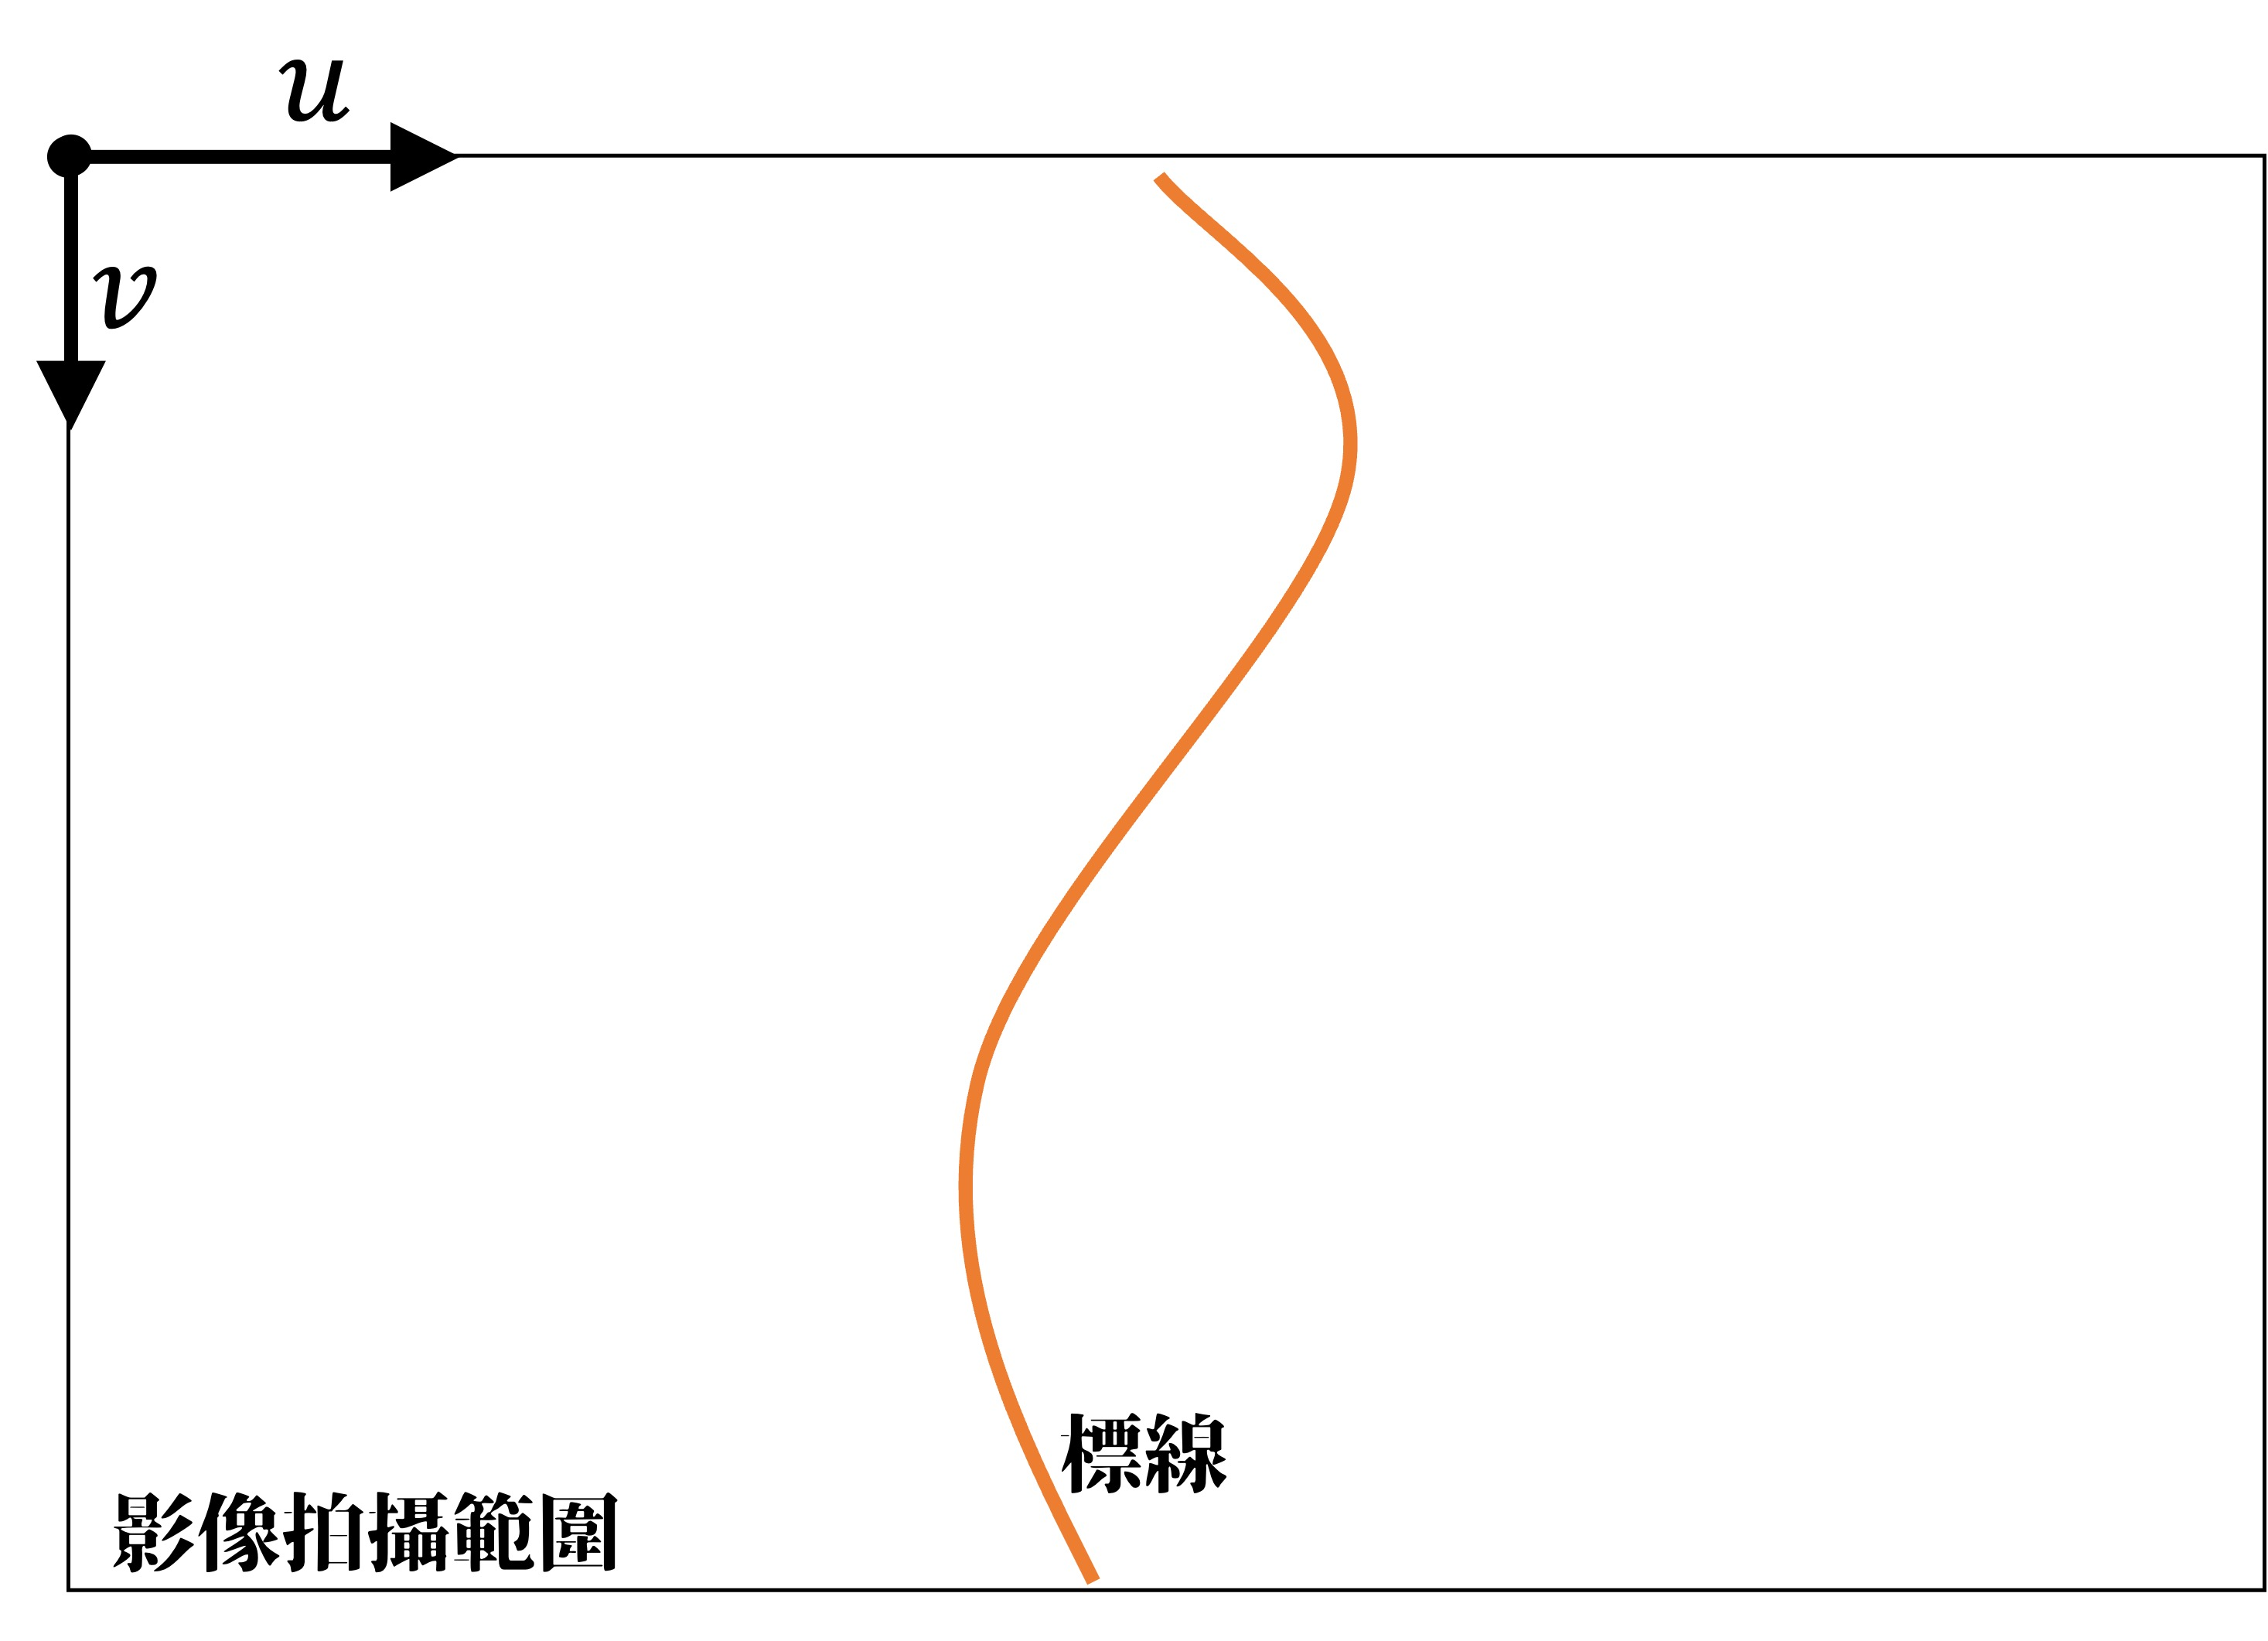
\includegraphics[width=0.7\textwidth]{15.jpg}     %圖片檔案名稱
    \caption{相機拍攝之原始影像}    %圖片檔案名稱
    \label{fig:15}    %為圖片添加標籤
    %如\ref{fig:example1}所示
\end{figure}
\begin{figure}[H]
    \centering
    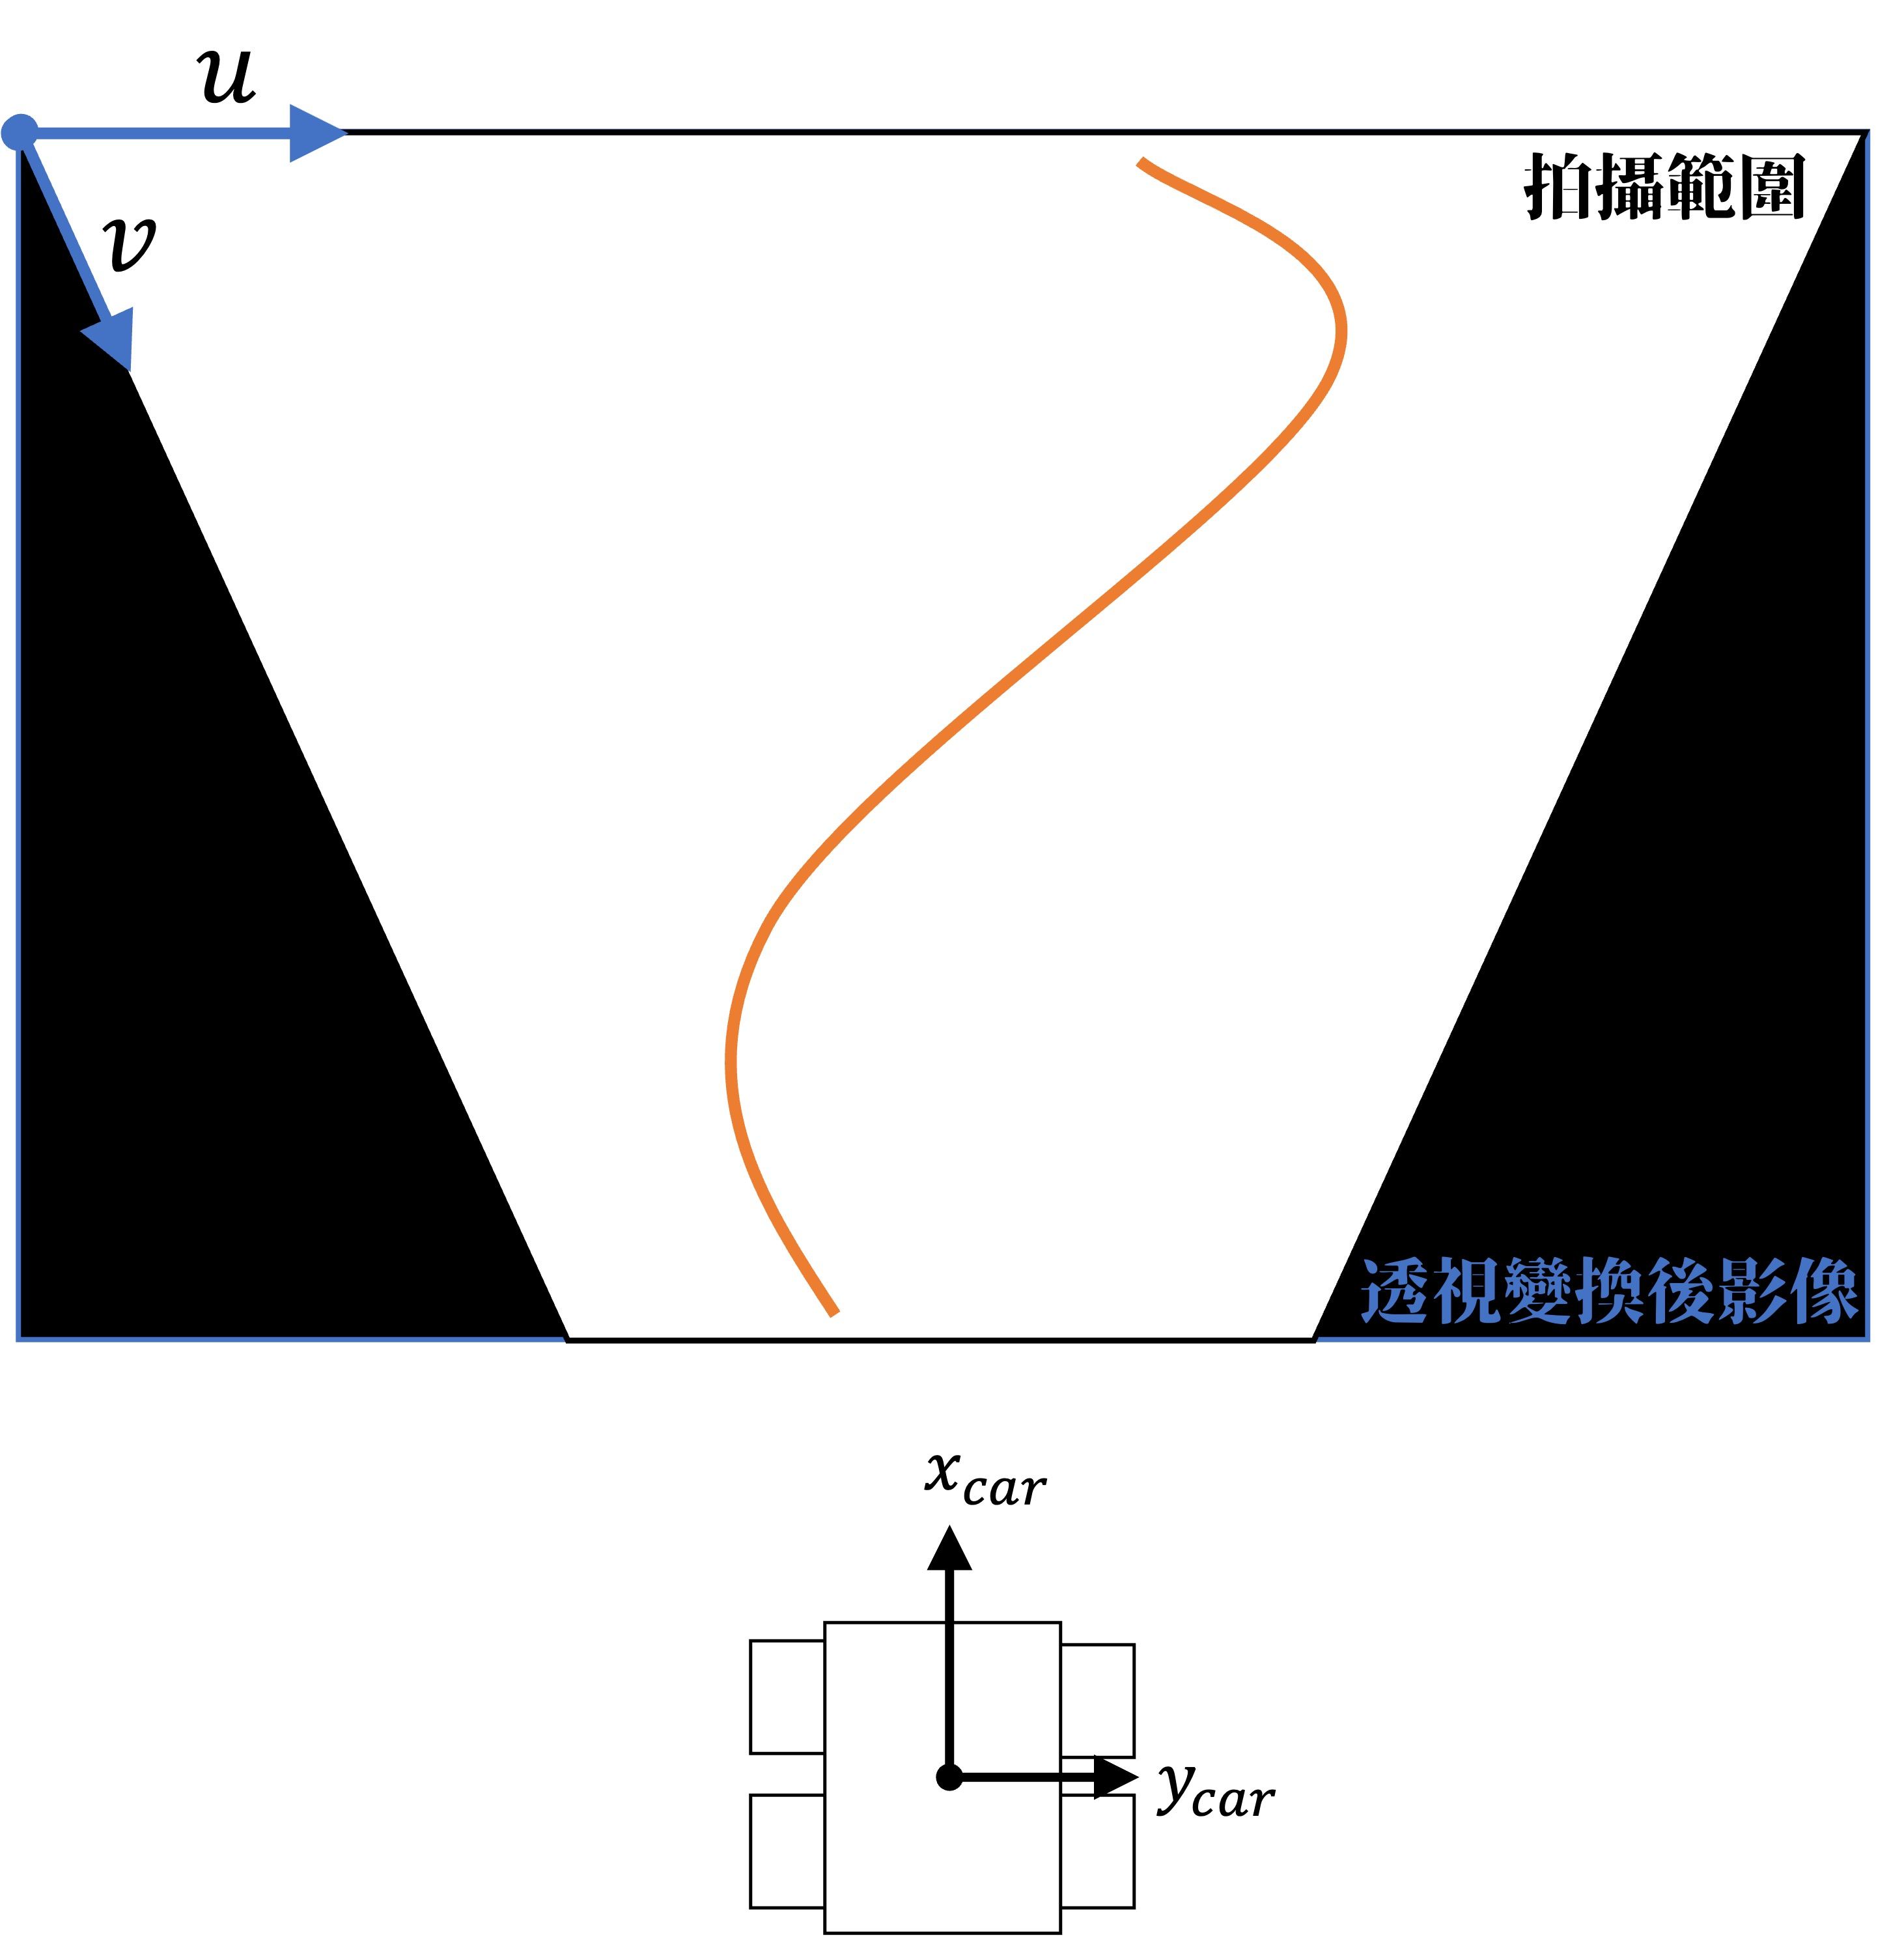
\includegraphics[width=0.7\textwidth]{14.jpg}     %圖片檔案名稱
    \caption{車輛座標系與像素坐標系關係之示意圖}    %圖片檔案名稱
    \label{fig:14}    %為圖片添加標籤
    %如\ref{fig:example1}所示
\end{figure}
將利用鏡頭往斜下的角度拍攝。採用逆透視變換(Inverse Perspective Mapping,IPM)\cite{lin_2001}\cite{bertozz1998stereo}\cite{mallot1991inverse}技術處理影像,可以將像素座標轉換為地面座標,取得影像中精確的距離。

透視變換的核心在於去除透視效應,以便將影像中的道路線條轉換為平行的直線。這樣的變換有助於車輛識別路徑,使後續演算法能夠更容易地進行路徑規劃與車道偵測。

首先將影像像素座標系$(u,v)$轉換為圖像座標系$(x,y)$。
加入相機的水平視角$HFOV$與相機的垂直視角$VFOV$、相機俯仰角$\theta_{camera}$,將圖像座標轉換為相機座標$(x_{camera},y_{camera},z_{camera})$。
接著將相機座標系轉換為車輛標系$(x_{car},y_{car},z_{car})$,以取得拍攝影像中內容物與車輛之相對位置。流程圖如下:
\begin{figure}[H]
    \centering
    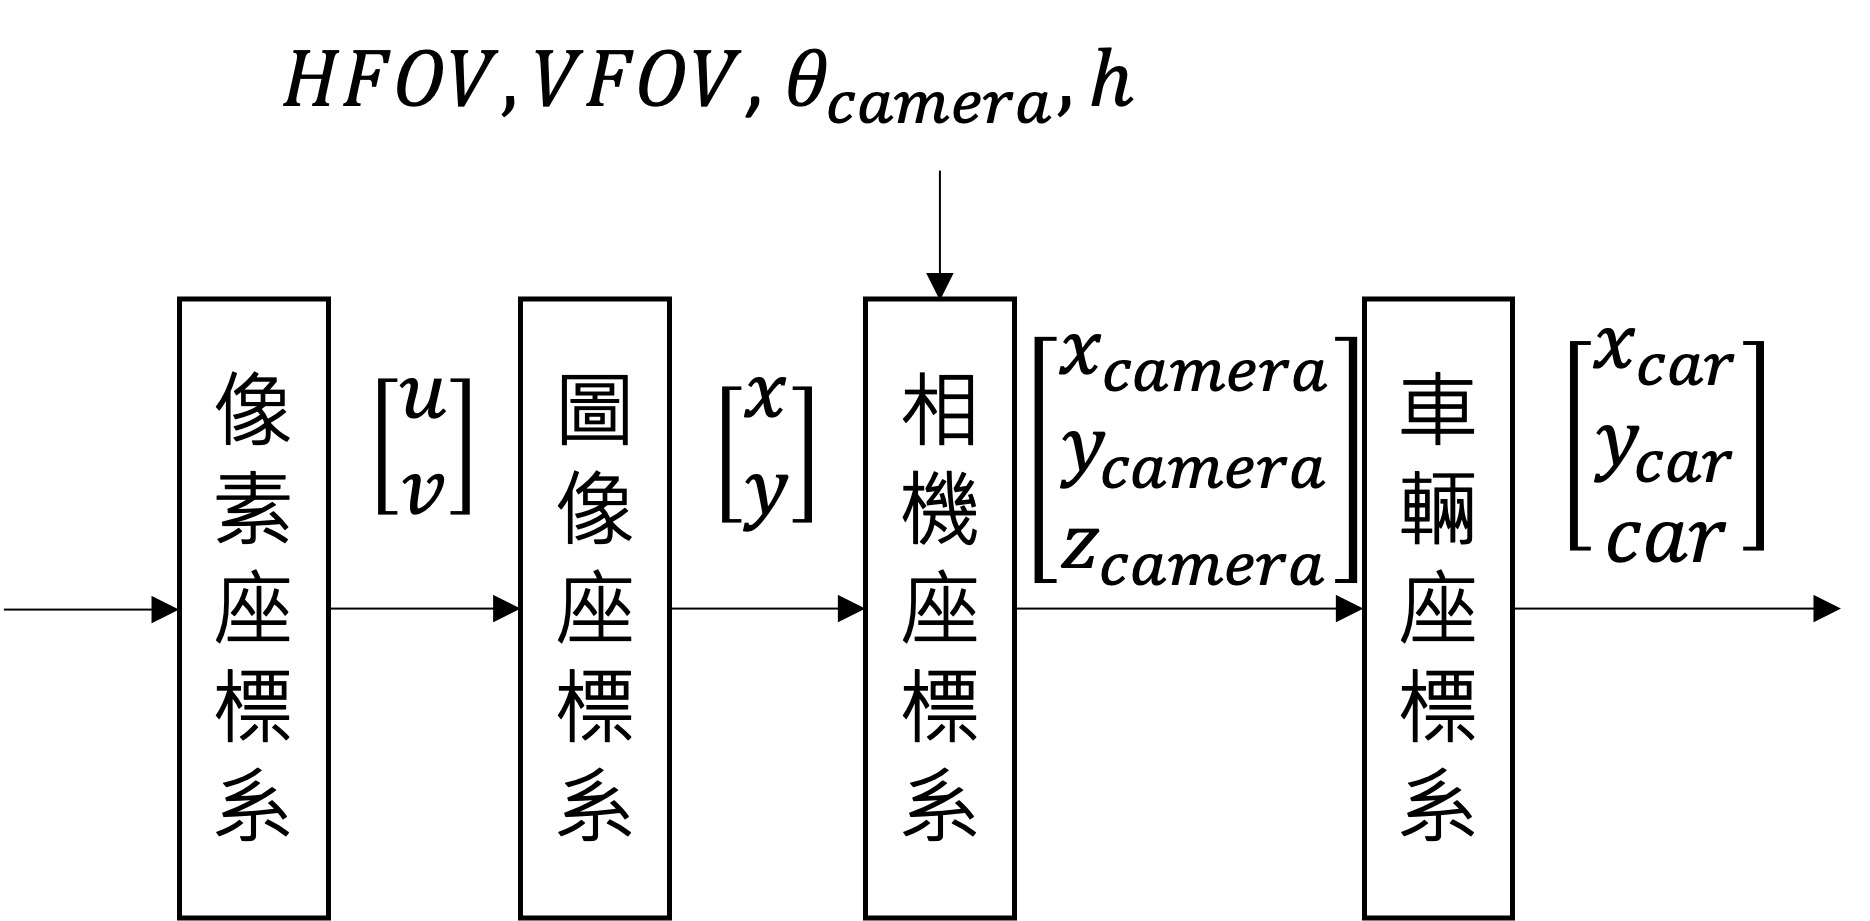
\includegraphics[width=0.7\textwidth]{12.jpg}     %圖片檔案名稱
    \caption{透視變換流程圖}    %圖片檔案名稱
    \label{fig:12}    %為圖片添加標籤
    %如\ref{fig:example1}所示
\end{figure}
將像素座標轉換為無人機相對於地平面的世界座標時,過程涉及相機的內參矩陣$K$、旋轉矩陣$R$以及相機高度$h$。要算相機的內參矩陣首先需得出影像的水平焦距$f_{x}$、影像的垂直焦距$f_{y}$和影像的中心座標$(c_x,c_y)$。

影像的水平焦距$f_{x}$公式如式(\ref{eq:fx}),W為影像的寬度,HFOV為相機的水平視角。
影像的垂直焦距$f_{y}$公式如式(\ref{eq:fy}),H為影像的寬度,VFOV為相機的垂直視角。
\begin{align}
    f_{x}=\frac{W}{2\cdot\tan\left(\frac{HFOV}{2}\right)}
    \label{eq:fx}
    \\
    f_{y}=\frac{H}{2\cdot\tan\left(\frac{VFOV}{2}\right)}
    \label{eq:fy}
\end{align}

影像的中心座標$(c_x,c_y)$公式如式(\ref{eq:cx})、式(\ref{eq:cy}):
\begin{align}
    c_{x}=\frac{W}{2}
    \label{eq:cx}
    \\
    c_{y}=\frac{H}{2}
    \label{eq:cy}
\end{align}

式(\ref{eq:k})為相機內參矩陣K。
\begin{align}
    K &=
    \begin{bmatrix}
        f_{x}       & 0             & c_{x}     \\
        0           & f_{y}         & c_{y}     \\
        0           & 0             & 1
    \end{bmatrix} 
    \label{eq:k}
\end{align}

旋轉矩陣R用來表示相機相對於世界座標系的旋轉。
此處忽略車輛進行中的晃動。旋轉矩陣R如下:
\begin{align}
    R=&
    \begin{bmatrix}
        1   & 0  & 0 \\
        0   & \cos(\theta_{camera})   & -\sin(\theta_{camera}) \\
        0   & \sin(\theta_{camera})   & \cos(\theta_{camera}) \\
    \end{bmatrix} 
    \label{eq:R2}
\end{align}

將像素座標系$(x,y)$轉換為圖像座標系的公式如式(\ref{eq:xy1}):
\begin{align}
    \begin{bmatrix}
        x       \\
        y    \\
        1        
    \end{bmatrix} 
     &=K^{-1}\cdot
     \begin{bmatrix}
        u       \\
        v       \\
        1        
    \end{bmatrix} 
    \label{eq:xy1}
\end{align}

將圖像座標系轉換為相機座標系的公式如式(\ref{eq:xcyczc}):
\begin{align}
    \begin{bmatrix}
        x_{camera}   \\
        y_{camera}   \\
        z_{camera}        
    \end{bmatrix} 
     &=R\cdot
     \begin{bmatrix}
        x       \\
        y       \\
        1        
    \end{bmatrix} 
    \label{eq:xcyczc}
\end{align}
將相機座標系轉換為車輛座標系$(x_{car},y_{wcar},z_{wcar})$的公式見式式(\ref{eq:xw})、式式(\ref{eq:yw}),此公式即可獲已車輛為原點的座標系統,取得每影像中每一像素與車輛的絕對距離。
\begin{align}
    x_{w}=\frac{x_{c}}{z_{c}}
    \label{eq:xw}\\
    y_{w}=\frac{y_{c}}{z_{c}}
    \label{eq:yw}
\end{align}

灰階處理將彩色影像轉換為灰階影像,這樣能有效減少計算量,同時保留影像的基本結構特徵,便於後續處理。
這樣的轉換方式基於人眼對不同顏色敏感度的權重選擇,使得轉換後的影像仍然保持較高的可辨識度。

高斯模糊用來去除影像中的噪聲,這有助於平滑影像,減少後續處理中的干擾,尤其是在邊緣檢測時。
高斯模糊的公式如下:
\begin{align}
G(x,y) = \frac{1}{2\pi\sigma^2} e^{-\frac{x^2 + y^2}{2\sigma^2}}
\end{align}
其中,$\sigma$ 為標準差,決定模糊的強度。較大的 $\sigma$ 值會導致更強的平滑效果,但可能會模糊掉重要的邊緣資訊。

二值化將影像轉換為二值圖像,即只保留黑白兩種顏色,這有助於強調出車道線等重要特徵,便於後續的分析與處理。
固定閾值法:設定一個固定的閾值 $T$,當像素強度高於 $T$ 時設為白色,否則設為黑色。固定閾值法的公式如下。

\begin{align}
    I_{bin}(x,y) = 
    \begin{cases}
        1, & I(x,y) > T \\
        0, & I(x,y) \leq T
    \end{cases}
\end{align}

最後使用Canny 邊緣偵測來提取影像中的邊緣信息,這有助於識別出車道的邊界或其他障礙物,為自走車的導航提供關鍵信息。
%==============================內文==============================

\subsubsection{偵測}
%==============================內文==============================
\hspace{2em}圖像經過預處理後,接下來的步驟是偵測車道標線,並計算車輛的偏移量與偏移角度。

將首先,從影像中掃描特定的區域,通過檢測這些區域的像素值來獲取相關的幾何特徵。
在偵測車道標線時,並非整張影像都具有相同的重要性,因此可以選擇關鍵區域進行分析。例如,車輛前方的道路中央區域可能包含主要的行駛標線,而影像上方區域則可能包含過多的背景資訊,對偵測無實質幫助。
將使用滑動視窗法,使用固定大小的窗口在影像中移動,對每個區域進行局掃描,以提取潛在的車道標線位置,並將視窗滑動偵測最多白色像素之位置。
\begin{figure}[H]
    \centering
    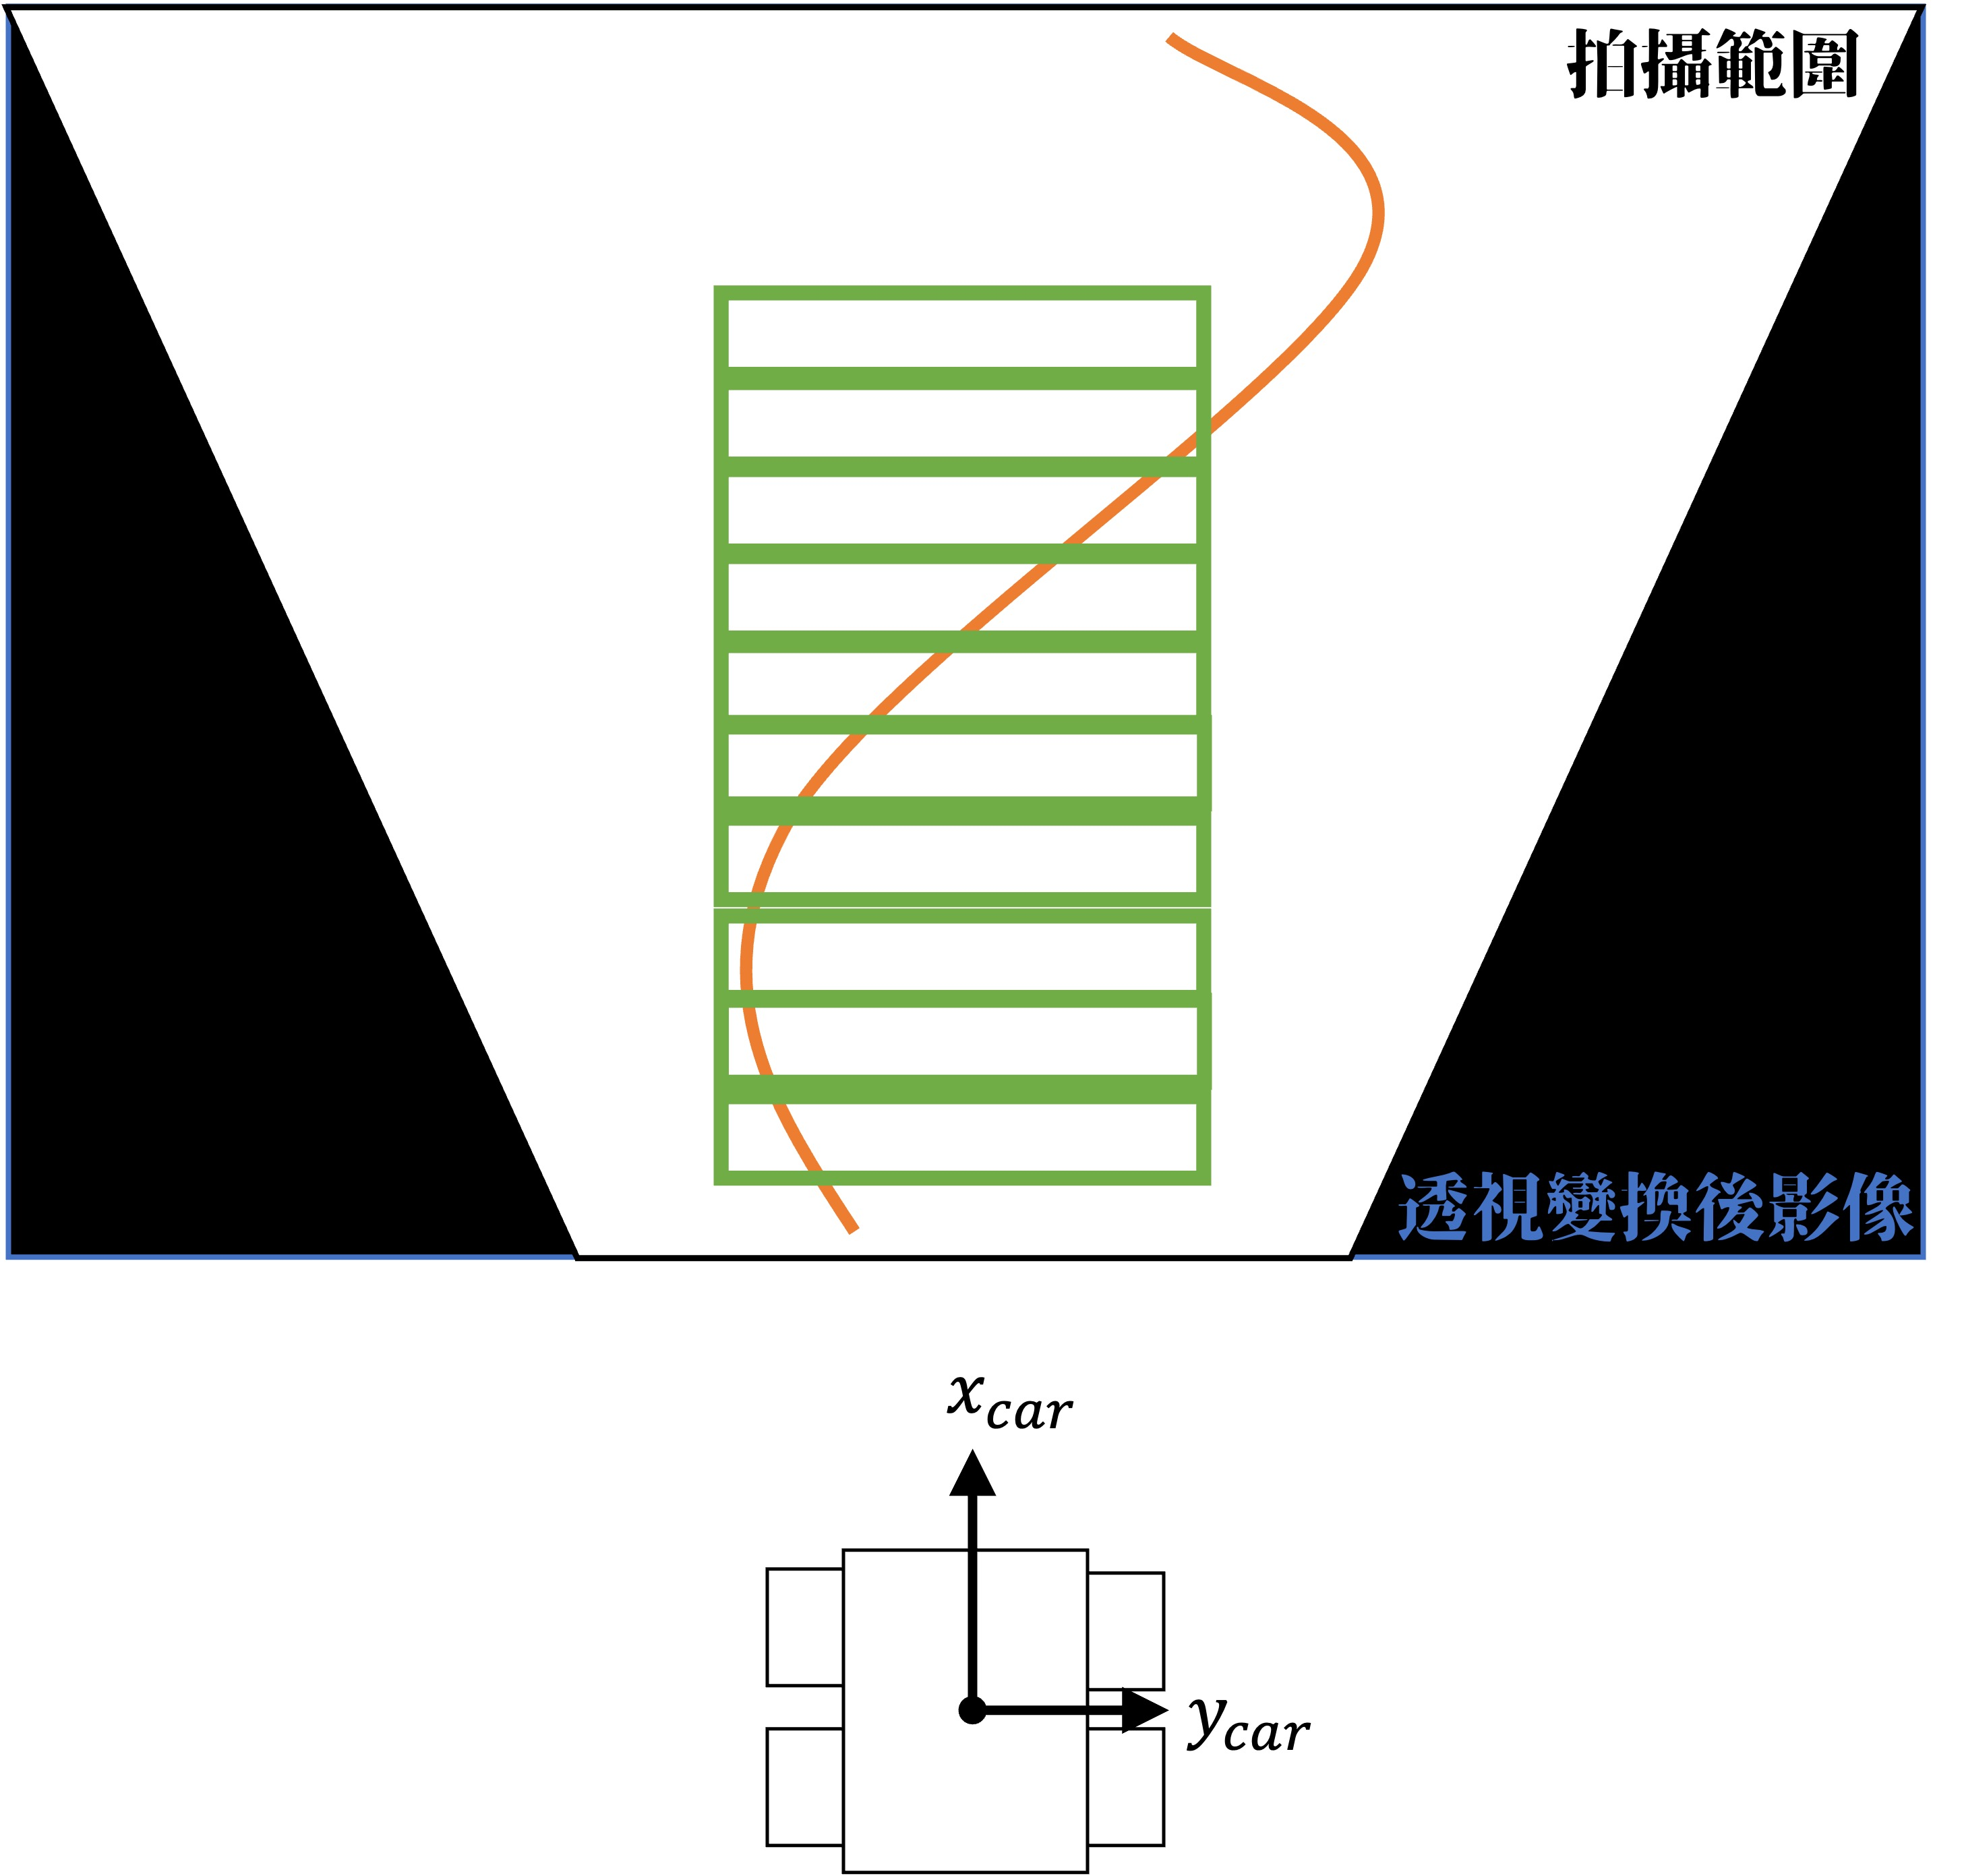
\includegraphics[width=0.7\textwidth]{16.jpg}     %圖片檔案名稱
    \caption{尚未滑動之偵測視窗}    %圖片檔案名稱
    \label{fig:16}    %為圖片添加標籤
    %如\ref{fig:example1}所示
\end{figure}

\begin{figure}[H]
    \centering
    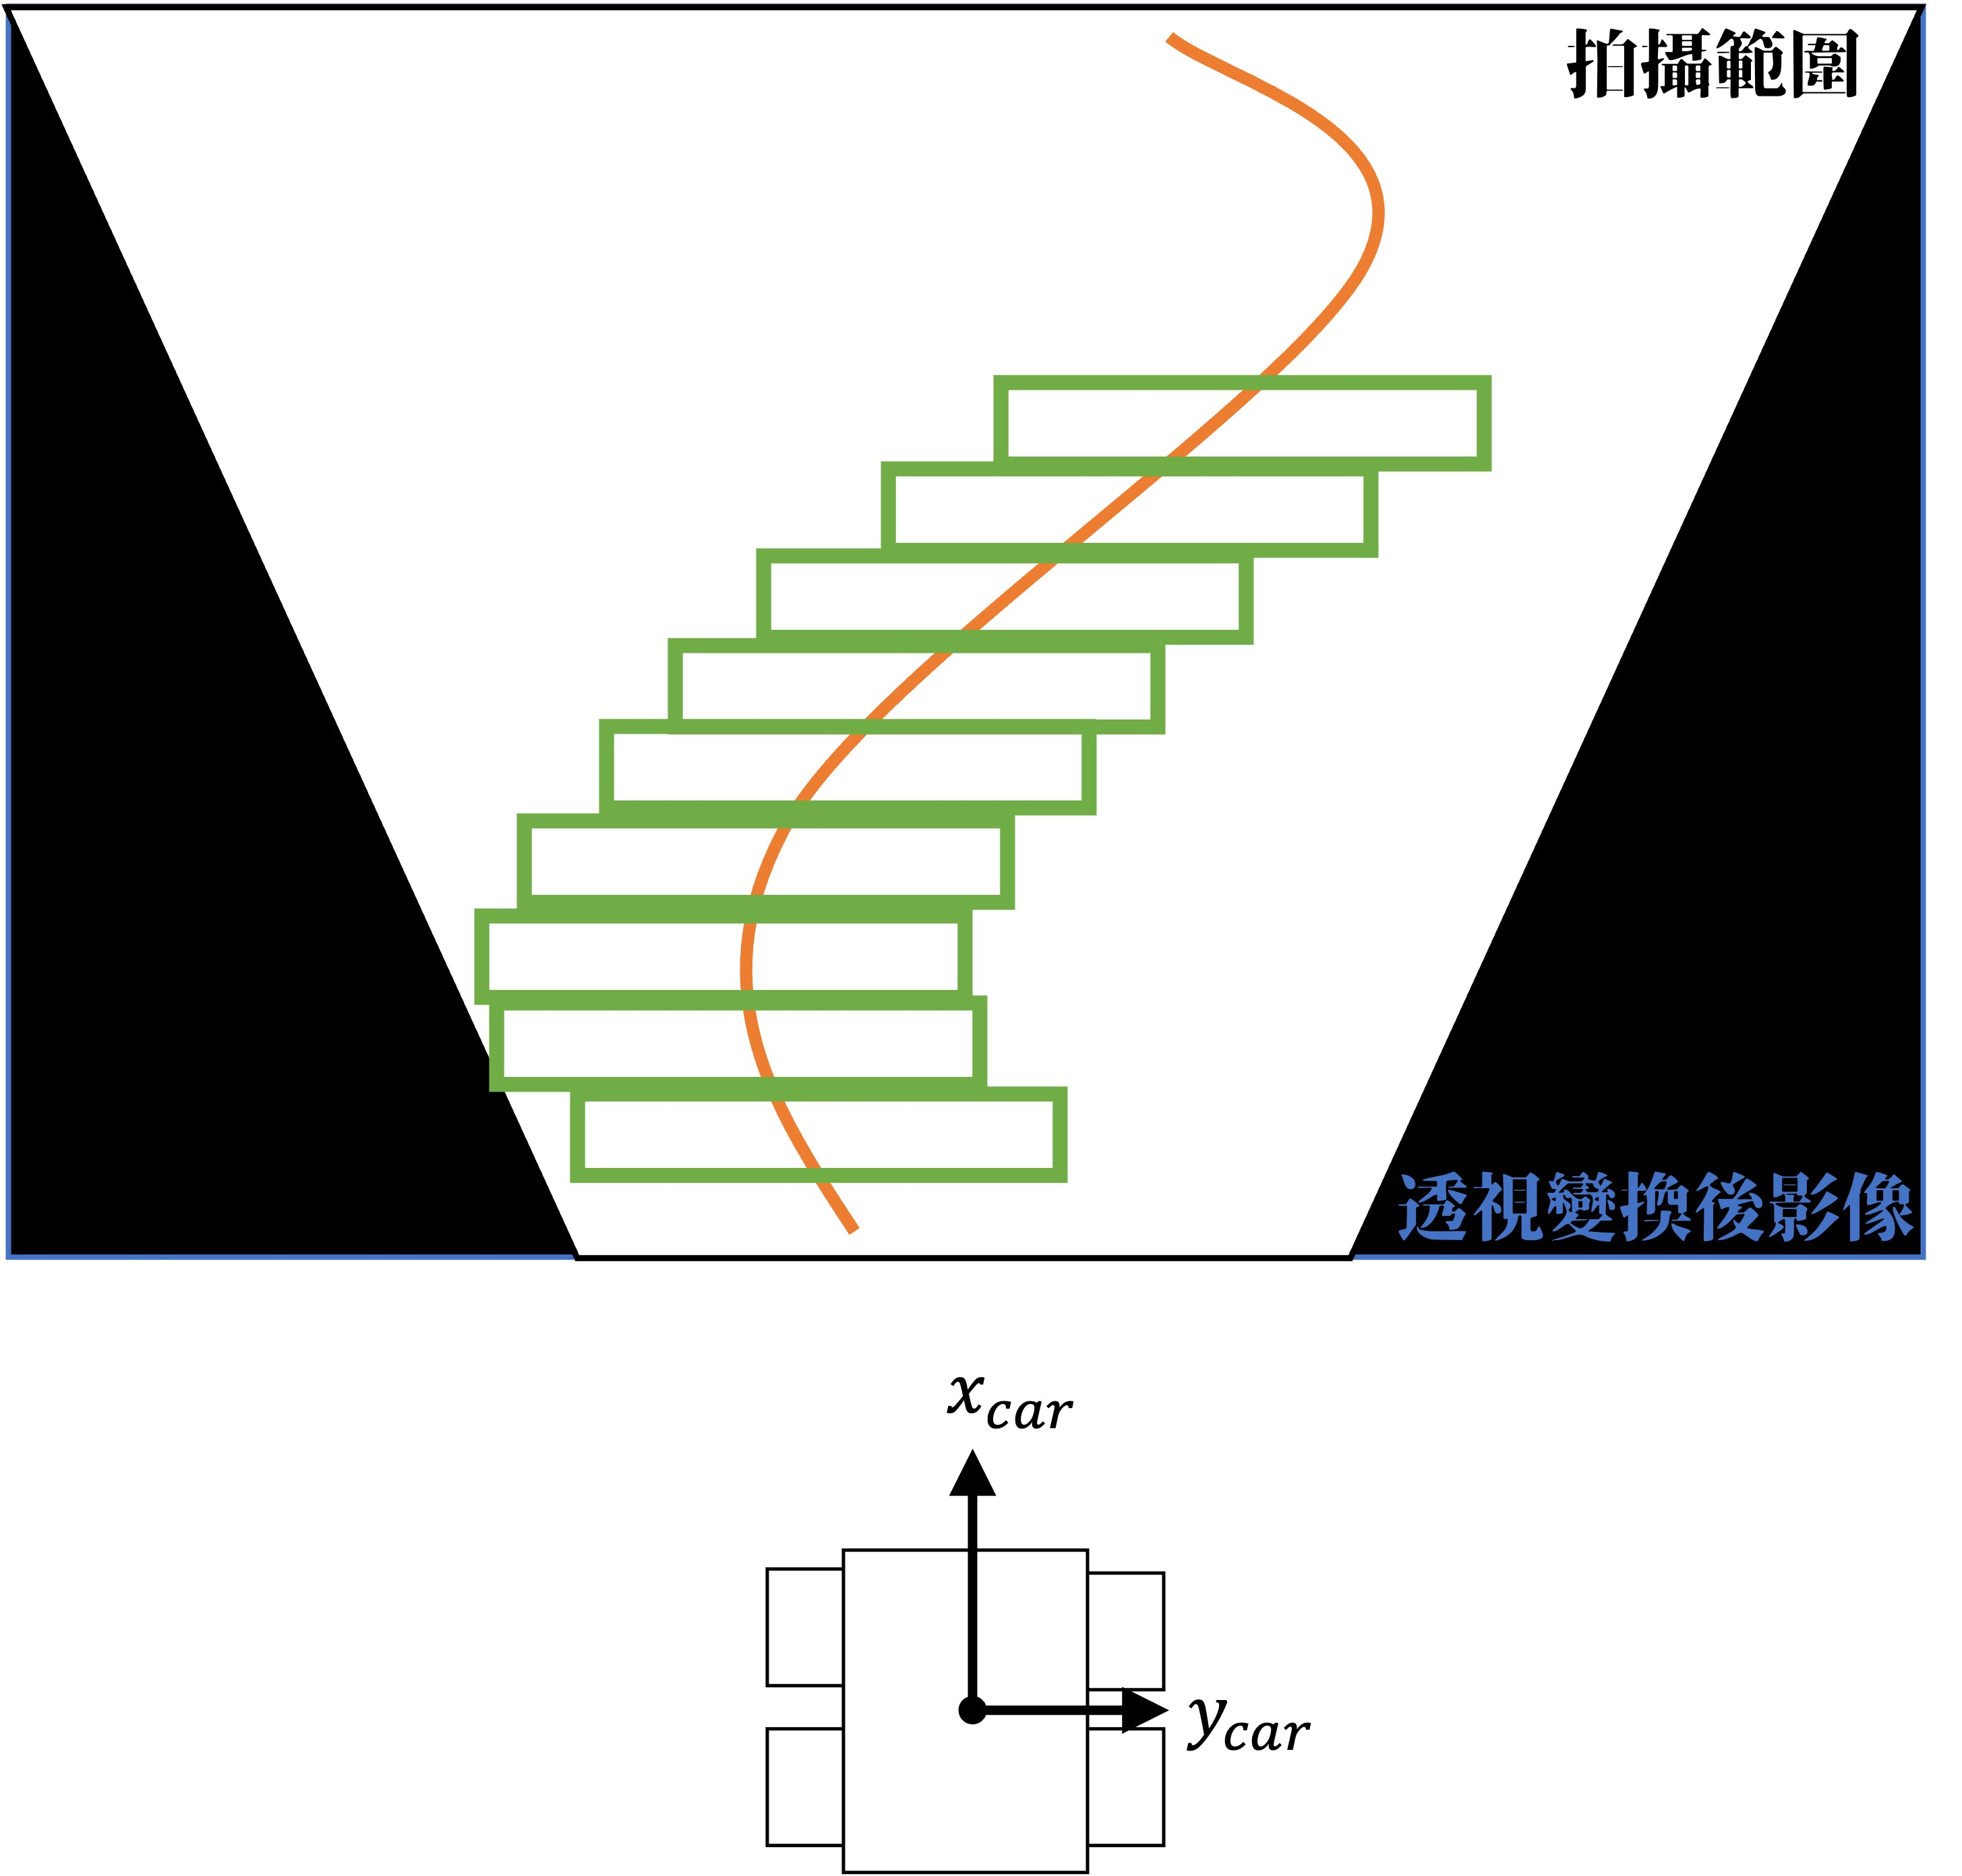
\includegraphics[width=0.7\textwidth]{17.jpg}     %圖片檔案名稱
    \caption{滑動後之偵測視窗}    %圖片檔案名稱
    \label{fig:17}    %為圖片添加標籤
    %如\ref{fig:example1}所示
\end{figure}

據掃描到的像素資料,使用多項式擬合來擬合出車道線或相關物體的曲線,這樣可以準確地描述其形狀。
當獲取到標線像素點後,下一步是利用數學模型來擬合標線的形狀。由於車道標線通常具有一定的連續性與平滑度,可以使用 多項式擬合(Polynomial Fitting) 來描述其形狀。

\hspace{2em}對於普通道路,車道標線通常可以近似為二次曲線: \begin{align} y = ax^2 + bx + c \end{align} 其中,
$a,b,c$ 為待求的係數。使用最小二乘法(Least Squares Method, LSM) 來找到最適合這些數據點的曲線。
\begin{figure}[H]
    \centering
    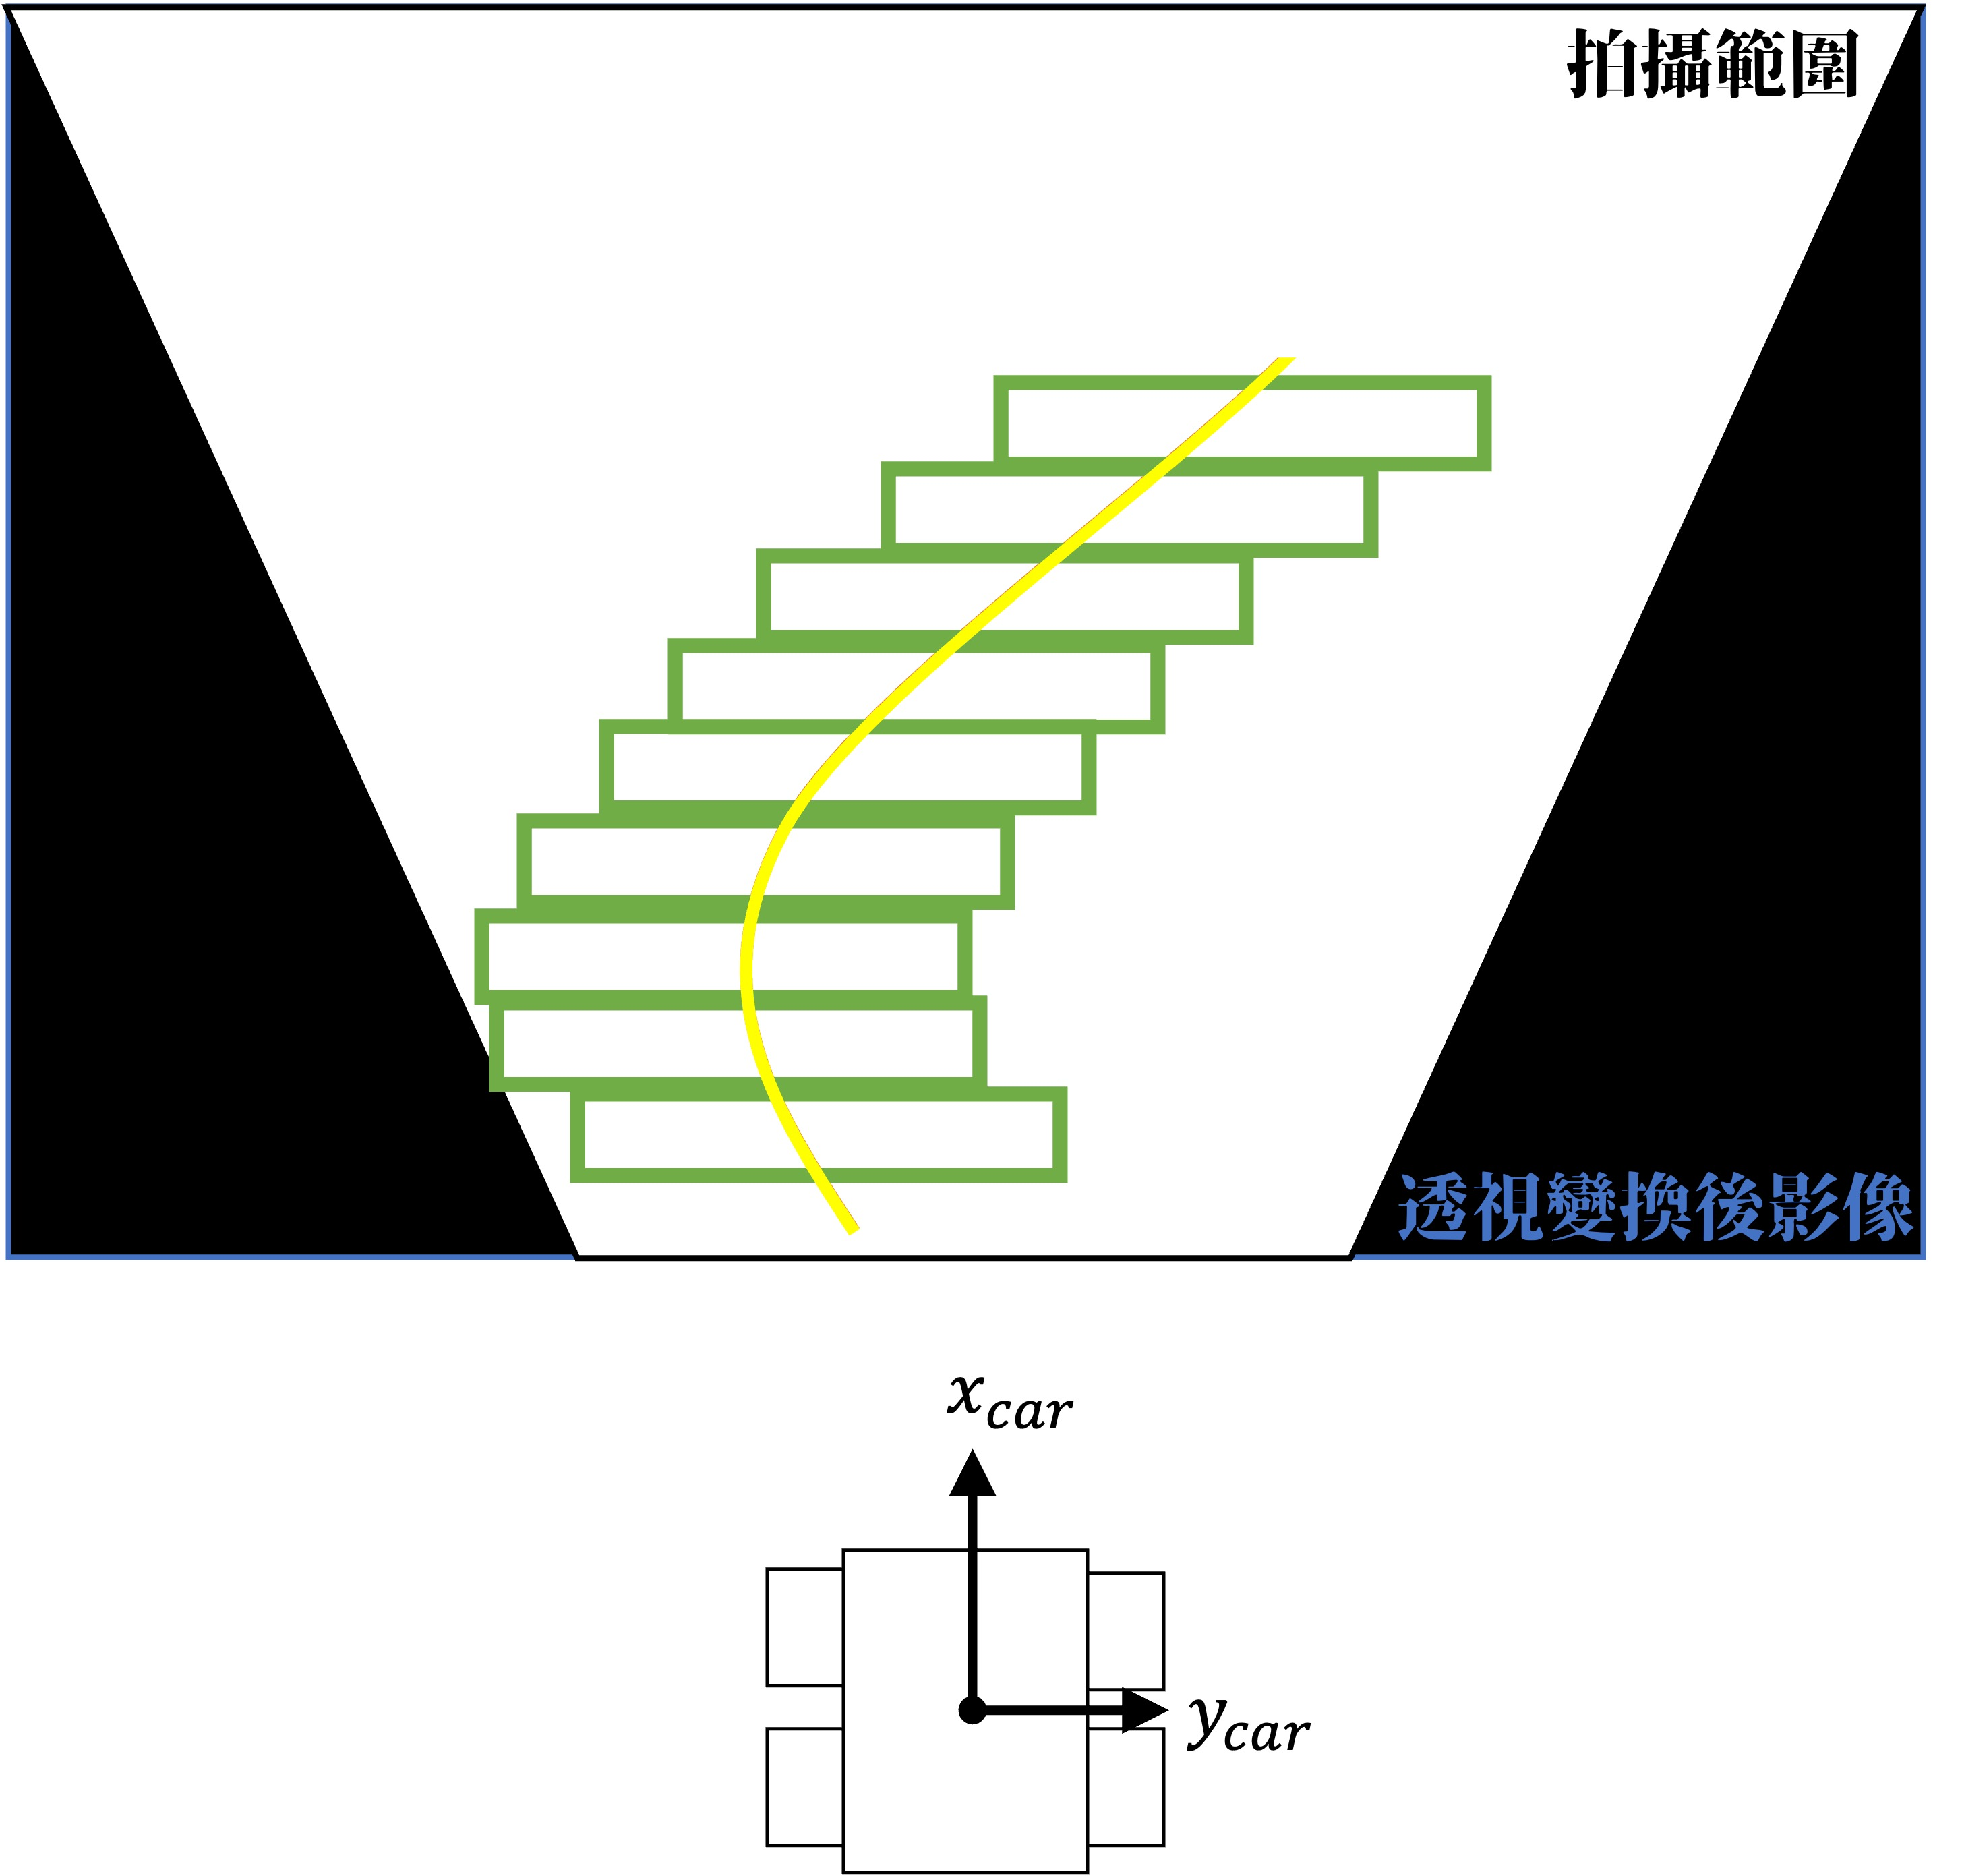
\includegraphics[width=0.7\textwidth]{18.jpg}     %圖片檔案名稱
    \caption{擬合後曲線}    %圖片檔案名稱
    \label{fig:18}    %為圖片添加標籤
    %如\ref{fig:example1}所示
\end{figure}

最後即可根據擬合的曲線與車輛座標系之$x$軸計算車輛的偏移量與偏移角度。

\begin{figure}[H]
    \centering
    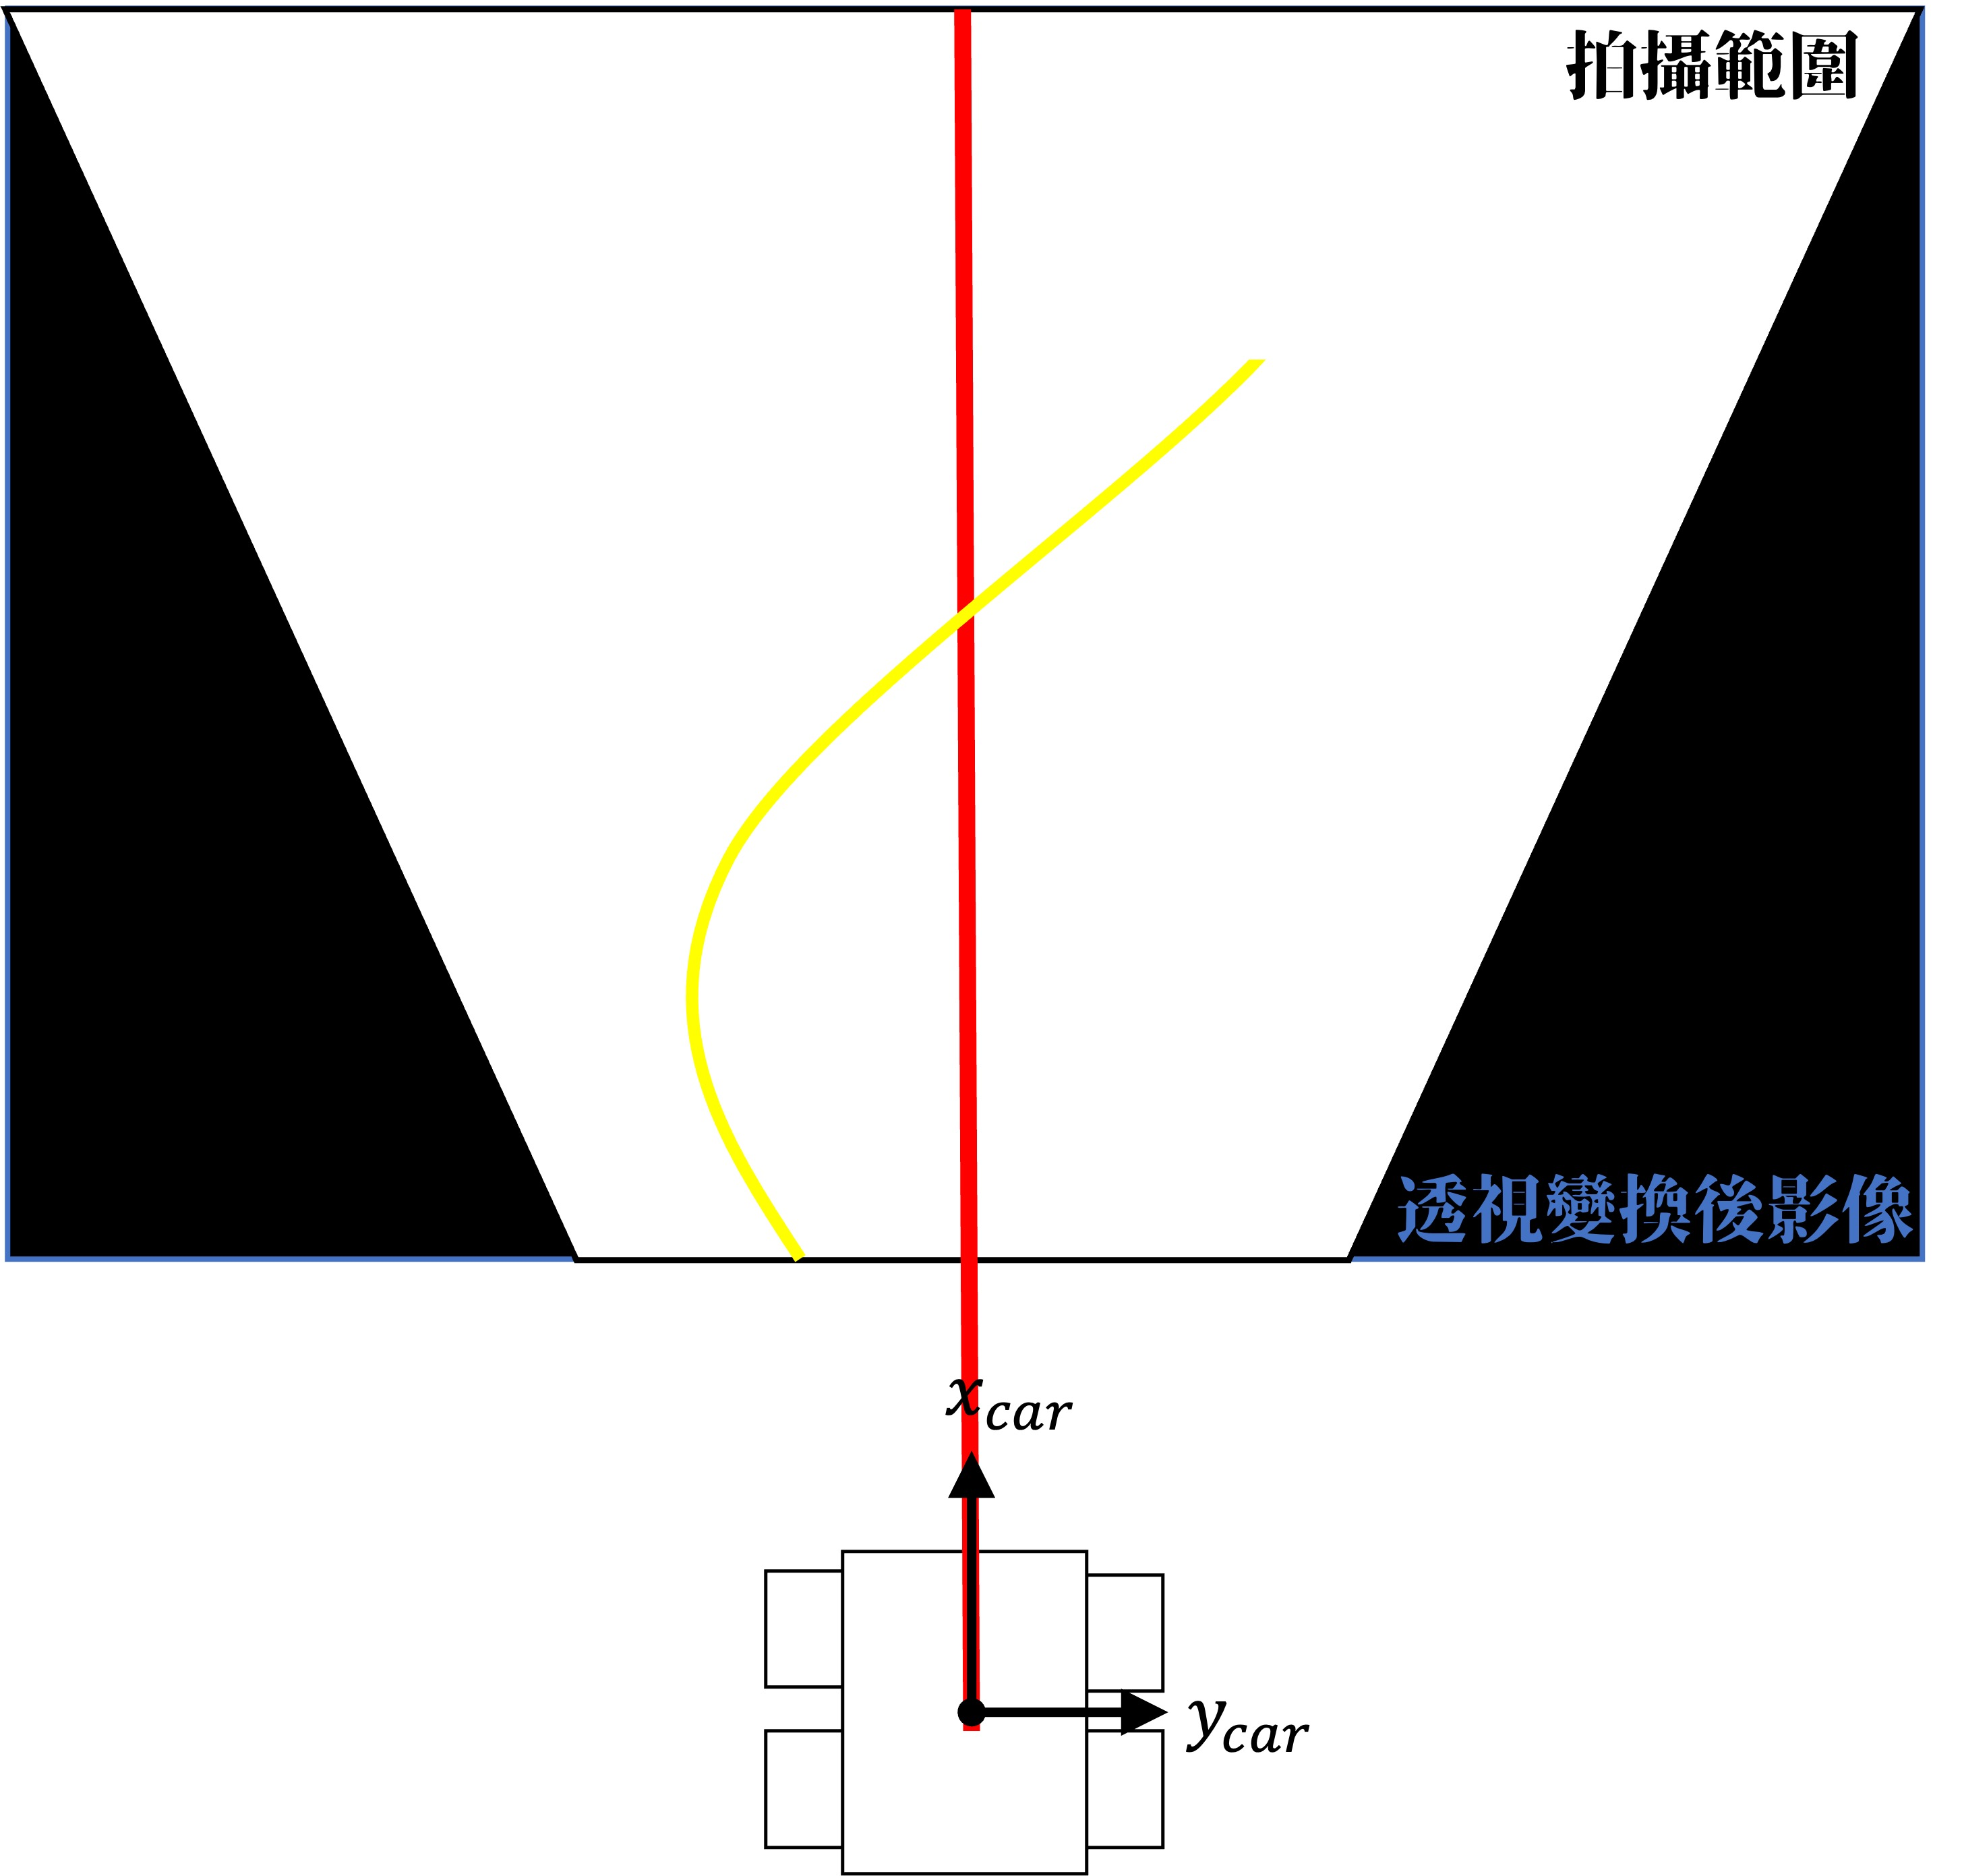
\includegraphics[width=0.7\textwidth]{19.jpg}     %圖片檔案名稱
    \caption{擬合後曲線與車輛座標系之$x$軸}    %圖片檔案名稱
    \label{fig:19}    %為圖片添加標籤
    %如\ref{fig:example1}所示
\end{figure}
根據擬合的曲線,計算出車輛當前的偏移量(與目標軌跡的水平距離)和偏移角度(與車道或目標方向的夾角)。這些數據將作為車輛調整行駛路徑的依據。
%==============================內文==============================

\subsubsection{模糊控制}
%==============================內文==============================
首先定義輸入變數與輸出變數。輸入變數為偏差角度$angle(\theta)$及位置偏移量$distance(mm)$。輸入變數為前進速度$V_{x}$、側向數度$V_{y}$與角速度$\omega$ 。

首先定義偏差角度$angle(\theta)$及位置偏移量$distance(mm)$的隸屬函數。

在本系統中,輸入變數包含偏差角度 $angle(\theta)$ 與位置偏移量 $distance$(mm),需先將其模糊化處理。其定義如下:

\begin{align}
    \theta &\in [-30^\circ, 30^\circ], \quad \theta \in \text{angle} = \{ \text{BL}, \text{SL}, \text{Z}, \text{SR}, \text{BR} \} \\
    d &\in [-50\,\text{mm}, 50\,\text{mm}], \quad distance \in \text{position} = \{ \text{BL}, \text{SL}, \text{Z}, \text{SR}, \text{BR} \}
\end{align}

上述模糊集合分別表示:
\begin{itemize}
    \item BL:大左 (Big Left)
    \item SL:小左 (Small Left)
    \item Z:居中 (Zero)
    \item SR:小右 (Small Right)
    \item BR:大右 (Big Right)
\end{itemize}

每個模糊集合都有對應的隸屬函數 $\mu_A(x)$,其映射如下:

\begin{equation}
    \mu_A(x) : X \rightarrow [0, 1]
\end{equation}


偏差角度$angle(\theta)$的隸屬函數如下:
\begin{align}
    \text{angle}_{\text{BL}}(x) = 
    \begin{cases}
    1 & x \le -30 \\
    \frac{x + 30}{15} & -30 < x \le -15 \\
    0 & \text{otherwise}
    \end{cases}    
\end{align}

\begin{align}
    \text{angle}_{\text{SL}}(x) = 
    \begin{cases}
    \frac{x + 30}{15} & -30 < x \le -15 \\
    \frac{-x}{15} & -15 < x \le 0 \\
    0 & \text{otherwise}
    \end{cases}    
\end{align}

\begin{align}
    \text{angle}_{Z}(x) = 
    \begin{cases}
    \frac{x + 15}{15} & -15 < x \le 0 \\
    \frac{15 - x}{15} & 0 < x \le 15 \\
    0 & \text{otherwise}
    \end{cases}    
\end{align}

\begin{align}
    \text{angle}_{\text{SR}}(x) = 
    \begin{cases}
    \frac{x}{15} & 0 < x \le 15 \\
    \frac{30 - x}{15} & 15 < x \le 30 \\
    0 & \text{otherwise}
    \end{cases}    
\end{align}

\begin{align}
    \text{angle}_{\text{BR}}(x) = 
    \begin{cases}
    \frac{x - 15}{15} & 15 < x \le 30 \\
    1 & x \ge 30 \\
    0 & \text{otherwise}
    \end{cases}    
\end{align}

\begin{figure}[H]
    \centering
    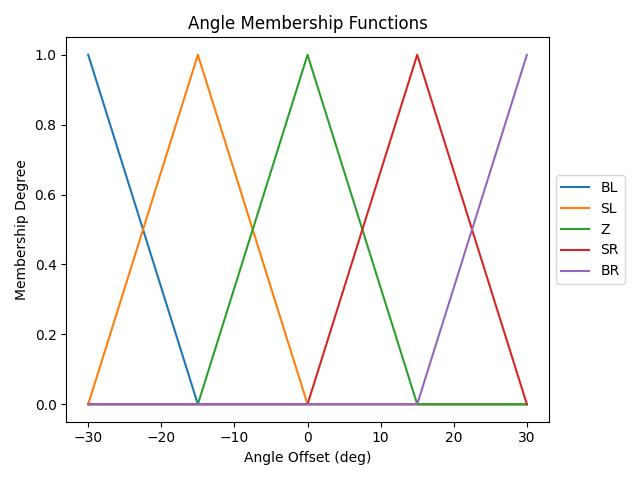
\includegraphics[width=0.7\textwidth]{20.jpg}     %圖片檔案名稱
    \caption{偏差角度$angle(\theta)$隸屬函數}    %圖片檔案名稱
    \label{fig:20}    %為圖片添加標籤
    %如\ref{fig:example1}所示
\end{figure}

位置偏移量$distance(mm)$的隸屬函數如下:

\begin{align}
    \text{distance}_{\text{BL}}(x) = 
    \begin{cases}
    1 & x \le -50 \\
    \frac{x + 50}{25} & -50 < x \le -25 \\
    0 & \text{otherwise}
    \end{cases}    
\end{align}

\begin{align}
    \text{distance}_{\text{SL}}(x) = 
    \begin{cases}
    \frac{x + 50}{25} & -50 < x \le -25 \\
    \frac{-x}{25} & -25 < x \le 0 \\
    0 & \text{otherwise}
    \end{cases}    
\end{align}

\begin{align}
    \text{distance}_{Z}(x) = 
    \begin{cases}
    \frac{x + 25}{25} & -25 < x \le 0 \\
    \frac{25 - x}{25} & 0 < x \le 25 \\
    0 & \text{otherwise}
    \end{cases}    
\end{align}

\begin{align}
    \text{distance}_{\text{SR}}(x) = 
    \begin{cases}
    \frac{x}{25} & 0 < x \le 25 \\
    \frac{50 - x}{25} & 25 < x \le 50 \\
    0 & \text{otherwise}
    \end{cases}    
\end{align}

\begin{align}
    \text{distance}_{\text{BR}}(x) = 
    \begin{cases}
    \frac{x - 25}{25} & 25 < x \le 50 \\
    1 & x \ge 50 \\
    0 & \text{otherwise}
    \end{cases}    
\end{align}

\begin{figure}[H]
    \centering
    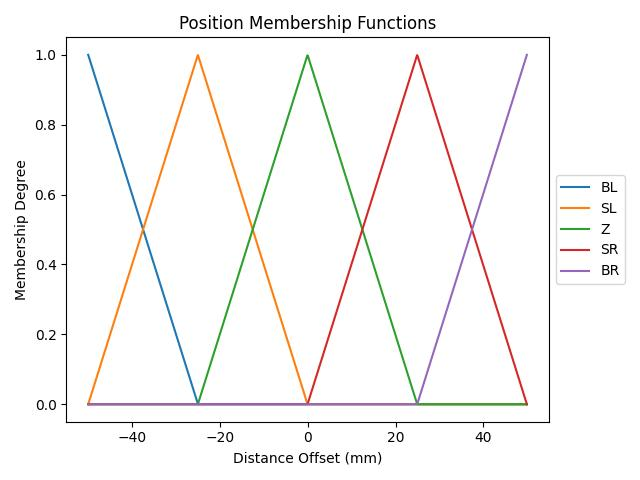
\includegraphics[width=0.7\textwidth]{21.jpg}     %圖片檔案名稱
    \caption{位置偏移量$distance(mm)$隸屬函數}    %圖片檔案名稱
    \label{fig:21}    %為圖片添加標籤
    %如\ref{fig:example1}所示
\end{figure}

接著定義前進速度$V_{x}$、側向數度$V_{y}$與角速度$\omega$的隸屬函數。

前進速度$V_{x}$定義為:
\begin{itemize}
    \item S (Slow):慢速
    \item M (Medium):中速
    \item F (Fast):快速
\end{itemize}

前進速度$V_{x}$的隸屬函數如下:
\begin{align}
    \text{Vx}_{S}(x) = 
    \begin{cases}
    1 & 0 \le x \le 50 \\
    \frac{100 - x}{50} & 50 < x \le 100 \\
    0 & \text{otherwise}
    \end{cases}
\end{align}

\begin{align}
    \text{Vx}_{M}(x) = 
    \begin{cases}
    \frac{x - 50}{50} & 50 < x \le 100 \\
    \frac{150 - x}{50} & 100 < x \le 150 \\
    0 & \text{otherwise}
    \end{cases}
\end{align}

\begin{align}
    \text{Vx}_{F}(x) = 
    \begin{cases}
    \frac{x - 100}{50} & 100 < x \le 150 \\
    1 & 150 < x \le 200 \\
    0 & \text{otherwise}
    \end{cases}    
\end{align}

\begin{figure}[H]
    \centering
    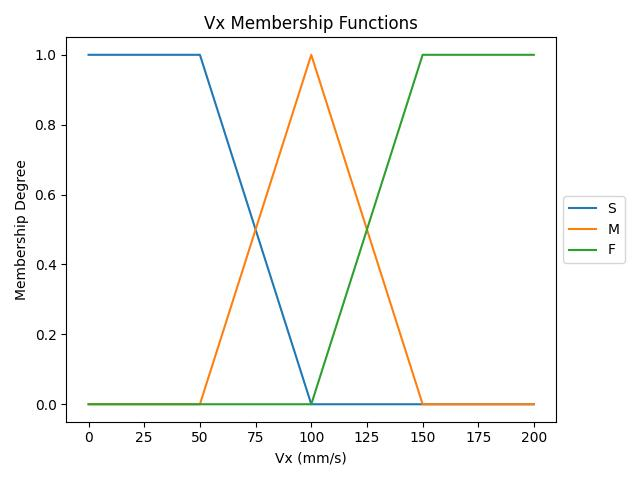
\includegraphics[width=0.8\textwidth]{22.jpg}     %圖片檔案名稱
    \caption{前進速度$V_{x}$隸屬函數}    %圖片檔案名稱
    \label{fig:22}    %為圖片添加標籤
    %如\ref{fig:example1}所示
\end{figure}

側向數度$V_{y}$定義為:
\begin{itemize}
    \item LL (Leftmost):最左
    \item L (Left):左
    \item Z (Zero):中間
    \item R (Right):右
    \item RR (Rightmost):最右
\end{itemize}

側向數度$V_{y}$的隸屬函數如下:

\begin{align}
    \text{Vy}_{LL}(x) = 
    \begin{cases}
    1 & -50 \le x \le -40 \\
    \frac{-20 - x}{20} & -40 < x \le -20 \\
    0 & \text{otherwise}
    \end{cases}       
\end{align}

\begin{align}
    \text{Vy}_{L}(x) = 
    \begin{cases}
    \frac{x + 30}{15} & -30 < x \le -15 \\
    \frac{-x}{15} & -15 < x \le 0 \\
    0 & \text{otherwise}
    \end{cases}    
\end{align}

\begin{align}
    \text{Vy}_{Z}(x) = 
    \begin{cases}
    \frac{x + 15}{15} & -15 < x \le 0 \\
    \frac{15 - x}{15} & 0 < x \le 15 \\
    0 & \text{otherwise}
    \end{cases}     
\end{align}

\begin{align}
    \text{Vy}_{R}(x) = 
    \begin{cases}
    \frac{x}{15} & 0 < x \le 15 \\
    \frac{30 - x}{15} & 15 < x \le 30 \\
    0 & \text{otherwise}
    \end{cases}     
\end{align}

\begin{align}
    \text{Vy}_{RR}(x) = 
    \begin{cases}
    \frac{x - 20}{20} & 20 < x \le 40 \\
    1 & 40 < x \le 50 \\
    0 & \text{otherwise}
    \end{cases}       
\end{align}

\begin{figure}[H]
    \centering
    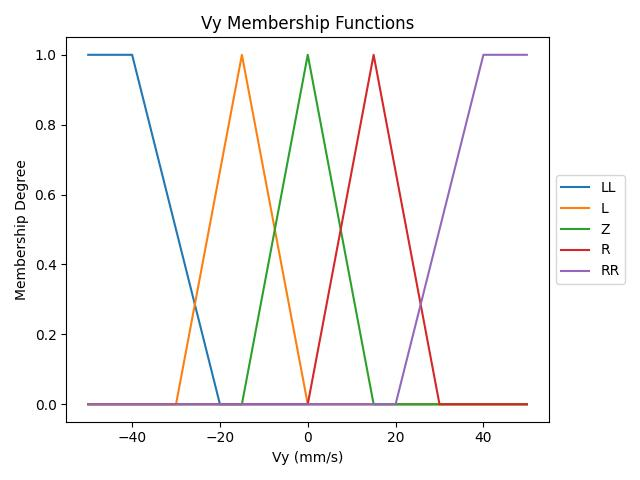
\includegraphics[width=0.8\textwidth]{23.jpg}     %圖片檔案名稱
    \caption{側向數度$V_{y}$隸屬函數}    %圖片檔案名稱
    \label{fig:23}    %為圖片添加標籤
    %如\ref{fig:example1}所示
\end{figure}

角速度$\omega$定義為:
\begin{itemize}
    \item CCW2 (Counterclockwise 2):強烈逆時針
    \item CCW (Counterclockwise):輕微逆時針
    \item Z (Zero):無旋轉
    \item CW (Clockwise):輕微順時針
    \item CW2 (Clockwise 2):強烈順時針
\end{itemize}
角速度$\omega$的隸屬函數如下:

\begin{align}
    \omega_{\text{CCW2}}(x) = 
    \begin{cases}
    1 & -20 \le x \le -15 \\
    \frac{-10 - x}{5} & -15 < x \le -10 \\
    0 & \text{otherwise}
    \end{cases}    
\end{align}

\begin{align}
    \omega_{\text{CCW}}(x) = 
    \begin{cases}
    \frac{x + 15}{5} & -15 < x \le -10 \\
    \frac{-x}{10} & -10 < x \le 0 \\
    0 & \text{otherwise}
    \end{cases}     
\end{align}

\begin{align}
    \omega_{Z}(x) = 
    \begin{cases}
    \frac{x + 10}{10} & -10 < x \le 0 \\
    \frac{10 - x}{10} & 0 < x \le 10 \\
    0 & \text{otherwise}
    \end{cases}    
\end{align}

\begin{align}
    \omega_{\text{CW}}(x) = 
    \begin{cases}
    \frac{x}{10} & 0 < x \le 10 \\
    \frac{15 - x}{5} & 10 < x \le 15 \\
    0 & \text{otherwise}
    \end{cases}      
\end{align}

\begin{align}
    \omega_{\text{CW2}}(x) = 
    \begin{cases}
    \frac{x - 10}{5} & 10 < x \le 15 \\
    1 & 15 < x \le 20 \\
    0 & \text{otherwise}
    \end{cases}      
\end{align}

\begin{figure}[H]
    \centering
    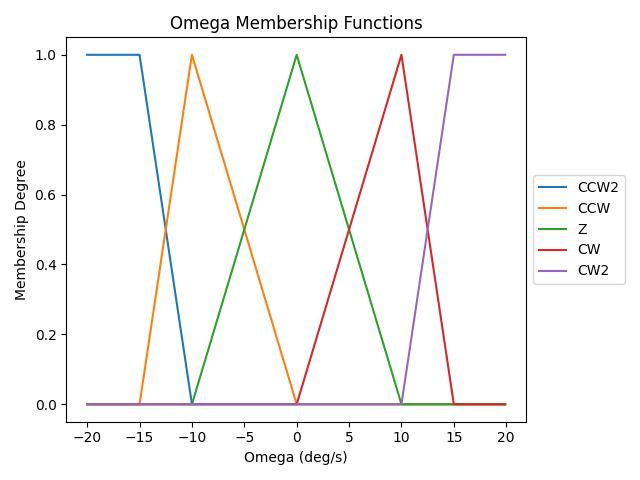
\includegraphics[width=0.8\textwidth]{24.jpg}     %圖片檔案名稱
    \caption{角速度$\omega$隸屬函數}    %圖片檔案名稱
    \label{fig:24}    %為圖片添加標籤
    %如\ref{fig:example1}所示
\end{figure}

接著是定義控制規則庫,$V_{x}$之控制規則表、$V_{y}$控制規則表與$\omega$控制規則表,如下所示。

\begin{table}[H]
    \centering
    \caption{$V_{x}$控制規則表}
    \vspace{6pt} % 增加空格
    \begin{tabular}{|c|c|c|c|c|c|}
    \hline
    \diagbox{\textbf{Angle($^\circ$)}}{\textbf{Position(cm)}} & \textbf{BL} & \textbf{SL} & \textbf{Z} & \textbf{SR} & \textbf{BR} \\
    \hline
    \textbf{BL} & S & S & M & S & S \\
    \hline
    \textbf{SL} & S & M & F & M & S \\
    \hline
    \textbf{Z} & M & F & F & F & M \\
    \hline
    \textbf{SR} & S & M & F & M & S \\
    \hline
    \textbf{BR} & S & S & M & S & S \\
    \hline
    \end{tabular}
    \label{tab:fu1}
\end{table}

\begin{table}[H]
    \centering
    \caption{$V_{y}$控制規則表}
    \vspace{6pt} % 增加空格
    \begin{tabular}{|c|c|c|c|c|c|}
    \hline
    \diagbox{\textbf{Angle($^\circ$)}}{\textbf{Position(cm)}}& \textbf{BL} & \textbf{SL} & \textbf{Z} & \textbf{SR} & \textbf{BR} \\
    \hline
    \textbf{BL} & RR & R & Z & L & LL \\
    \hline
    \textbf{SL} & RR & R & Z & L & LL \\
    \hline
    \textbf{Z} & RR & R & Z & L & LL \\
    \hline
    \textbf{SR} & RR & R & Z & L & LL \\
    \hline
    \textbf{BR} & RR & R & Z & L & LL \\
    \hline
    \end{tabular}
    \label{tab:fu2}
\end{table}

\begin{table}[H]
    \centering
    \caption{$\omega$控制規則表}
    \vspace{6pt} % 增加空格
    \begin{tabular}{|c|c|c|c|c|c|}
    \hline
    \diagbox{\textbf{Angle($^\circ$)}}{\textbf{Position(cm)}}& \textbf{BL} & \textbf{SL} & \textbf{Z} & \textbf{SR} & \textbf{BR} \\
    \hline
    \textbf{BL} & CW2 & CW2 & CW2 & CW2 & CW2 \\
    \hline
    \textbf{SL} & CW & CW & CW & CW & CW \\
    \hline
    \textbf{Z} & Z & Z & Z & Z & Z \\
    \hline
    \textbf{SR} & CCW & CCW & CCW & CCW & CCW2 \\
    \hline
    \textbf{BR} & CCW2 & CCW2 & CCW2 & CCW2 & CCW2 \\
    \hline
    \end{tabular}
    \label{tab:fu3}
\end{table}
觸發強度是由這兩個模糊集合的隸屬度中的較小者所決定。
\begin{align}
        \alpha_{ij} = \min\left( \mu^{A_i}_{\text{angle}}(\theta),\ \mu^{B_j}_{\text{position}}(x) \right)
\end{align}

最後進行去模糊化,計算對每個輸出變數$z$,計算:

\begin{align}
    z^* = \frac{\int z \cdot \mu(z) \, dz}{\int \mu(z) \, dz}    
\end{align}

其中,$\mu(z)$是合併後的輸出模糊集合的隸屬度。

因為有數組輸出,利用Alpha-Cut($\alpha$-截集)的方式,排除異常值,僅保留後 80\% 結果來避免極端值干擾。

對輸出值集合${z_i}$,排序後選取前$N \times \alpha$個,再取平均:
\begin{align}
    \bar{z}_\alpha = \frac{1}{N_\alpha} \sum_{i=1}^{N_\alpha} z_i 
\end{align}

最後即可取得不同偏差角度$angle$及位置偏移量$distance$對應之前進速度$V_{x}$(圖\ref{fig:25})、側向數度$V_{y}$(圖\ref{fig:26})與角速度$\omega$(圖\ref{fig:27})。

\begin{figure}[H]
    \centering
    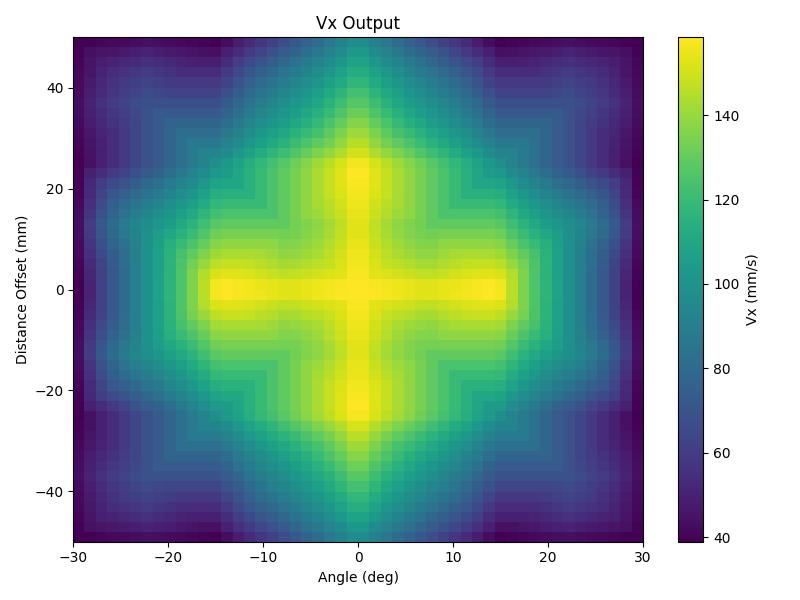
\includegraphics[width=0.8\textwidth]{25.jpg}     %圖片檔案名稱
    \caption{不同偏差角度及偏移量對應之前進速度$V_{x}$}    %圖片檔案名稱
    \label{fig:25}    %為圖片添加標籤
    %如\ref{fig:example1}所示
\end{figure}

\begin{figure}[H]
    \centering
    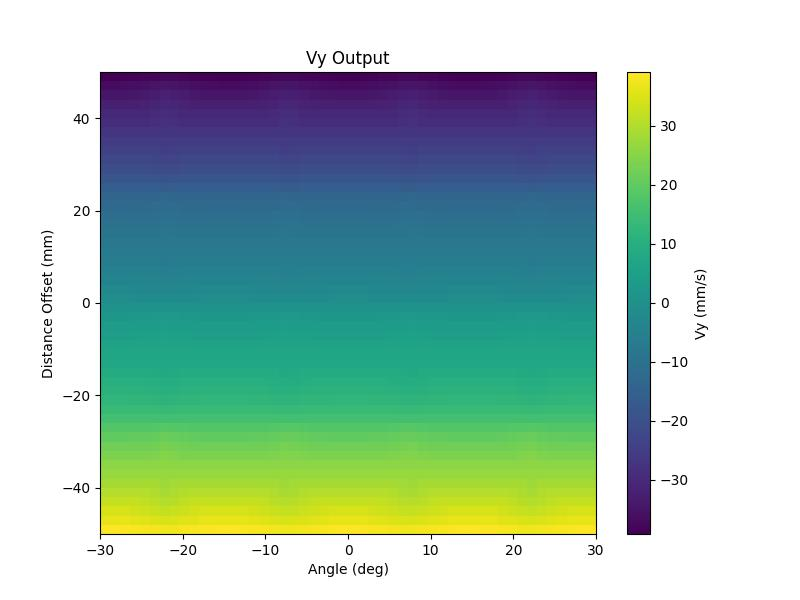
\includegraphics[width=0.8\textwidth]{26.jpg}     %圖片檔案名稱
    \caption{不同偏差角度及偏移量對應之側向數度$V_{y}$}    %圖片檔案名稱
    \label{fig:26}    %為圖片添加標籤
    %如\ref{fig:example1}所示
\end{figure}

\begin{figure}[H]
    \centering
    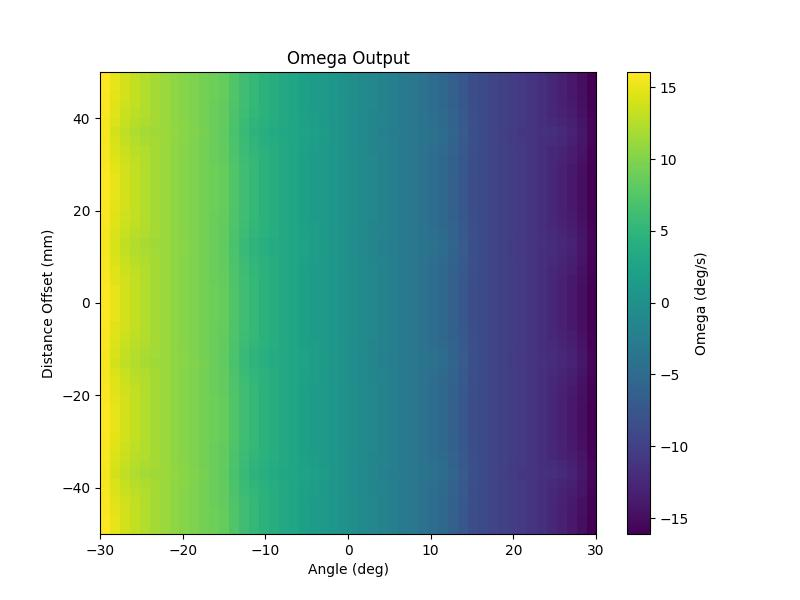
\includegraphics[width=0.8\textwidth]{27.jpg}     %圖片檔案名稱
    \caption{不同偏差角度及偏移量對應之角速度$\omega$}    %圖片檔案名稱
    \label{fig:27}    %為圖片添加標籤
    %如\ref{fig:example1}所示
\end{figure}
%==============================內文==============================

\section{\centering 模擬與分析}
%==============================內文==============================
\hspace{2em}

%==============================內文==============================

\section{\centering 製程與實作}
%==============================內文==============================
\hspace{2em}

%==============================內文==============================

\section{\centering 測試與驗證}
%==============================內文==============================
\hspace{2em}

%==============================內文==============================

\section{\centering 結論與反思}
%==============================內文==============================
\hspace{2em}


%==============================內文==============================




\section{\centering 參考文獻}
%==============================內文==============================
\renewcommand{\refname}{}  % 去除 "References" 標題
\printbibliography  % 列出參考文獻
%==============================內文==============================

\section{\centering 附錄}

\subsection{程式碼} 
%==============================內文==============================
\hspace{2em}
%==============================內文==============================

\subsection{物料清單與發票收據} 
%==============================內文==============================
\hspace{2em}
\begin{figure}[H]
    \centering
    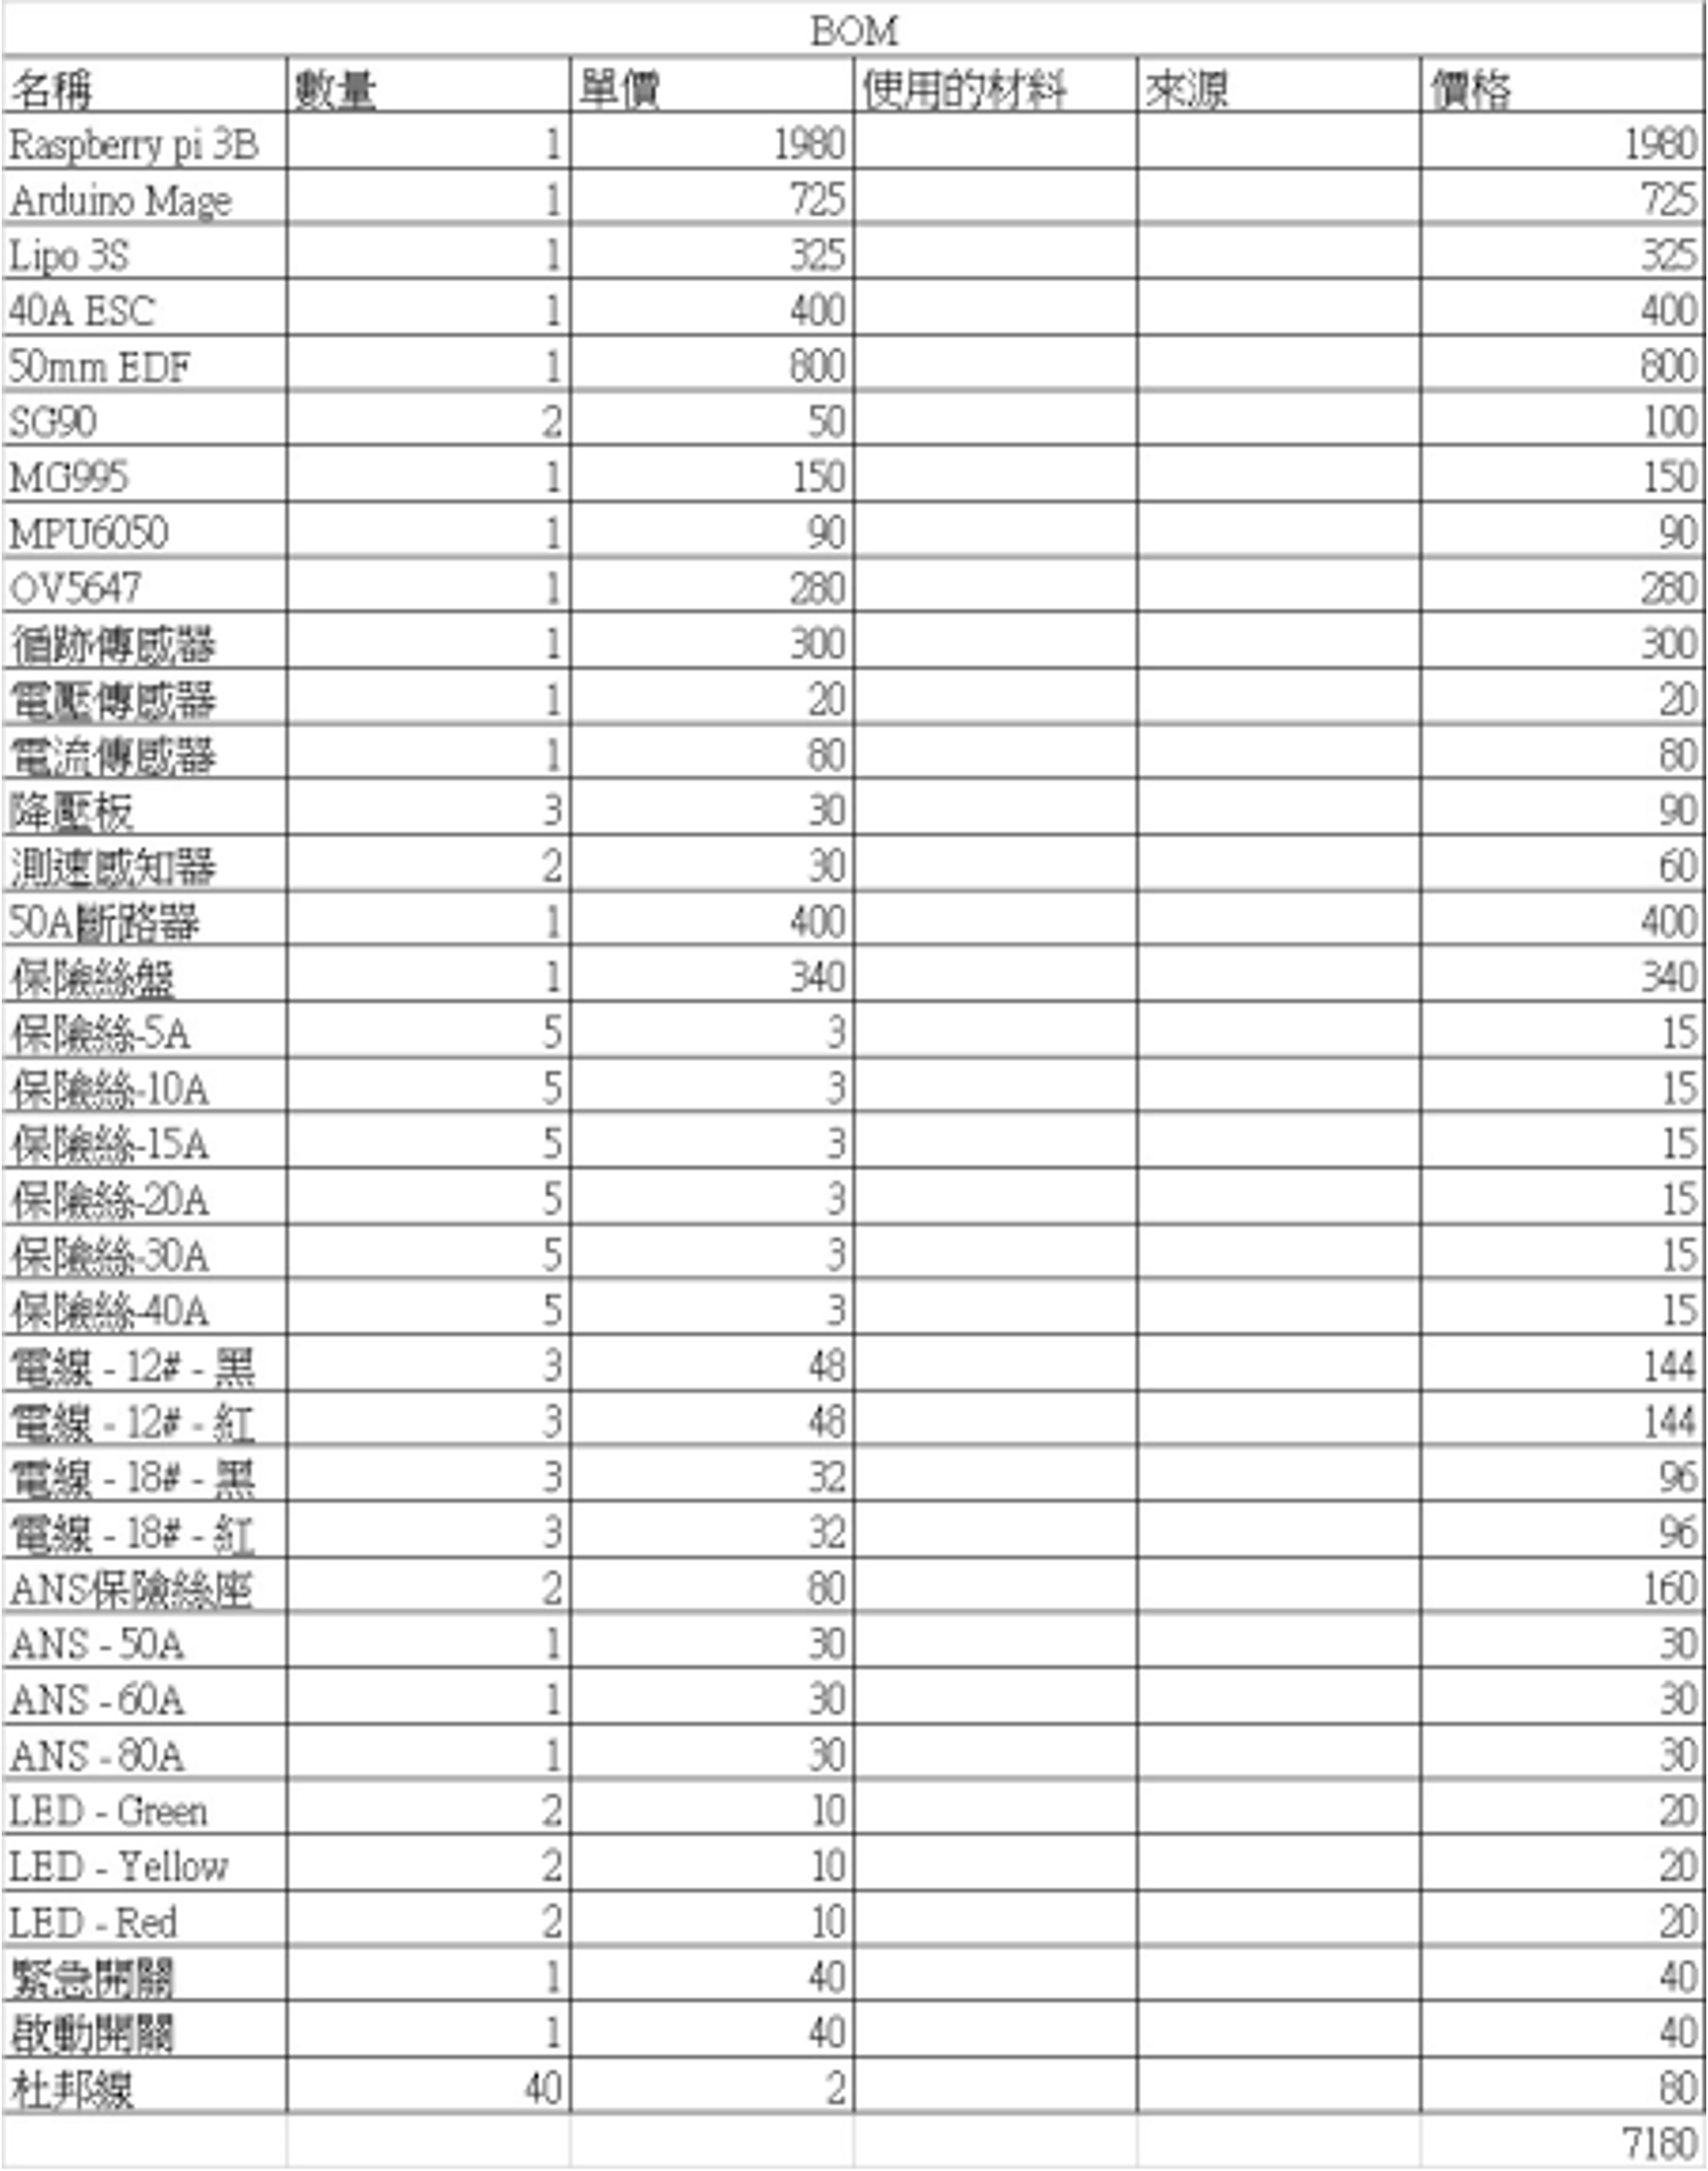
\includegraphics[width=0.8\textwidth]{8.jpg}     %圖片檔案名稱
    \caption{bom表}    %圖片檔案名稱
    \label{fig:8}    %為圖片添加標籤
    %如\ref{fig:example1}所示
\end{figure}
%==============================內文==============================


\end{document}

%=============================================================================================================================
%=============================================================================================================================
%=============================================================================================================================


\begin{comment}

\section{\centering 緒論}
\subsection{研究問題} 
\subsubsection{違規車輛偵測}
    
%==============================圖片==============================

\begin{figure}[H]
    \centering
    \includegraphics[width=0.7\textwidth]{截圖 2025-01-24 03.21.17.jpg}     %圖片檔案名稱
    \caption{這是圖片的標題}    %圖片檔案名稱
    \label{fig:example2}    %為圖片添加標籤
    %如\ref{fig:example1}所示
\end{figure}
    
%==============================數學公式==============================

\begin{align}
    a &= b + c \label{eq:1}
    \\
    d &= e - f \label{eq:2}
    %式\ref{eq:2}
\end{align}
    
%==============================表格==============================

\begin{table}[H]
    \centering
    \caption{致動器的功能與數目列表}
    \vspace{6pt} % 增加空格
    \label{tab:c}
    \begin{tabular}{lll}
        \toprule
        \textbf{項目} & \textbf{功能} & \textbf{數量}\\
        \midrule
        Wemos D1  & 接收個人電腦指令控制l298n &1\\
        ESP32-CAM  & 拍攝影像並傳輸至個人電腦 &1\\
        MacBook M1  & 影像偵測與控制演算法計算 &1\\
        l298n  & 麥克納姆輪 &2\\
        \bottomrule
    \end{tabular}
    %如\ref{tab:TT2}所示
\end{table}
    
\begin{table}[H]
    \centering
    \caption{C922 Pro Stream 規格}
    \vspace{6pt} % 增加空格
    \label{tab:C922 Pro}
    \begin{tabular}{ll}
        \toprule
        \textbf{項目} & \textbf{規格} \\
        \midrule
        解析度  & 1280$\times$720 (HD) \\
        幀率  & 30fps \\
        水平視角 & 70.42$^\circ$ \\
        垂直視角  & 43.3$^\circ$ \\
        \bottomrule
    \end{tabular}
\end{table}

%==============================條列==============================

%無序條列

\begin{itemize}
    \item 第一項
    \item 第二項
    \item 第三項
\end{itemize}

%有序條列

\begin{enumerate}
    \item 第一項
    \item 第二項
    \item 第三項
\end{enumerate}

    \end{comment}
        